%-------------------------------------------------------------------------------
%                            BAB IV
%               		HASIL DAN PEMBAHASAN
%-------------------------------------------------------------------------------
\fancyhf{} 
\fancyfoot[C]{\thepage}
\chapter{HASIL DAN PEMBAHASAN}

\section{\uppercase{Identifikasi Masalah}}
Adapun hasil dari tahapan identifikasi masalah adalah sebagai berikut:

\begin{itemize}
	\item Sistem pemasaran saat ini masih dilakukan secara datang langsung ke tempat penjualan atau memesan lewat aplikasi media sosial.
	\item Pelanggan tidak dapat mengetahui ketersediaan stok produk sebelum bertanya kepada penjual atau mengunjungi langsung tempat penjualannya.
	\item Susahnya menjaga kestabilan harga produk antar penjual tanaman hidroponik.
\end{itemize}

\section{\uppercase{Analisis Kebutuhan}}
Analisa kebutuhan merupakan tahapan untuk mengevaluasi dan menguraikan setiap permasalahan dan informasi terkait sistem yang bertujuan untuk membantu dalam pembuatan aplikasi ke depannya. Pada penelitian ini analisis kebutuhan sistem
terdiri dari menentukan kelompok pengguna dan Use case Diagram. Hasil daripada analisis kebutuhan dapat dilihat di bawah ini:

\subsection{Kelompok Pengguna}
Pengguna yang akan menggunakan aplikasi web ini dapat dikelompokkan menjadi dua kelompok, yaitu:

\begin{enumerate}
	\item Admin
		\par Admin adalah orang yang mengelola aplikasi seperti mendaftarkan penjual baru, membuat promo diaplikasi dan memantau pengguna.
	
	\item Penjual
		 \par Penjual adalah kelompok pengguna yang menggunakan aplikasi bertujuan untuk menjual produknya yaitu tanaman hidroponik kepada calon pembeli.
\end{enumerate}

\subsection{Use Case Diagram}
Use case diagram adalah diagram yang menjelaskan interaksi antara komponen atau pihak yang terkait (aktor) dan sistem. selain itu Use case diagram dapat mendeskripsikan kebutuhan fungsional dari aplikasi sehingga dapat mengetahui apa saja yang dapat dilakukan oleh sistem. setiap case yang terdapat di
dalam Use case akan menjadi fitur aplikasi pada tahap pembuatan aplikasinya. Berikut merupakan gambaran Use case diagram untuk aplikasi penjualan tanaman hidroponik berbasis web :

\begin{figure}[H]
	\centering
	{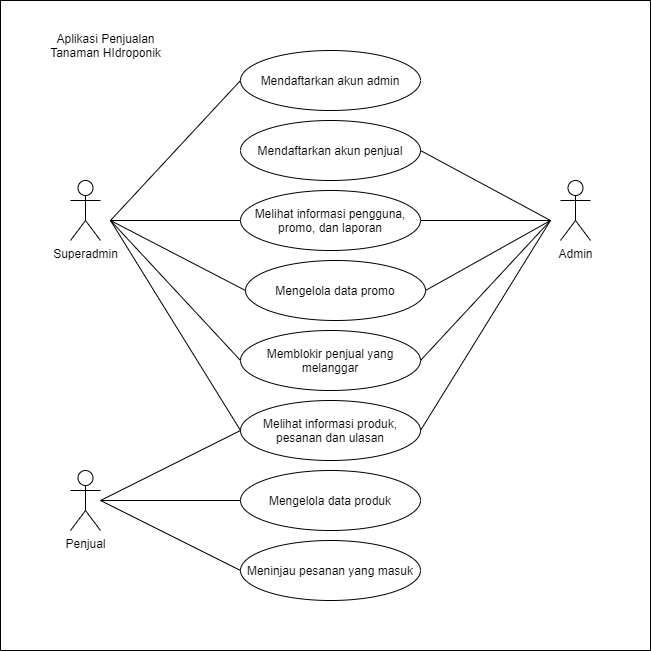
\includegraphics [width = 14cm, height= 14cm]{gambar/use_case_diagram}}
	\caption{Use Case Diagram}
	\label{use_case_diagram}
\end{figure}

\par Gambar 4.1 merupakan Use case yang menjelaskan interaksi antara superadmin, admin dan penjual dengan sistem aplikasi. Dimana level yang paling tinggi di sistem ini adalah superadmin yang bertindak untuk mendaftarkan admin, lalu nantinya para admin inilah yang bertugas mendaftarkan para penjual yang ingin menjual produknya di aplikasi AgriHub ini. Superadmin dan admin disini dapat memantau informasi semua pengguna yang sudah terdaftar diaplikasi baik itu penjual maupun pembeli yang mendaftar lewat aplikasi android dan dapat melihat produk-produk apa saja yang telah diupload oleh para penjual, serta dapat menghapusnya jika dianggap tidak sesuai. Superadmin dan admin juga dapat melihat semua pesanan yang sudah terjadi antara penjual dengan pembeli, melihat ulasan dari pembeli terhadap produk yang dibeli dari penjual serta dapat mengadakan promo sesekali di aplikasinya dan dapat melihat laporan yang masuk dari pembeli terhadap penjual serta dapat mengambil tindakan seperti memblokir penjual tersebut dari sistem.

\par Sedangkan dari sisi aktor penjual. Setelah penjual didaftarkan oleh admin, penjual harus memverifikasi emailnya terlebih dahulu sebelum bisa menggunakan aplikasinya. Baru setelah verifikasi email penjual dapat menggunakan aplikasinya untuk menambahkan produk yang ingin dijualnya, mengelolanya seperti mengubah dan menghapus produk, menerima pesanan dari pembeli dan mengubah statusnya dari belum menjadi diproses, dikirim dan sampai selesai. Penjual juga dapat melihat ulasan-ulasan dari pembeli terhadap pesanan dan produk yang ia jual di aplikasi.

\section{\uppercase{Perancangan dan Pembuatan Sistem}}
Hasil dari perancangan sistem diantara lain yaitu rancangan prototipe menggunakan Figma, rancangan \textit{database} menggunakan \textit{Entity Relationship Diagram} (ERD), dan rancangan \textit{Business Diagram} sampai rancangan alur kerja sistem.

\subsection{Perancangan Sistem}

\begin{enumerate}
	\item Business Diagram
		\par Analisis proses bisnis dengan business diagram merupakan hal yang penting untuk dilakukan. Mengingat tidak semua pihak yang terlibat di dalamnya bisa
		dengan mudah memahami permodelan visual di bidang rekayasa perangkat lunak seperti Unified Model Language (UML). Business diagram dapat membuat alur
		bisnis sistem dengan lebih sederhana sehingga mudah dipahami oleh semua orang. Business diagram juga dapat dibuat secara umum dengan hanya berfokus pada proses bisnis inti saja. Pada rancangan business diagram ini, proses bisnis inti terdiri dari :

		\begin{enumerate}
			\item Mendaftarkan diri kepada admin
			\item Memenuhi persyaratan
			\item Menambahkan produk yang ingin dijual
			\item Menerima dan memproses pesanan.
		\end{enumerate}

		Untuk \textit{Business Diagram} dapat dilihat pada Gambar \ref{bisnis_diagram}.

		\begin{figure}[H]
		\centering
		{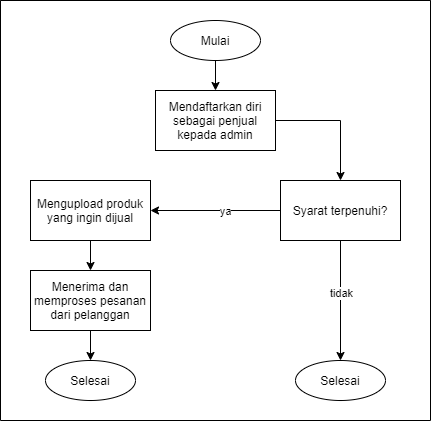
\includegraphics [width = 14cm, height= 10cm]{gambar/bisnis_diagram}}
		\caption{Business Diagram}
		\label{bisnis_diagram}
		\end{figure}

		Gambar 4.2 memperlihatkan alur bisnis di dalam sistem. Dimulai ketika pengguna ingin mendaftarkan diri sebagai penjual kepada admin dan kemudian admin meminta email yang valid dari penjual sebagai syarat untuk didaftarkan di sistem. Setelah syaratnya terpenuhi dan penjual sudah didaftarkan maka penjual harus memverifikasi emailnya tersebut, setelah terverifikasi maka proses bisnis selanjutnya adalah penjual menjual produknya di dalam sistem.
		Tahapan tersebut adalah tahapan yang sangat penting karena semakin banyak produk yang dijual maka akan semakin bervariasi pilihan produk yang dapat dipilih. Hal tersebut dapat menaikkan minat pengguna yang berperan sebagai pembeli untuk membeli produk dari sistem ini. Setelah pembeli membeli atau memesan produk, tahapan selanjutnya yang dapat dilakukan penjual adalah menerima pesanan tersebut serta memprosesnya.
	
	\item Activity Diagram
		\par Activity Diagram merupakan salah satu diagram yang termasuk ke dalam kategori behavioral UML. Activity Diagram akan menggambarkan langkah-langkah alur yang lebih rinci dari sistem yang merujuk pada Use case. Activity Diagram mempunyai titik mulai dan titik selesai yang di dalamnya menggambarkan berbagai alur kerja sistem secara beruntun. Biasanya Activity
		Diagram digunakan oleh pengembang aplikasi untuk memahami alur program yang akan dibuat. Berikut merupakan activity diagram dalam penelitian ini :

	\item Entity Relationship Diagram
		\par \textit{Entity Relationship Diagram} (ERD) merupakan diagram yang menjelaskan hubungan antar data-data yang ada disistem yang saling berelasi satu sama yang lain.
		\textit{Entity Relationship Diagram} (ERD) dapat dilihat pada Gambar \ref{erd}.

		\begin{figure}[H]
			\centering
			{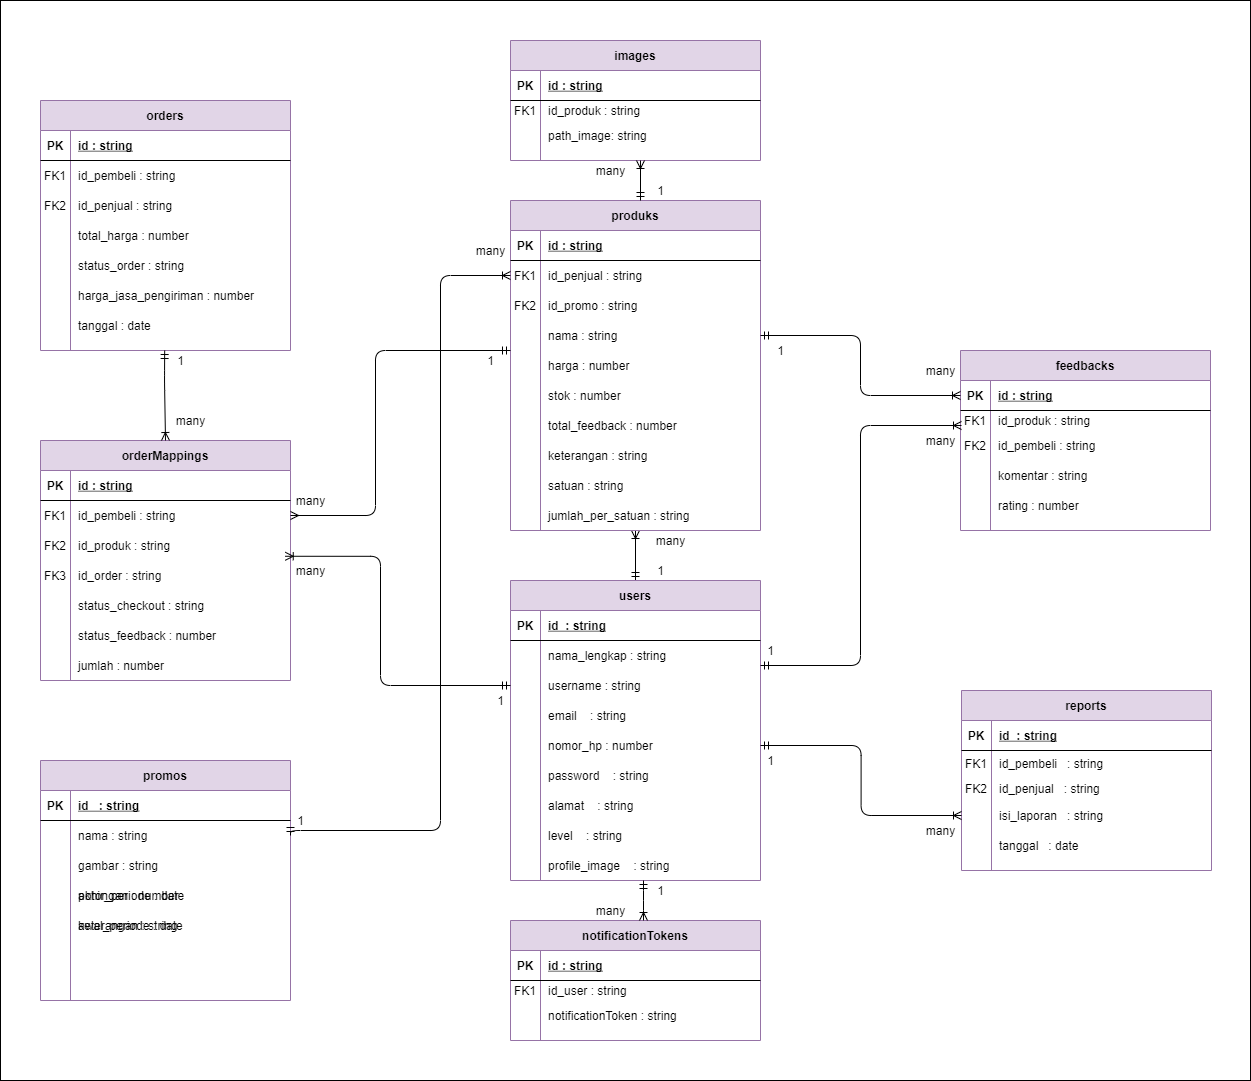
\includegraphics [width = 14cm, height= 10cm]{gambar/erd}}
			\caption{Entity Relationship Diagram}
			\label{erd}
		\end{figure}

		Gambar 4.3 menggambarkan relasi antar entitas di dalam sistem. Terdapat total 9 entitas di dalam sistem. Tiap relasi dari entitas memiliki kardinalitas (derajat).Derajat yang terlihat pada gambar 4.4 adalah derajat satu ke banyak. Derajat tersebut akan menunjukkan batas maksimum suatu entitas dapat berelasi dengan entitas lainnya. Adapun 9 entitas tersebut yang terdiri dari :

		\begin{enumerate}
			\item Entitas users
			\par Entitas ini akan menyimpan data semua pengguna di dalam aplikasi. Pada
			entitas users terdapat 9 atribut yaitu : id, nama-lengkap, username, email,
			nomor-hp, password, alamat, level, dan profile-image . Atribut id akan
			menjadi primary key serta di dalam entitas ini tidak memiliki foreign key.
			\item Entitas notificationTokens
			\par Entitas ini akan menyimpan data token ketika pengguna masuk ke dalam
			aplikasi berbasis android. Pada entitas notificationTokens terdapat 3 atribut
			yaitu : id, notificationToken, dan id-user . Atribut id akan menjadi primary
			key serta id-user dari entitas users akan menjadi foreign key.
			\item Entitas produks
			\par Entitas ini akan menyimpan data produk yang akan ditambahkan oleh penjual. Pada entitas produks terdapat 11 atribut yaitu : id, id-penjual, id-promo, nama, harga, stok, total-feedback, keterangan, satuan, jumlah-per-satuan. Atribut id akan menjadi primary key serta id-penjual dari entitas users dan id-promo dari entitas promos akan menjadi foreign key.
			\item Entitas images
			\par Entitas ini akan menyimpan data yang berupa gambar dari entitas produks dikarenakan satu data produk dapat memiliki lebih dari satu gambar. Pada
			entitas images terdapat 3 atribut yaitu : id, id-produk dan path-image . Atribut id akan menjadi primary key serta id-produk dari entitas produks akan menjadi foreign key.
			\item Entitas promos
			\par Entitas ini akan menyimpan data promo yang akan digunakan ketika suatu produk memiliki potongan harga atau promo. Pada entitas promos terdapat 5 atribut yaitu : id, nama, gambar, potongan, awal-periode, akhir-periode, dan
			keterangan . Atribut id akan menjadi primary key serta di dalam entitas ini tidak memiliki foreign key apapun.
			\item Entitas orderMappings
			\par Entitas ini akan menyimpan data setiap produk yang dipilih oleh pembeli ketika pembeli memesan produk atau melakukan checkout di dalam aplikasi berbasis android. Pada entitas orderMappings terdapat 7 atribut yaitu : id, id-pembeli,
			id-produk, id-order, status-checkout, status-feedback, dan jumlah. Atribut id
			akan menjadi primary key serta id-pembeli dari entitas users, id-produk dari entitas produks dan id-order dari entitas orders akan menjadi foreign key.
			\item Entitas orders
			\par Entitas ini akan menyimpan data pesanan pembeli yang berasal dari entitas orderMappings. Pada entitas orders terdapat 7 atribut yaitu : id, id-pembeli, id-penjual, total-harga, status-order, harga-jasa-pengiriman, dan tanggal. Atribut id akan menjadi primary key serta id-pembeli dan id-penjual dari entitas users akan menjadi foreign key.
			\item Entitas feedbacks
			\par Entitas ini akan menyimpan data ulasan setiap produk yang diberikan oleh pembeli. Pada entitas feedbacks terdapat 5 atribut yaitu : id, id-produk,
			id-pembeli, komentar, dan rating. Atribut id akan menjadi primary key serta id-pembeli dari entitas users dan id-produk dari entitas produks akan menjadi foreign key.
			\item Entitas reports
			\par Entitas ini akan menyimpan data laporan tentang penjual yang dilakukan oleh pembeli. Pada entitas reports terdapat 5 atribut yaitu : id, id-penjual, id-pembeli, isi-laporan, dan tanggal. Atribut id akan menjadi primary key serta id-pembeli dan id-penjual dari entitas users akan menjadi foreign key.
		\end{enumerate}
	
	\item Antarmuka Aplikasi
	\par Antarmuka dalam aplikasi berbasis web ini terdiri dari bagian admin dan bagian penjual. Dikarenakan terdapat beberapa perbedaan fitur aplikasi sesuai dengan jenis penggunanya.

		\begin{enumerate}
			\item Antarmuka Aplikasi Bagian Admin
			\par Dapat dilihat pada gambar 4.21, ketika pertama kali mengakses aplikasi web melalui browser, maka akan muncul halaman home kemudian apabila admin ingin masuk kedalam aplikasi dapat menklik tombol masuk yang ada dipojok kanan atas.

			\begin{figure}[H]
				\centering
				{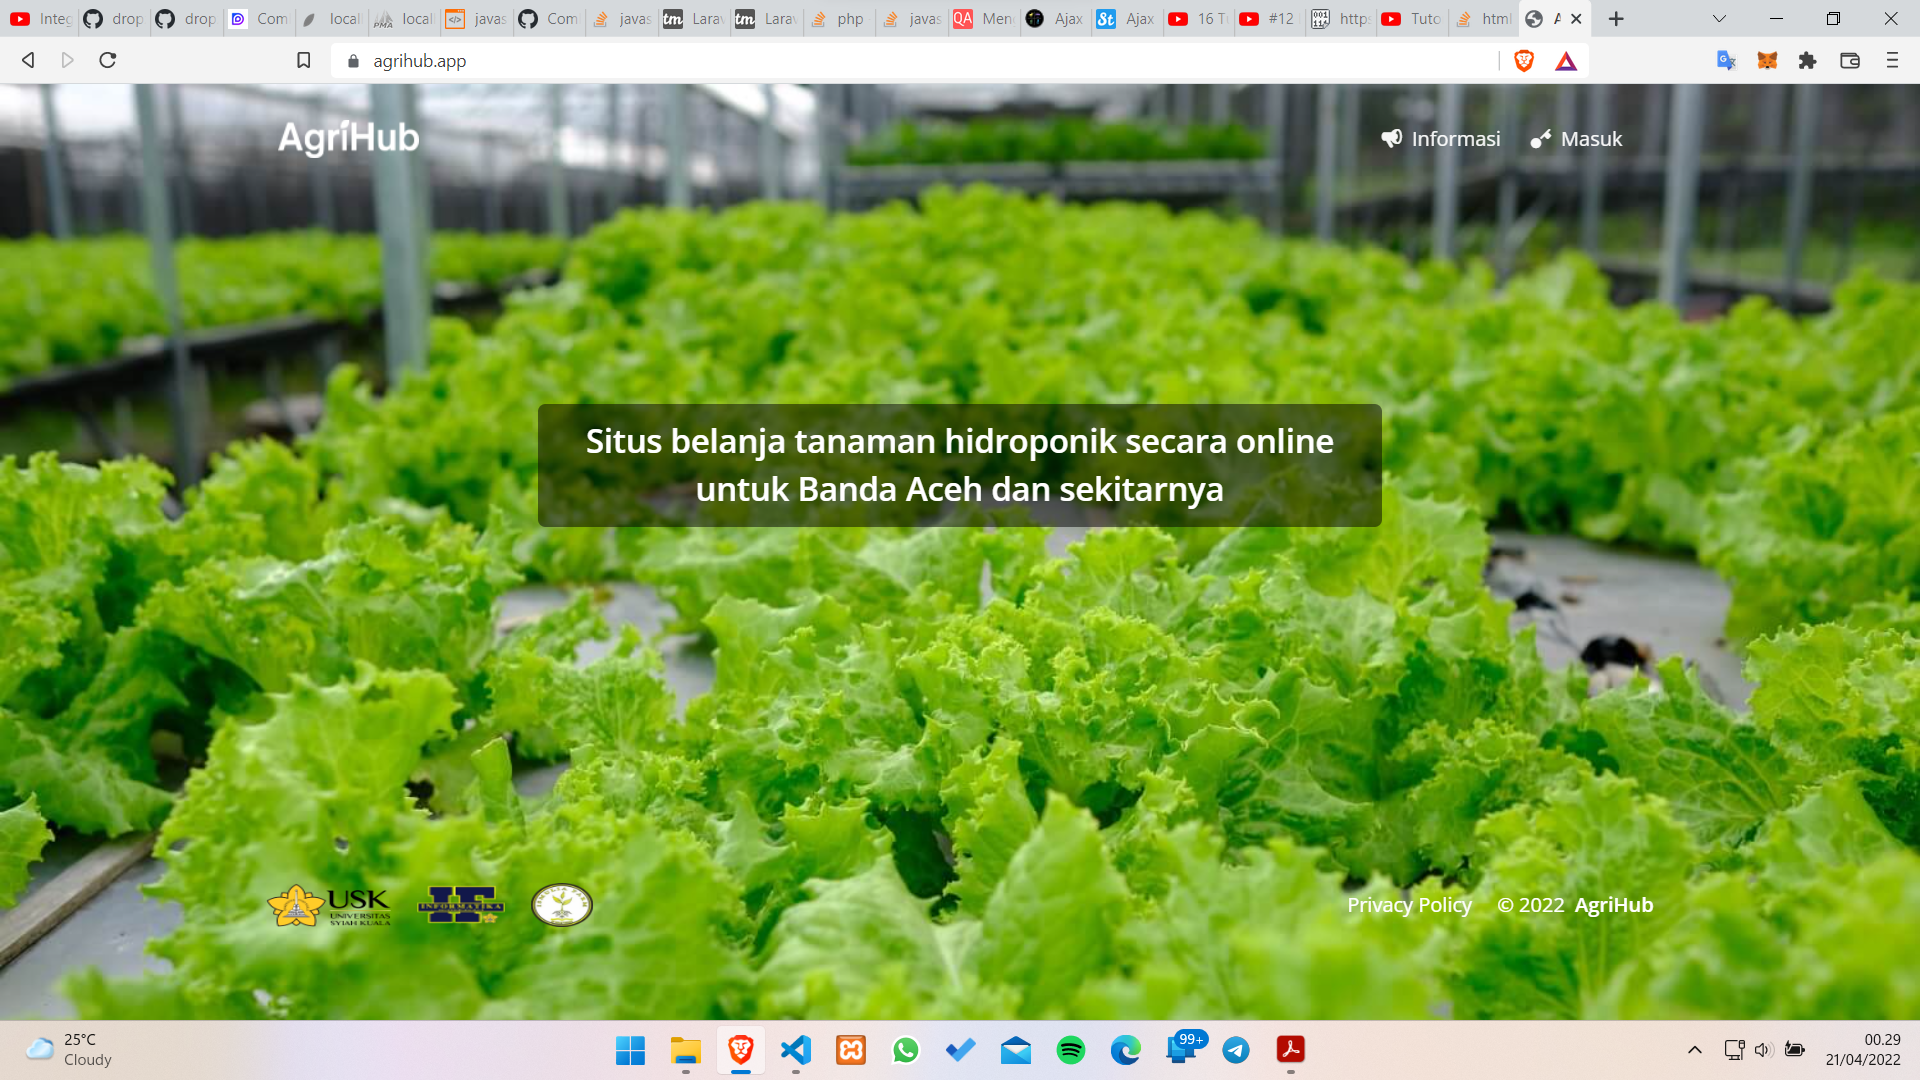
\includegraphics [width = 14.3cm, height= 9cm]{gambar/homepage}}
				\caption{Halaman Home}
				\label{homepage}
			\end{figure}

			\par Setelah menklik tombol masuk maka akan muncul tampilan untuk mengisi email dan password seperti gambar 4.5, apabila admin sudah mengisi email dan password maka dapat menekan tombol masuk yang berwarna hijau untuk masuk kedalam aplikasinya.

			\begin{figure}[H]
				\centering
				{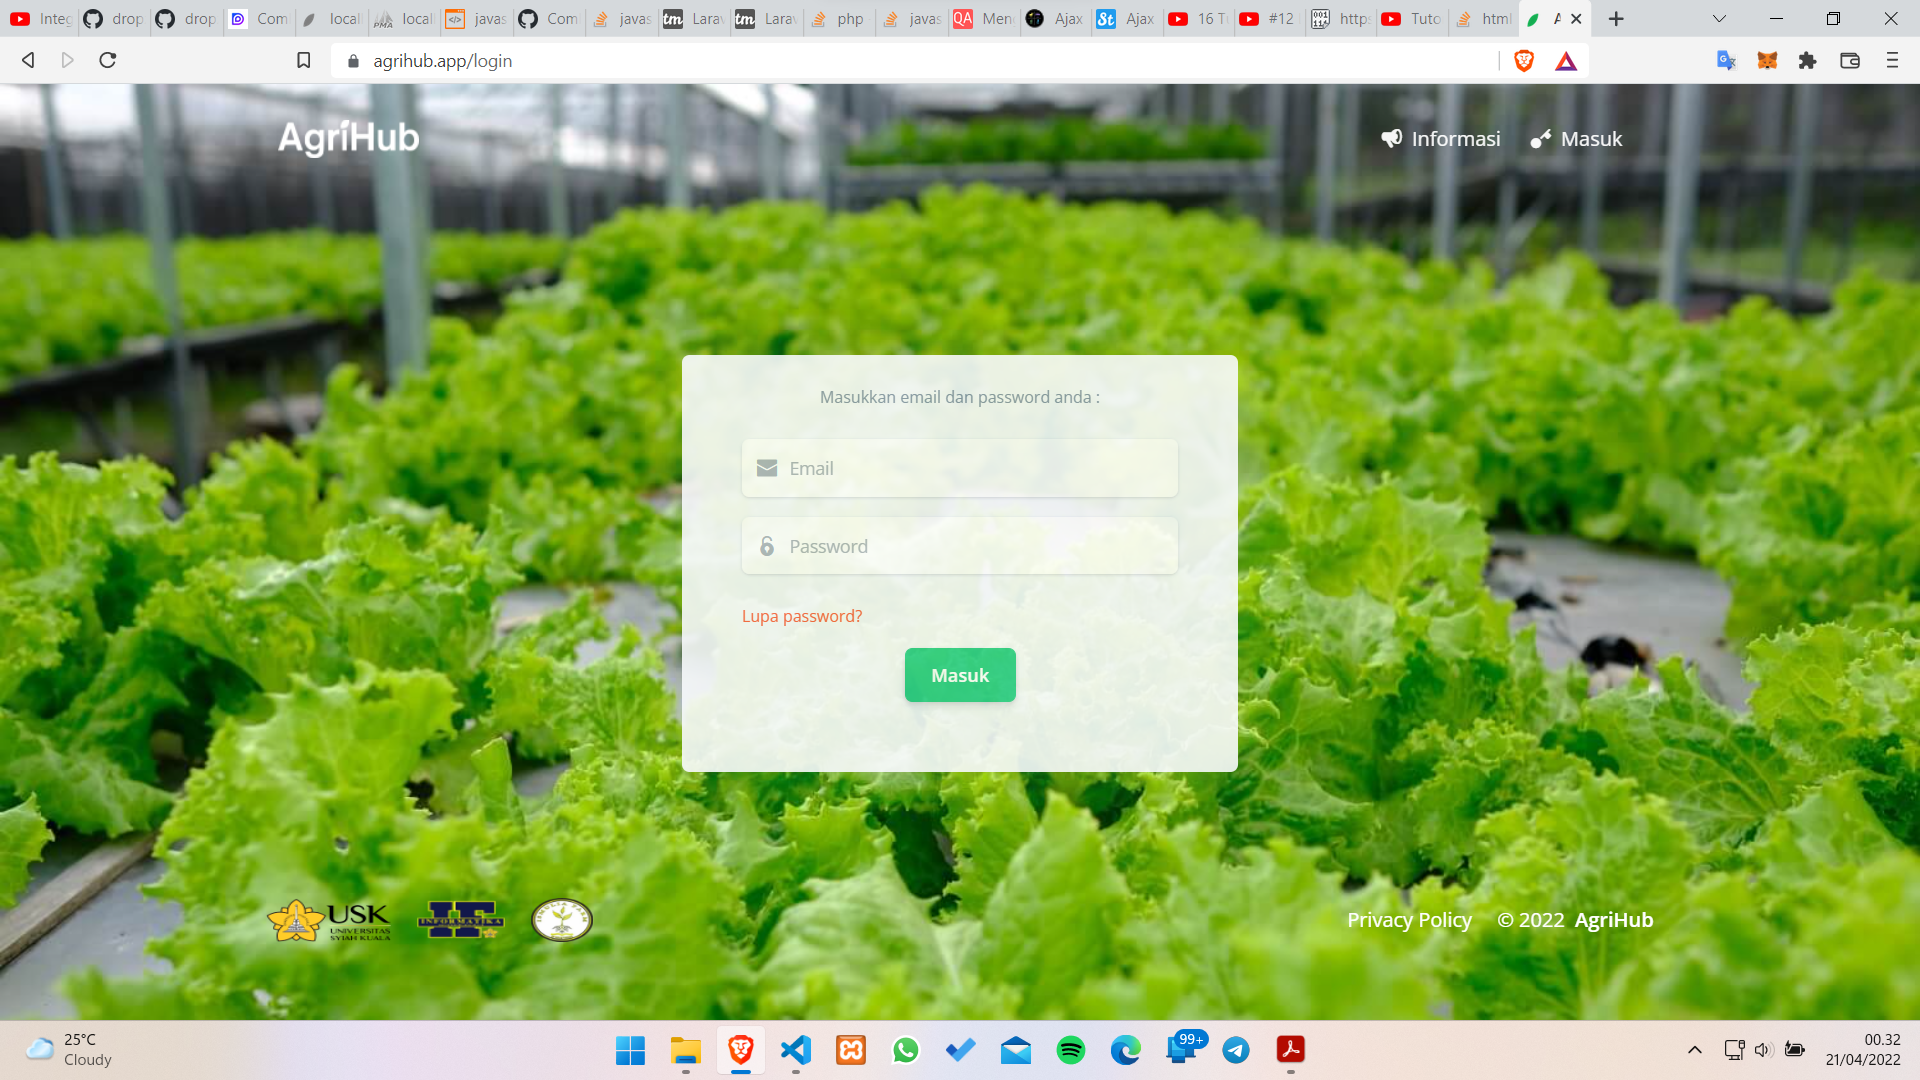
\includegraphics [width = 14.3cm, height= 9cm]{gambar/login}}
				\caption{Halaman Login}
				\label{login}
			\end{figure}

			\par Apabila admin lupa passwordnya maka dapat menekan tombol lupa password yang berwarna merah kemudian mengisikan email yang terdaftar untuk dikirimkan email reset passwordnya.

			\begin{figure}[H]
				\centering
				{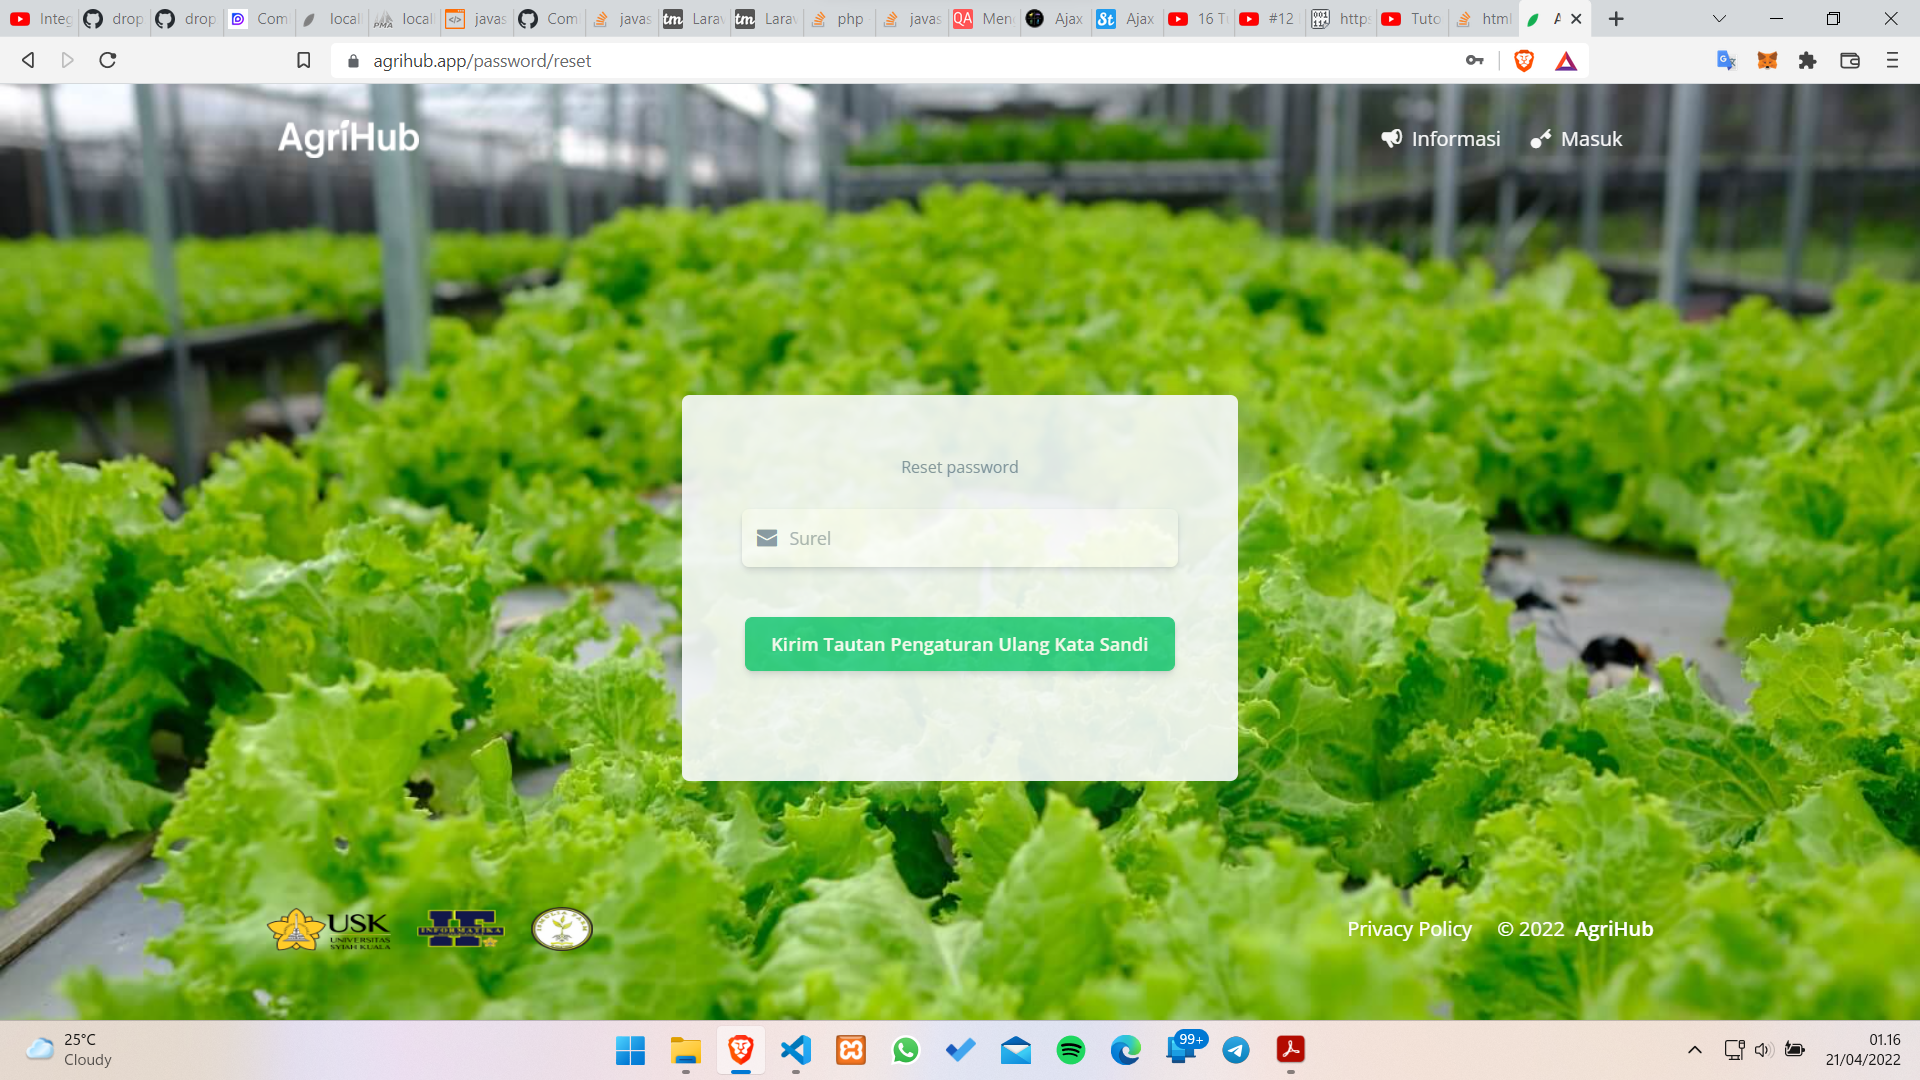
\includegraphics [width = 14.3cm, height= 9cm]{gambar/lupa_password}}
				\caption{Halaman Lupa Password}
				\label{lupa_password}
			\end{figure}

			\par Setelah berhasil masuk kedalam aplikasi maka akan disuguhkan tampilan dashboard yang berisi informasi mengenai data aplikasi AgriHub seperti jumlah produk yang sudah diupload oleh para penjual, jumlah pesenan yang sudah terjadi diaplikasi, jumlah promo yang sedang berlangsung, jumlah pengguna yang sudah terdaftar diaplikasi, jumlah laporan yang masuk dari pembeli, serta jumlah ulasan yang sudah diberikan oleh pembeli terhadap produk yang dijual oleh penjual. Dan juga ditampilkan grafik jumlah pesanan selesai dan batal perbulan dari para penjual selama 6 bulan terakhir, dan grafik jumlah produk baru yang diupload oleh para penjual selama 6 bulan terakhir serta grafik jumlah admin, penjual dan pembeli.

			\begin{figure}[H]
				\centering
				{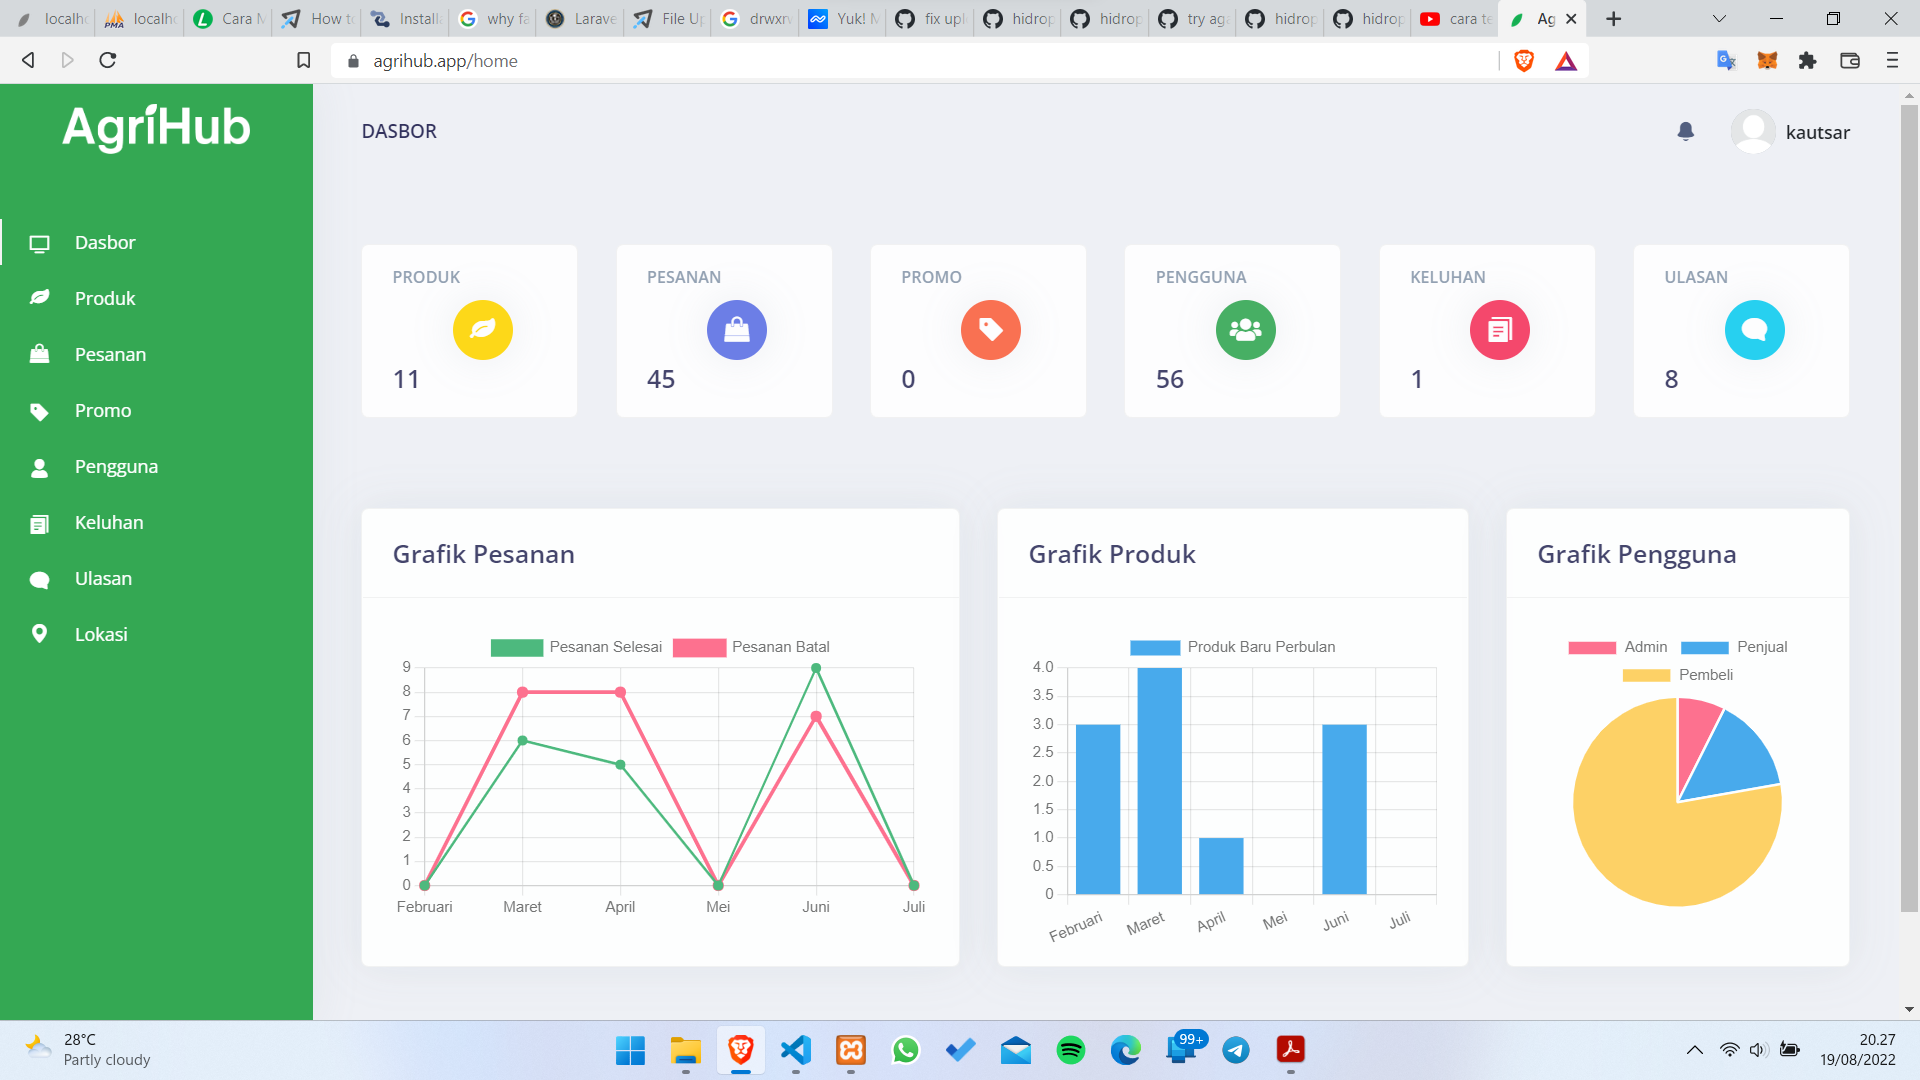
\includegraphics [width = 14.3cm, height= 9cm]{gambar/admin/dashboard_admin}}
				\caption{Halaman Dashboard Admin}
				\label{dashboard_admin}
			\end{figure}

			Pada halaman produk admin dapat melihat daftar produk yang sudah diupload oleh para penjual. melihat keterangan produk dan gambar lainnya dari produk dengan menekan tombol lihat yang berwarna hijau.

			\begin{figure}[H]
				\centering
				{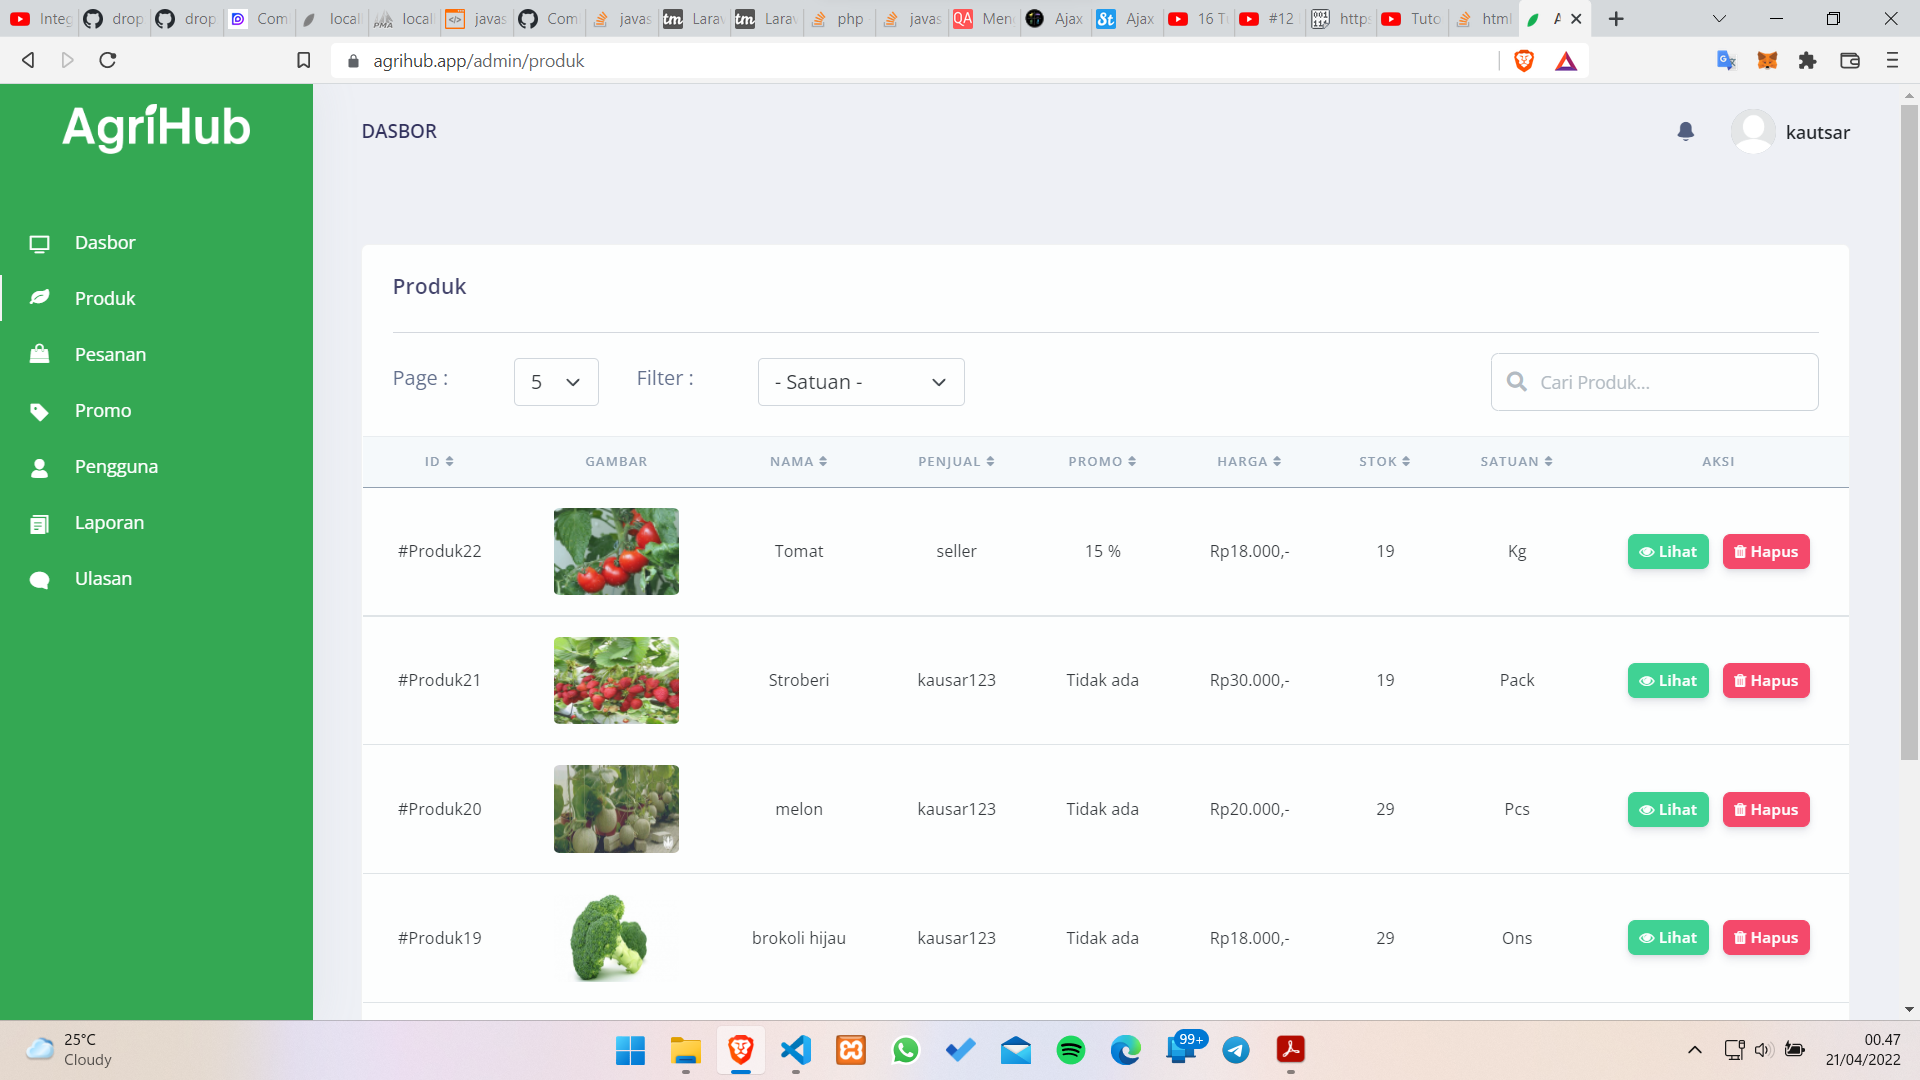
\includegraphics [width = 14.3cm, height= 9cm]{gambar/admin/produk_admin}}
				\caption{Halaman Produk Admin}
				\label{produk_admin}
			\end{figure}

			\par admin dapat melakukan pencarian produk tertentu dan dapat menghapusnya jika dianggap produknya asal-asalan.

			\begin{figure}[H]
				\centering
				{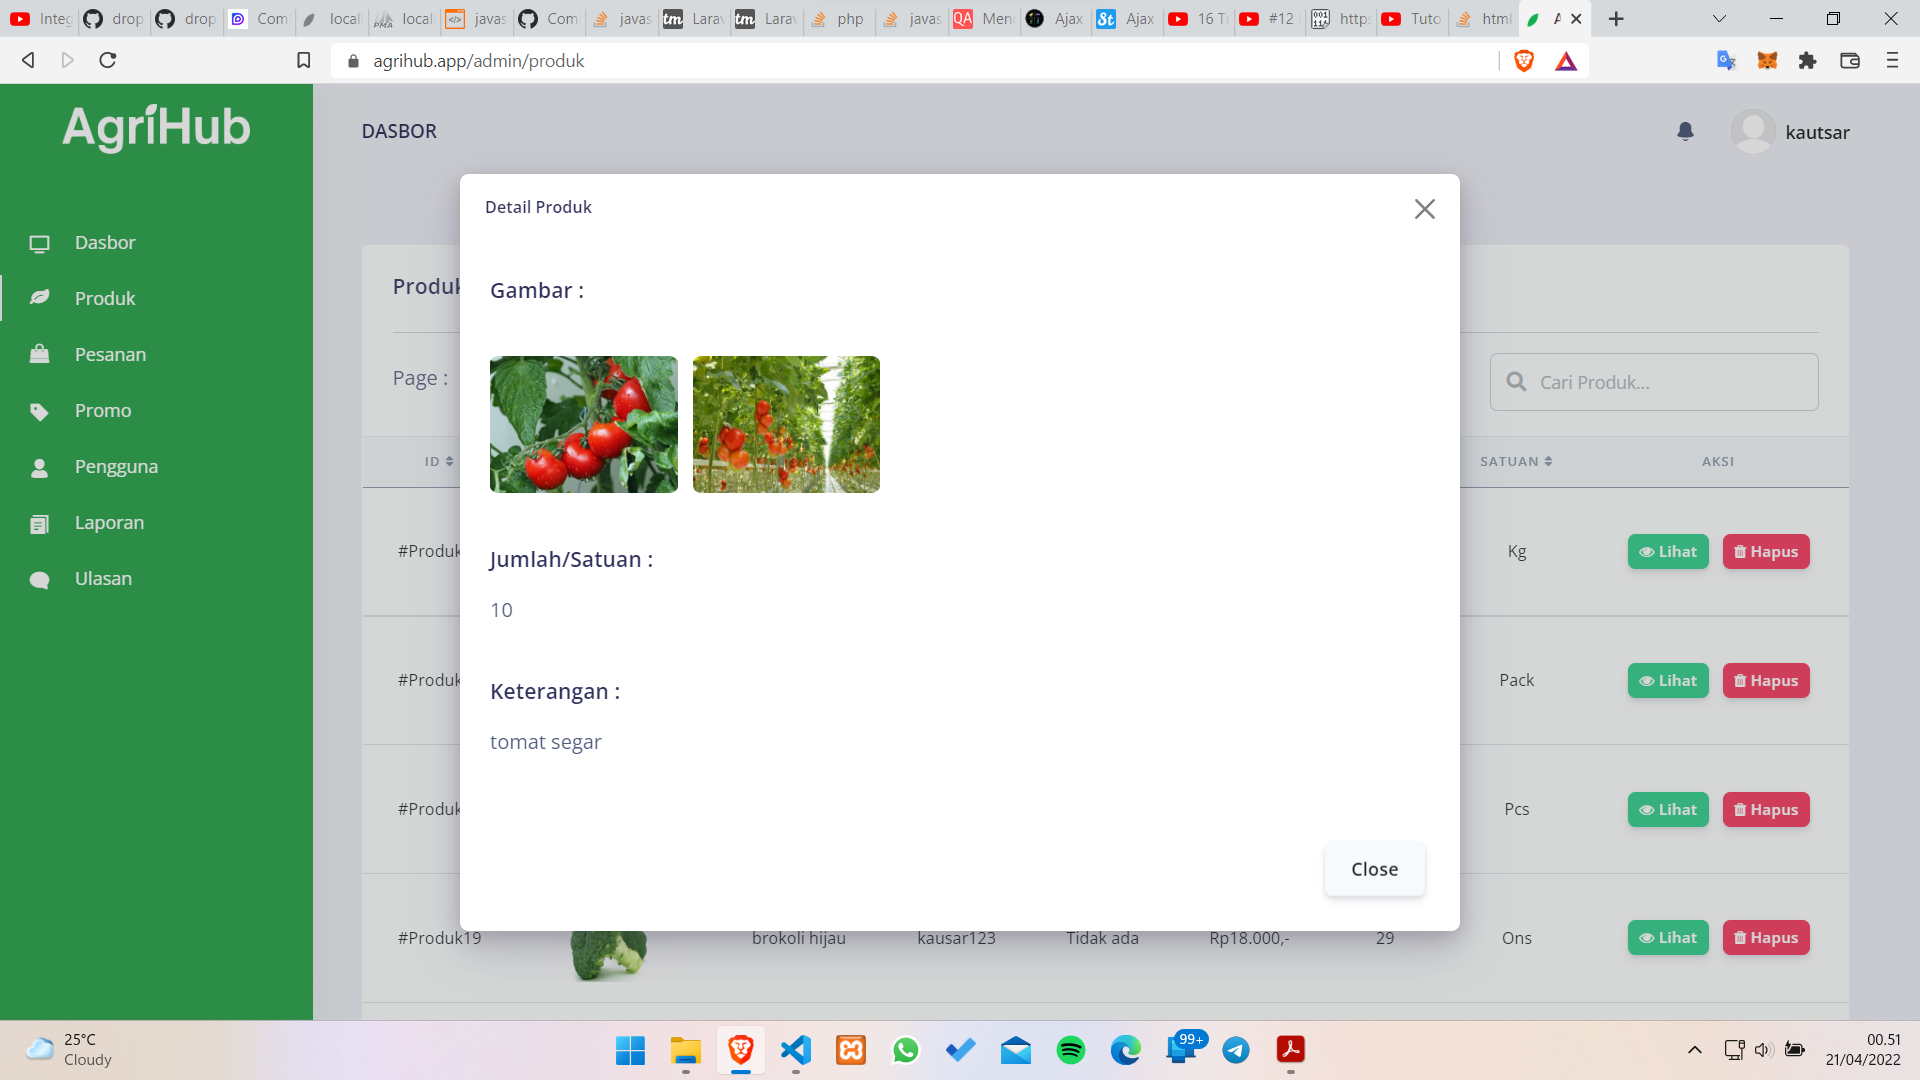
\includegraphics [width = 14.3cm, height= 9cm]{gambar/admin/lihat_produk_admin}}
				\caption{Halaman Lihat Produk Admin}
				\label{lihat_produk_admin}
			\end{figure}

			\begin{figure}[H]
				\centering
				{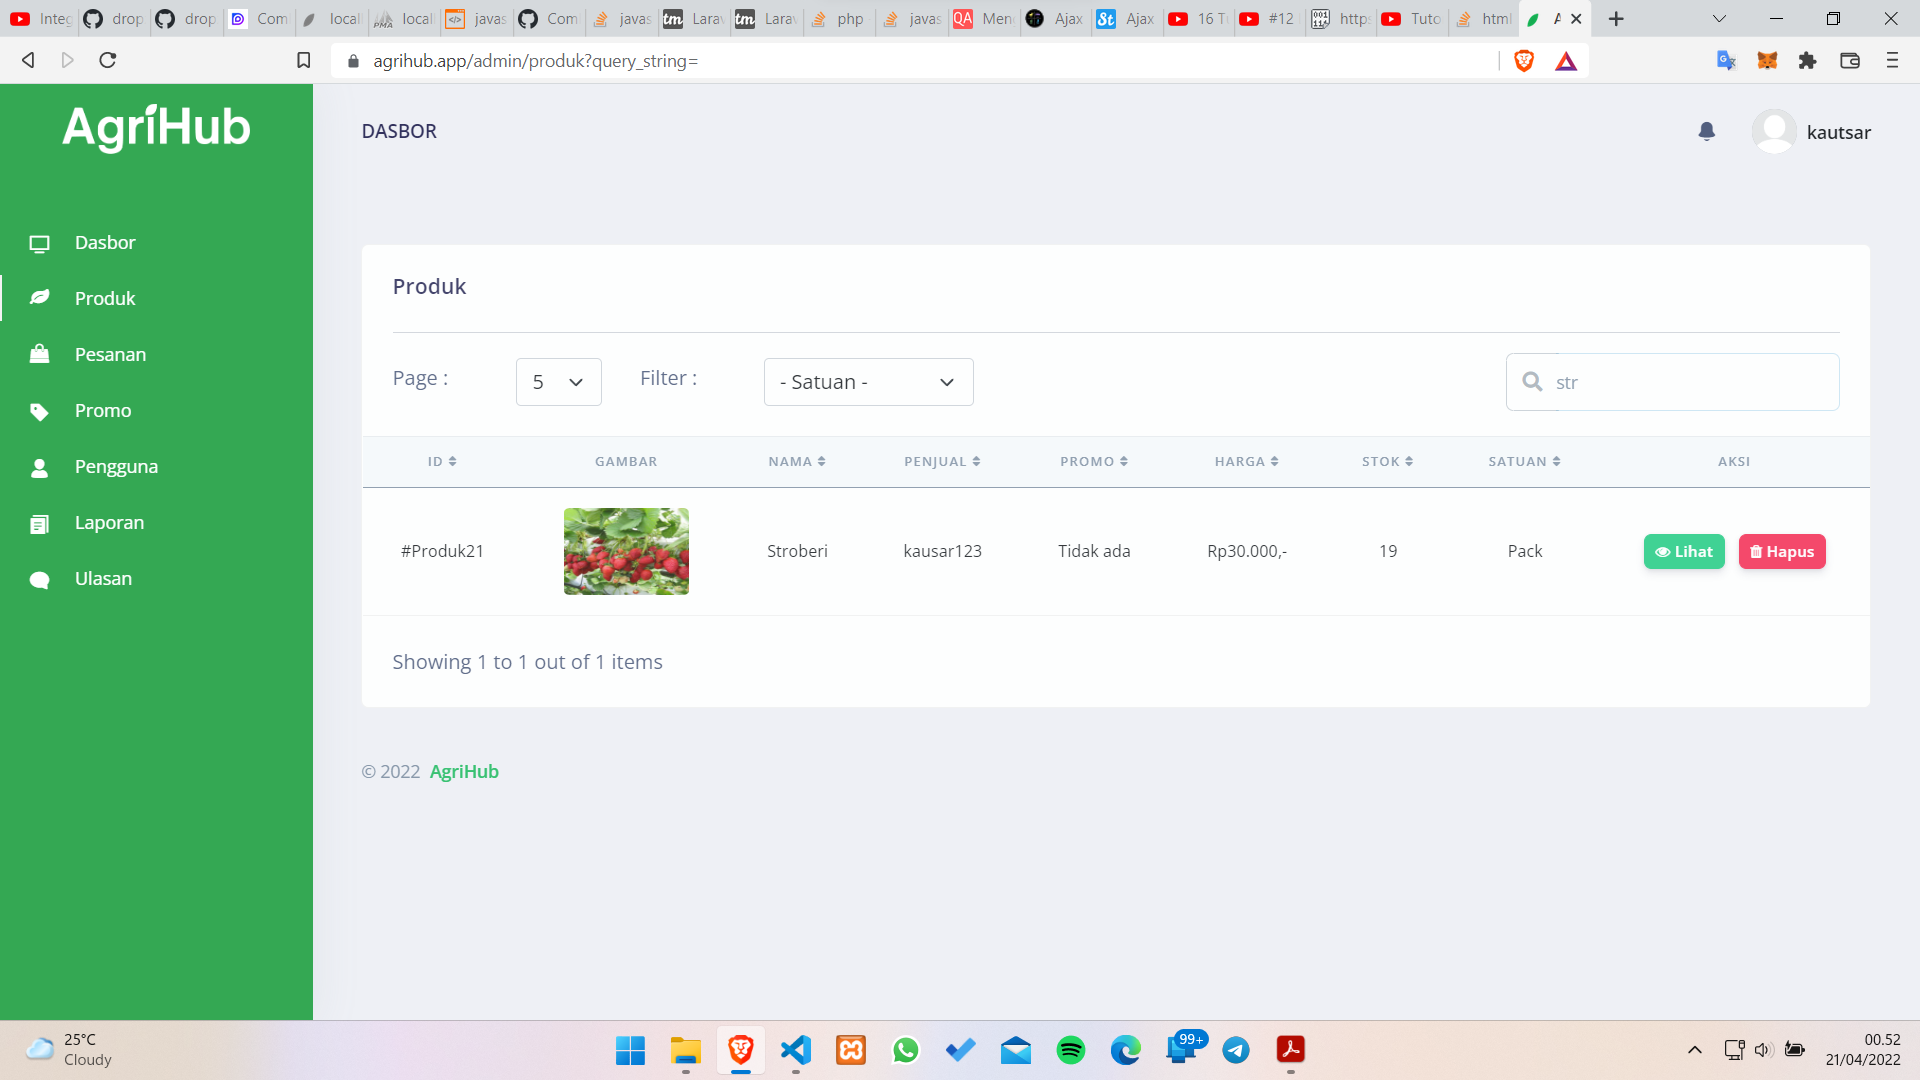
\includegraphics [width = 14.3cm, height= 9cm]{gambar/admin/pencarian_produk_admin}}
				\caption{Halaman Pencarian Produk Admin}
				\label{pencarian_produk_admin}
			\end{figure}

			\begin{figure}[H]
				\centering
				{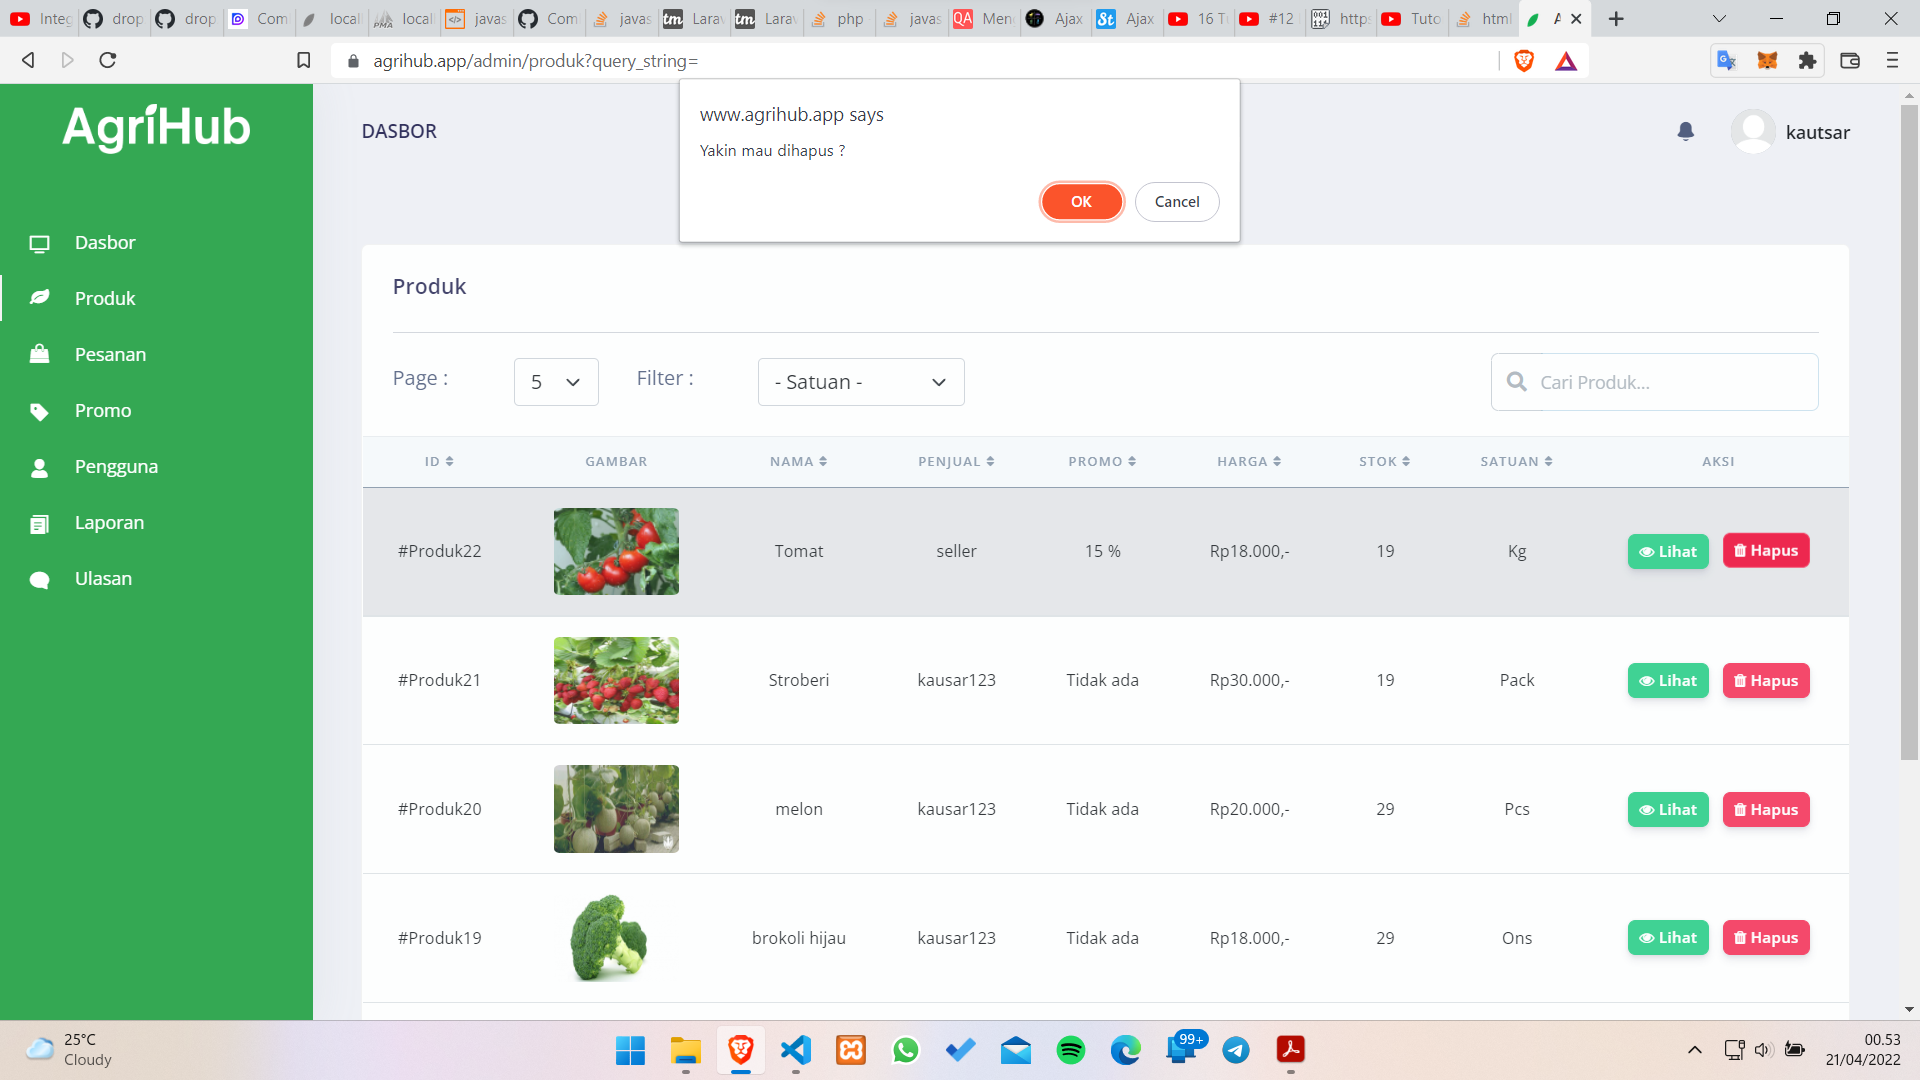
\includegraphics [width = 14.3cm, height= 9cm]{gambar/admin/hapus_produk_admin}}
				\caption{Halaman Hapus Produk Admin}
				\label{hapus_produk_admin}
			\end{figure}

			\par Pada menu pesanan admin dapat melihat semua pesanan yang sudah terjadi diaplikasi antara penjual dengan pembeli, dan juga dapat melihat detailnya dengan menekan tombol detail serta dapat mengekspornya dalam bentuk pdf jika diperlukan. dan dapat menfilter datanya berdasarkan status pesanannya seperti ingin melihat pesanan yang berstatus batal saja.

			\begin{figure}[H]
				\centering
				{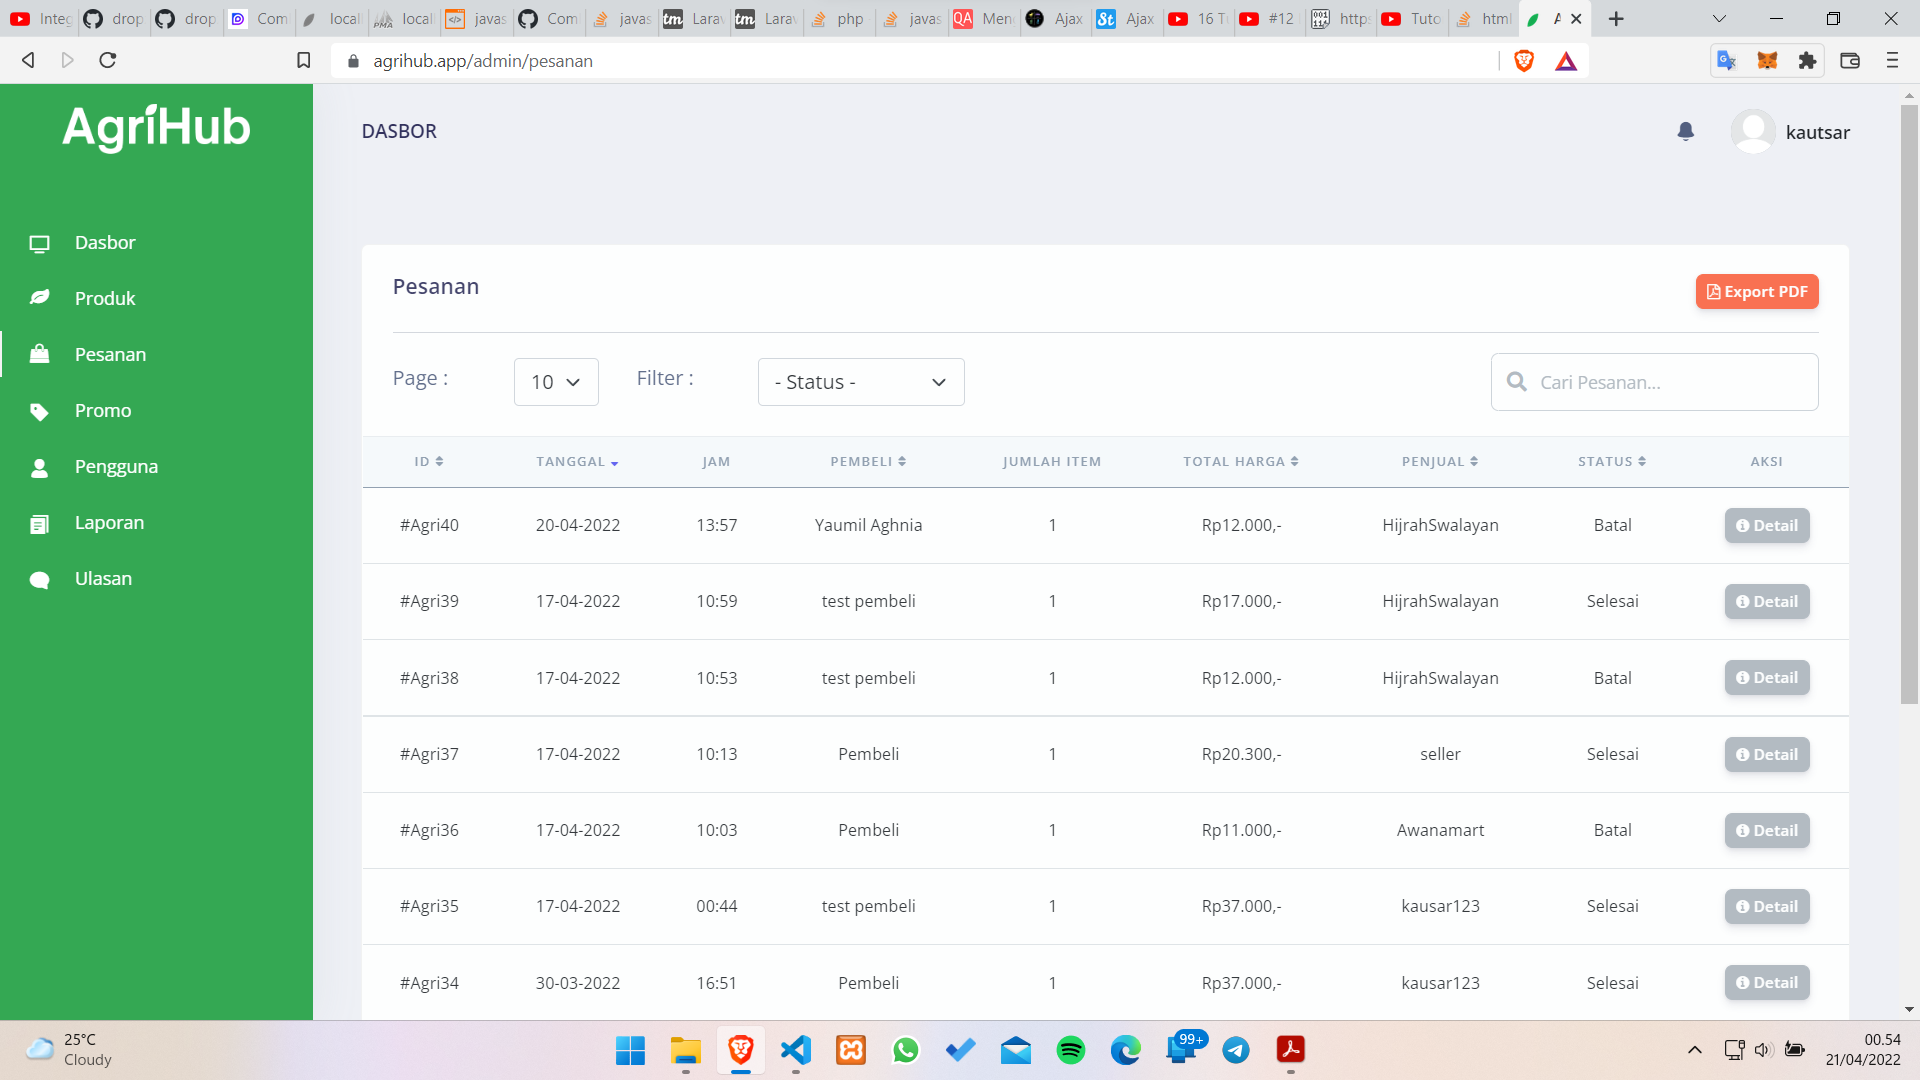
\includegraphics [width = 14.3cm, height= 9cm]{gambar/admin/pesanan_admin}}
				\caption{Halaman Pesanan Admin}
				\label{pesanan_admin}
			\end{figure}

			\begin{figure}[H]
				\centering
				{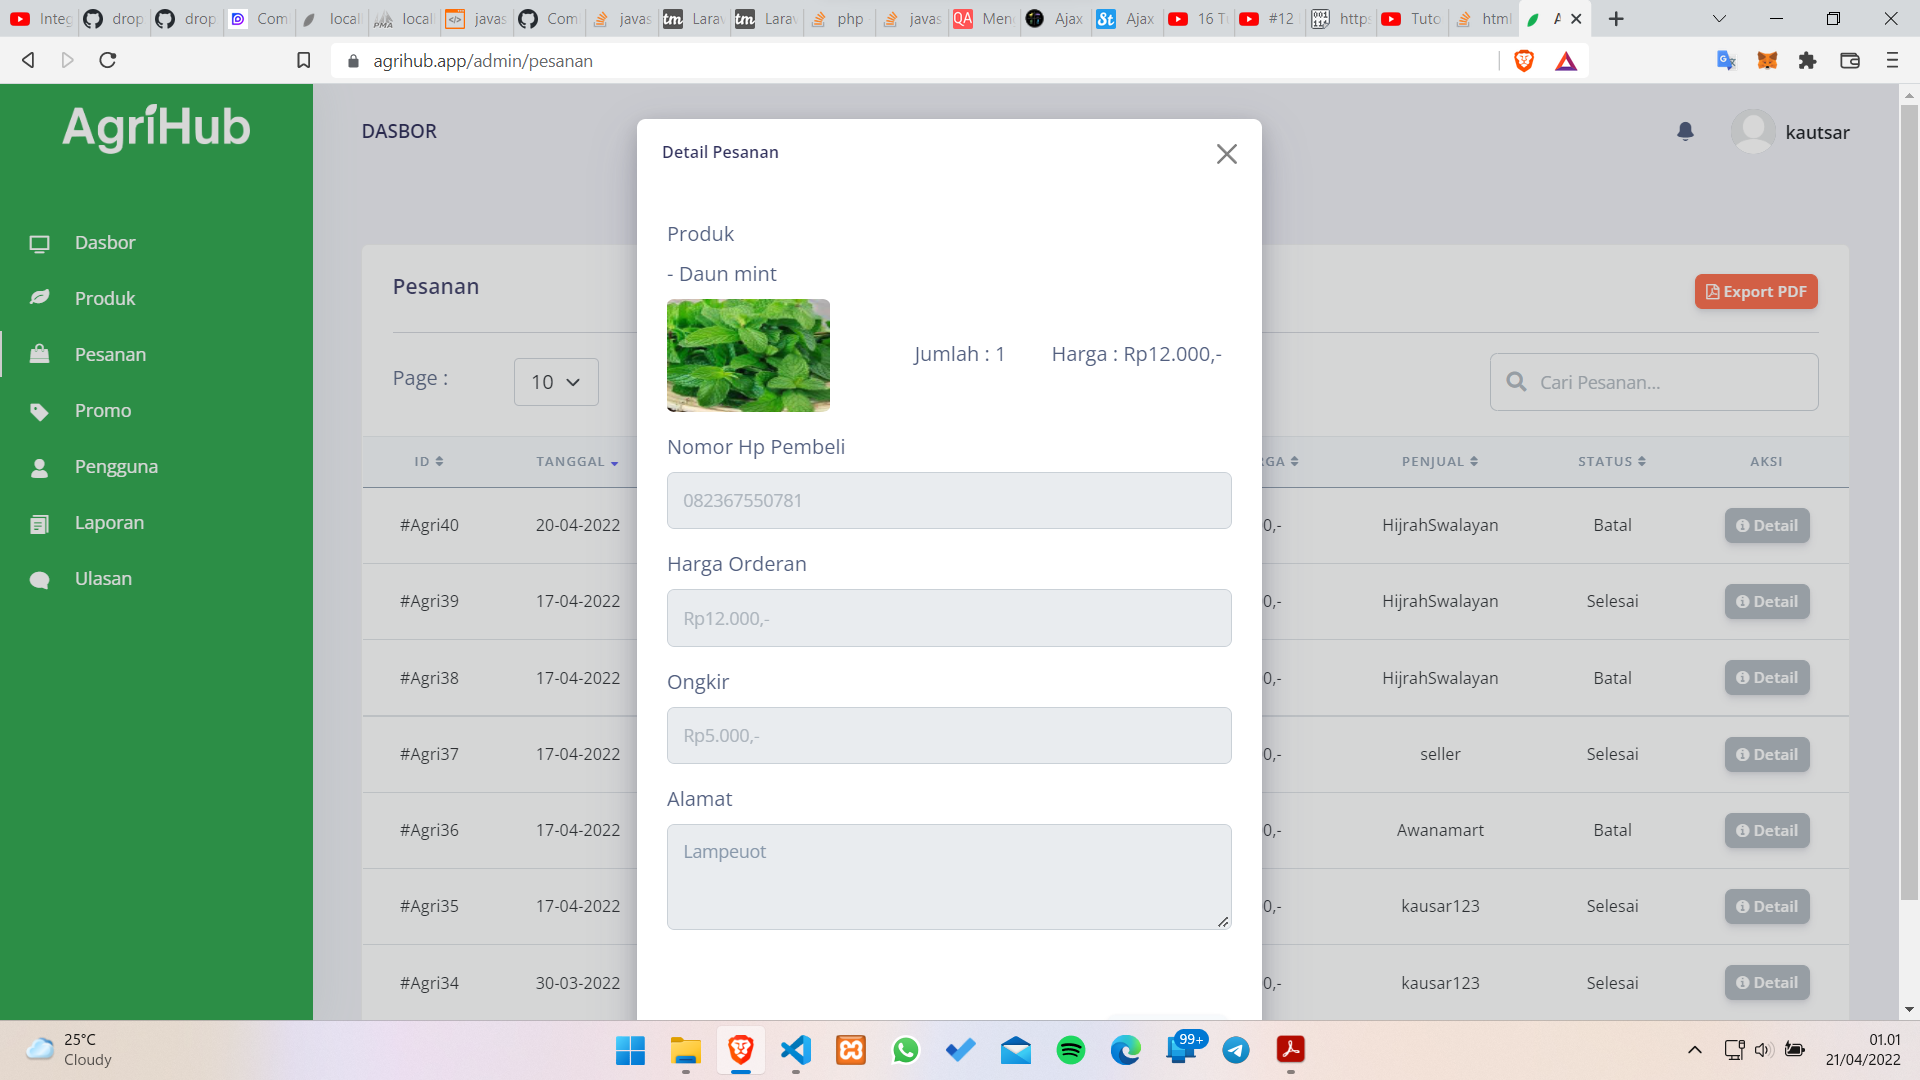
\includegraphics [width = 14.3cm, height= 9cm]{gambar/admin/detail_pesanan}}
				\caption{Halaman Detail Pesanan}
				\label{detail_pesanan}
			\end{figure}

			\begin{figure}[H]
				\centering
				{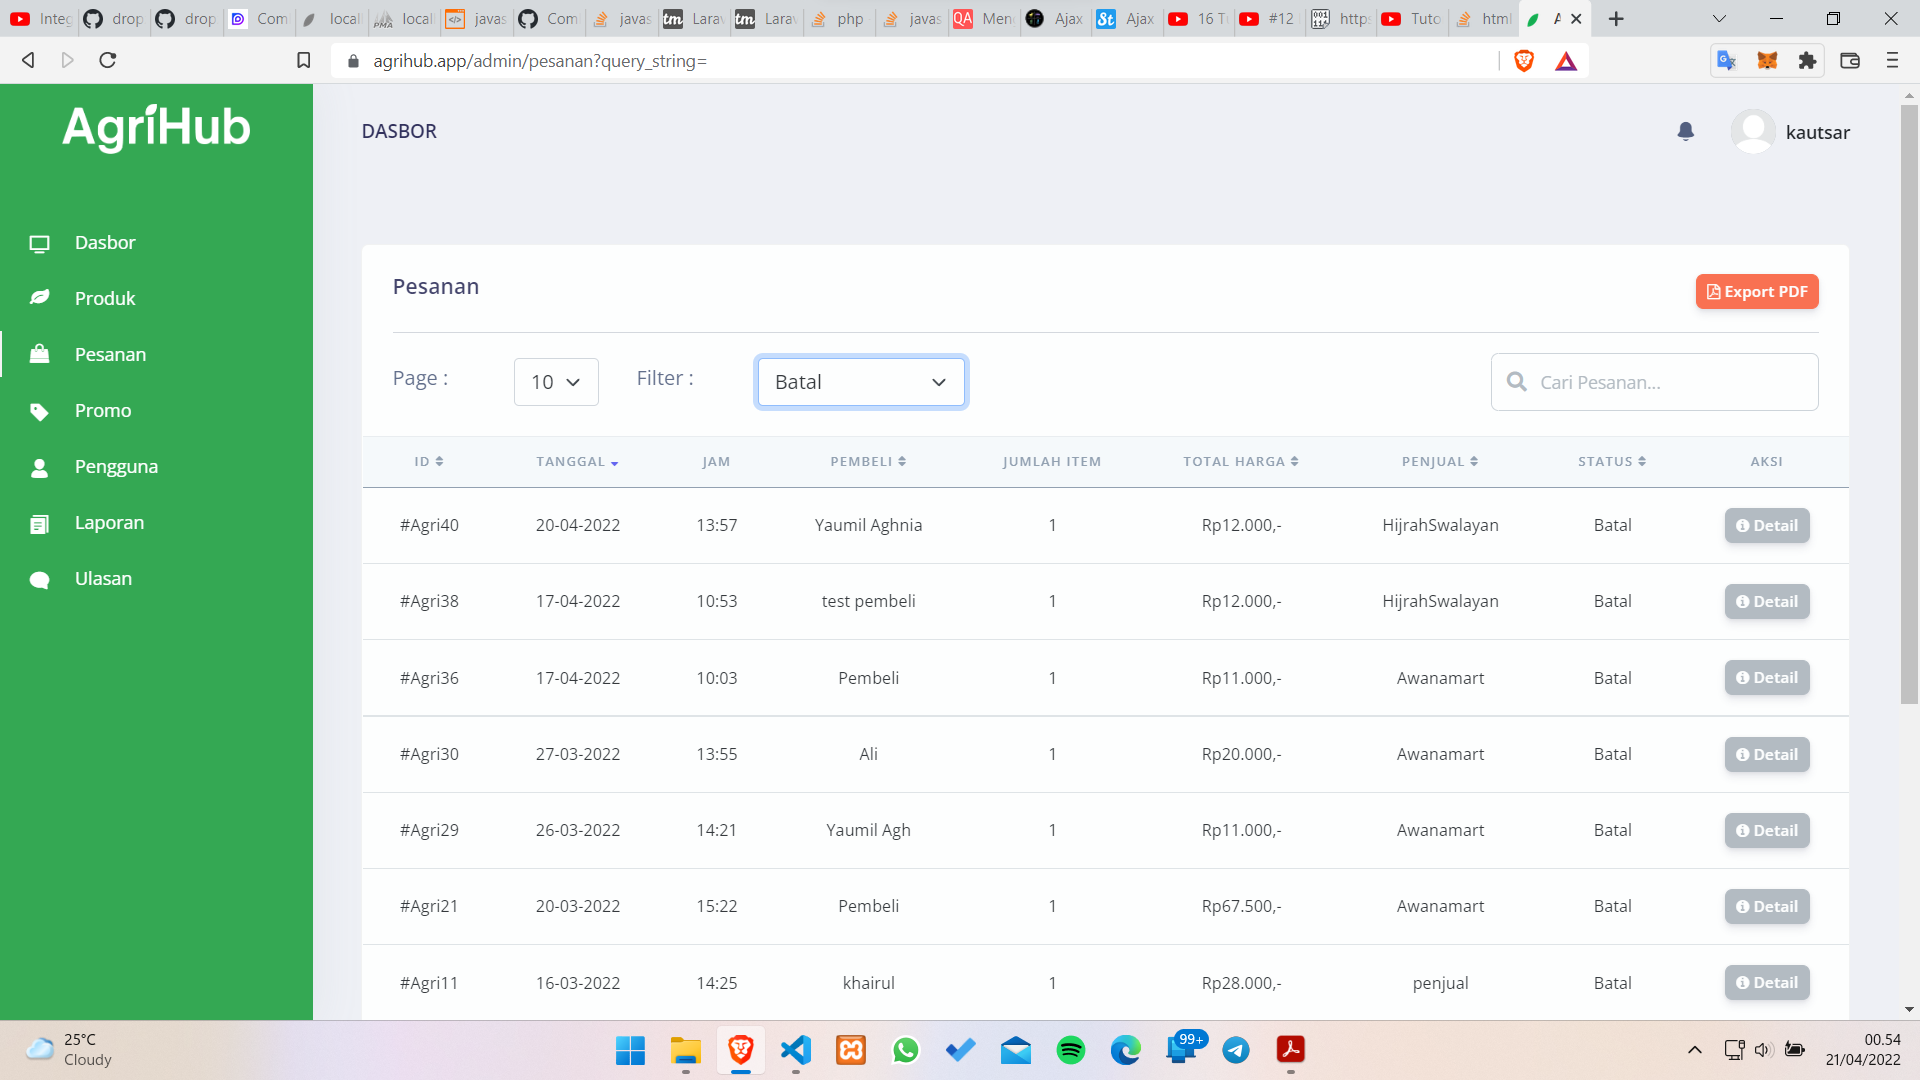
\includegraphics [width = 14.3cm, height= 9cm]{gambar/admin/filter_pesanan_admin}}
				\caption{Halaman Filter Pesanan Admin}
				\label{filter_pesanan_admin}
			\end{figure}

			\begin{figure}[H]
				\centering
				{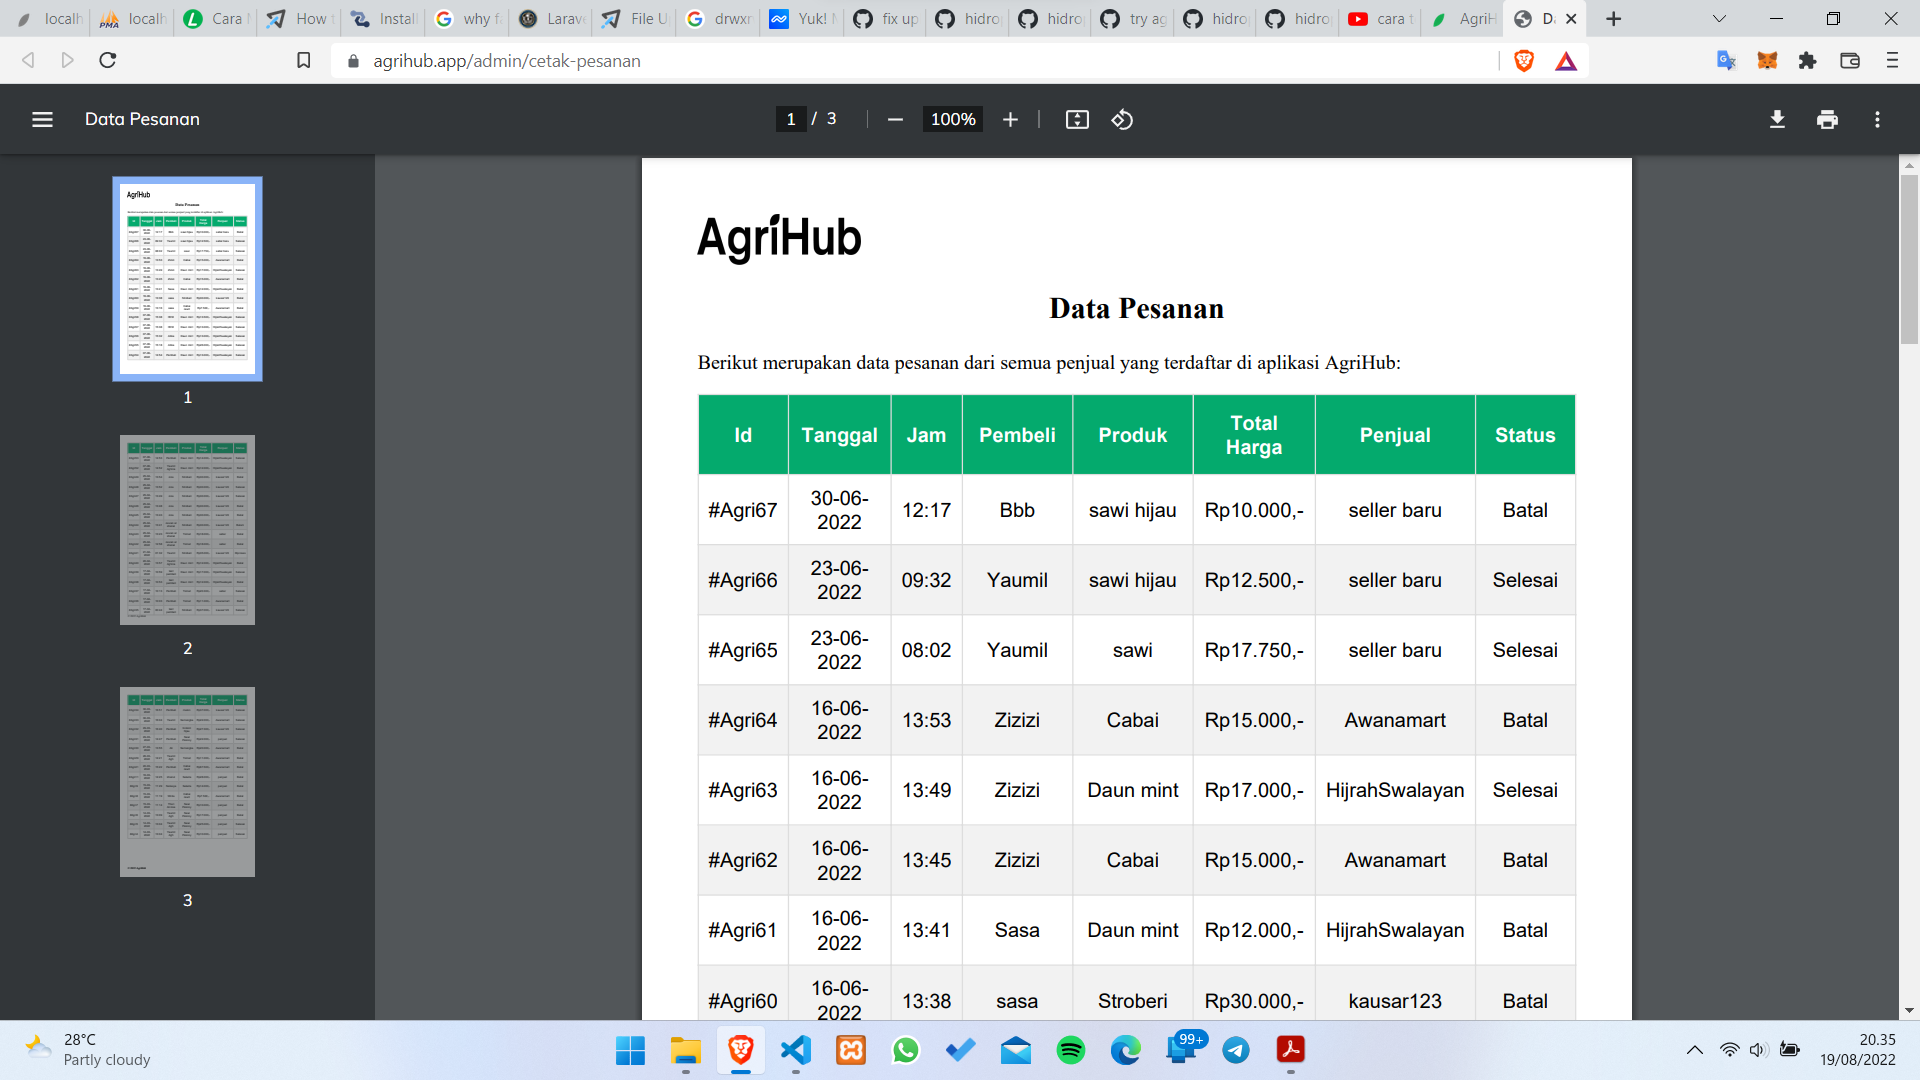
\includegraphics [width = 14.3cm, height= 9cm]{gambar/admin/export_pesanan_admin}}
				\caption{Halaman Export Pesanan Admin}
				\label{export_pesanan_admin}
			\end{figure}

			\par Pada halaman promo ini admin dapat menambahkan promo baru kedalam aplikasi sehingga nantinya dapat digunakan oleh para penjual.

			\begin{figure}[H]
				\centering
				{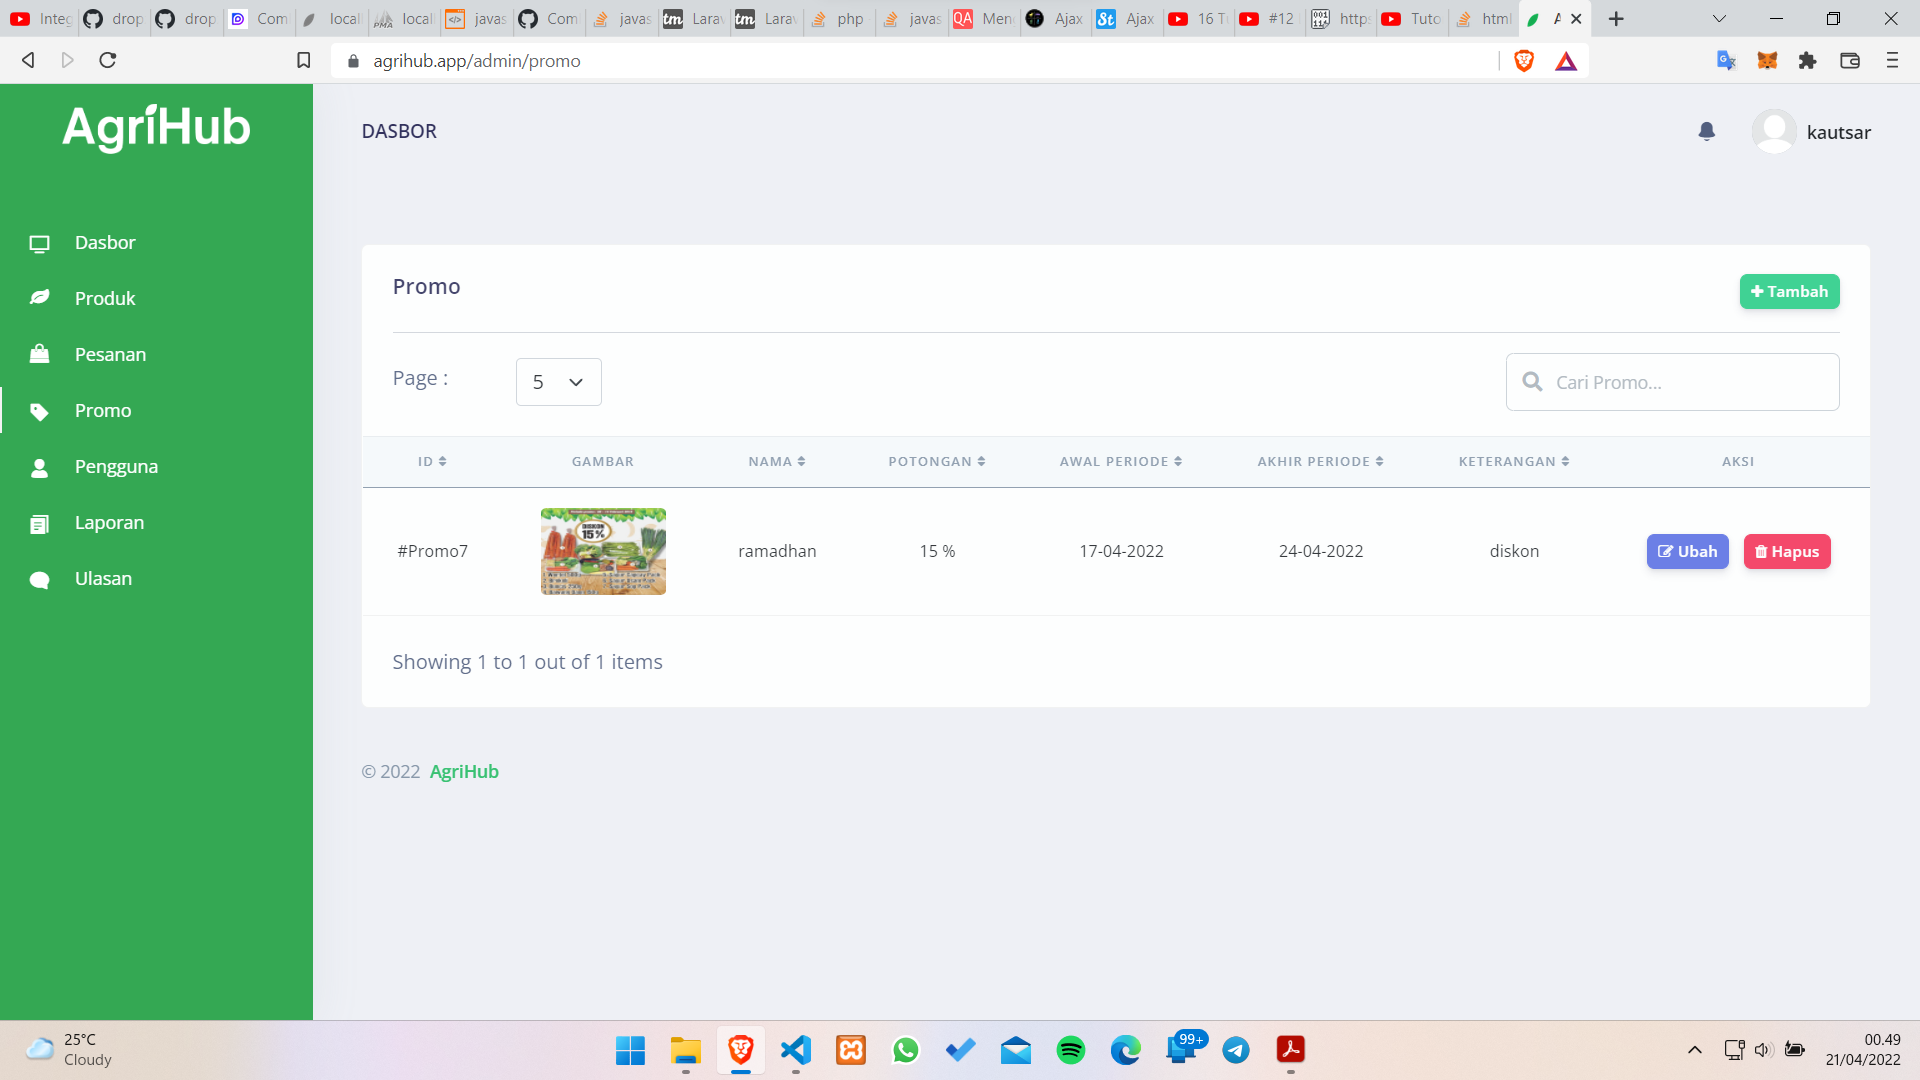
\includegraphics [width = 14.3cm, height= 9cm]{gambar/admin/promo}}
				\caption{Halaman Promo Admin}
				\label{promo}
			\end{figure}

			\begin{figure}[H]
				\centering
				{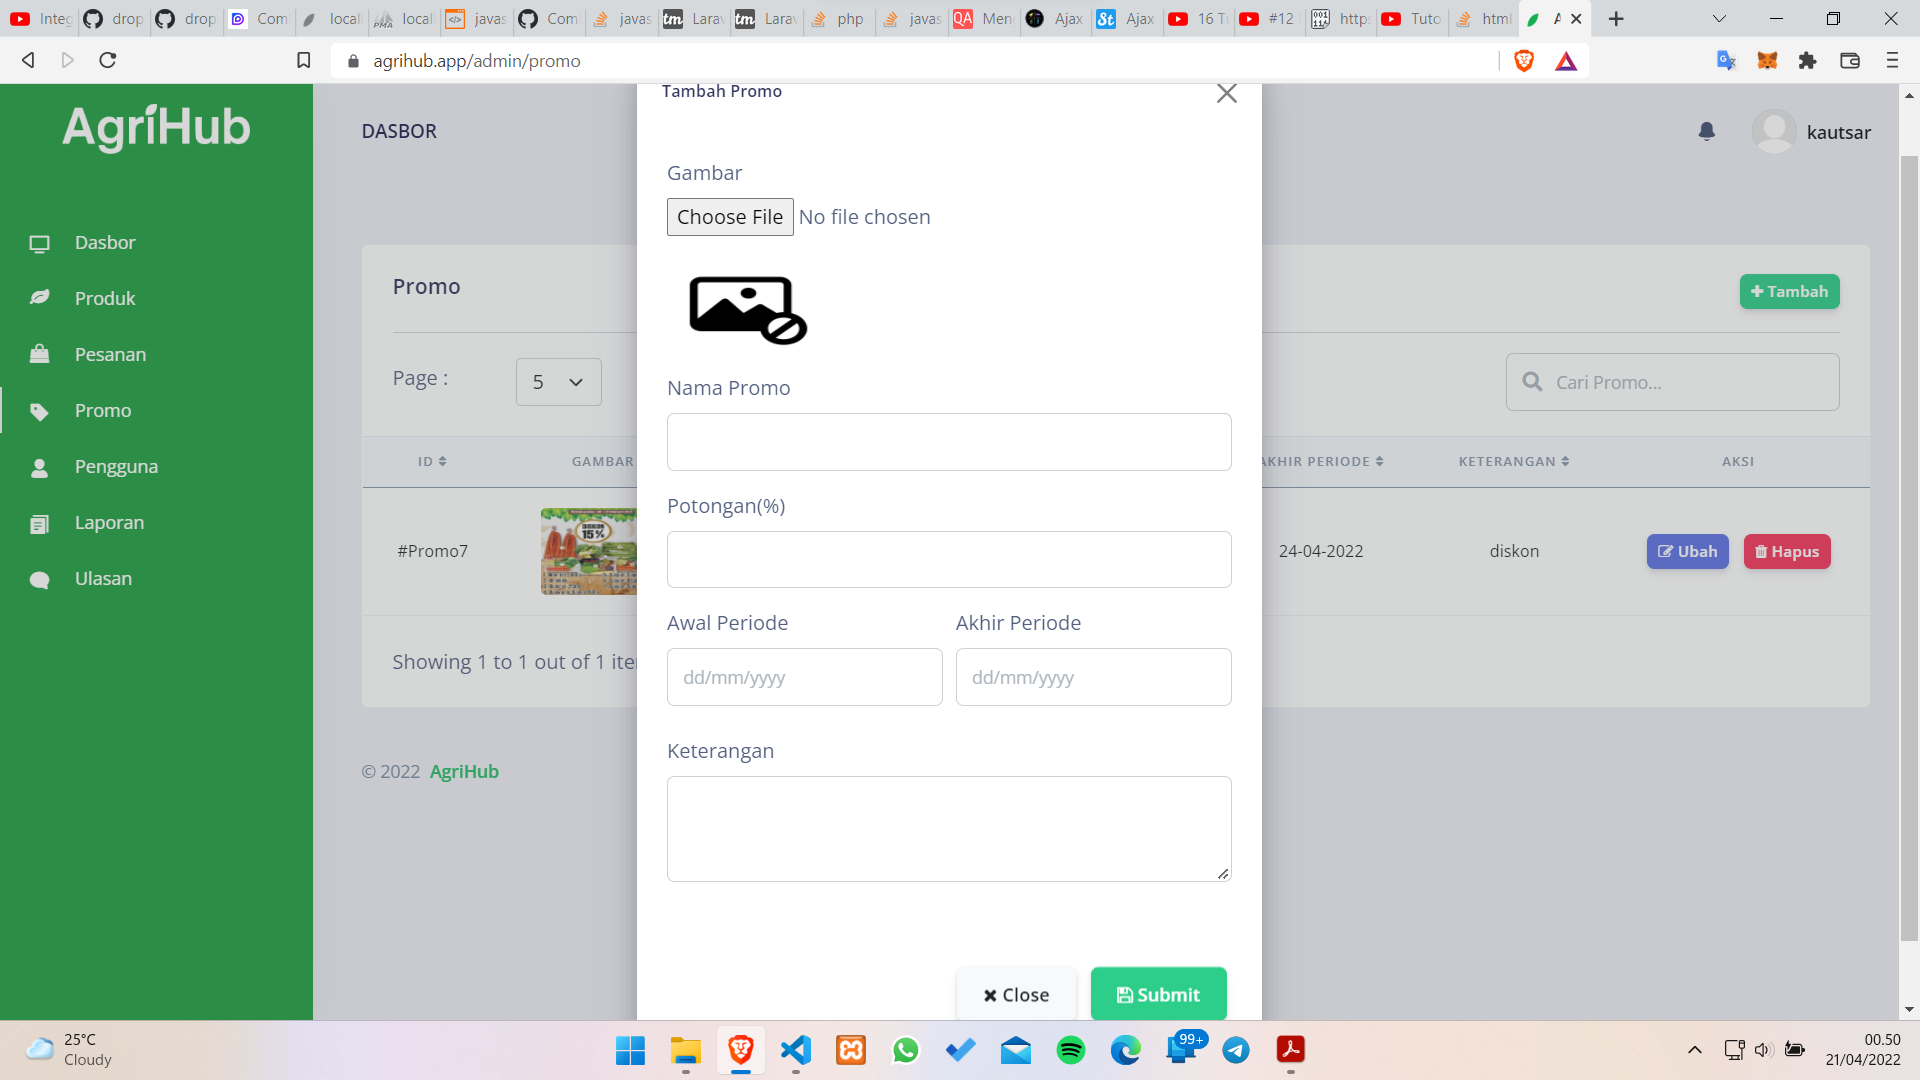
\includegraphics [width = 14.3cm, height= 9cm]{gambar/admin/tambah_promo}}
				\caption{Halaman Tambah Promo}
				\label{tambah_promo}
			\end{figure}

			\begin{figure}[H]
				\centering
				{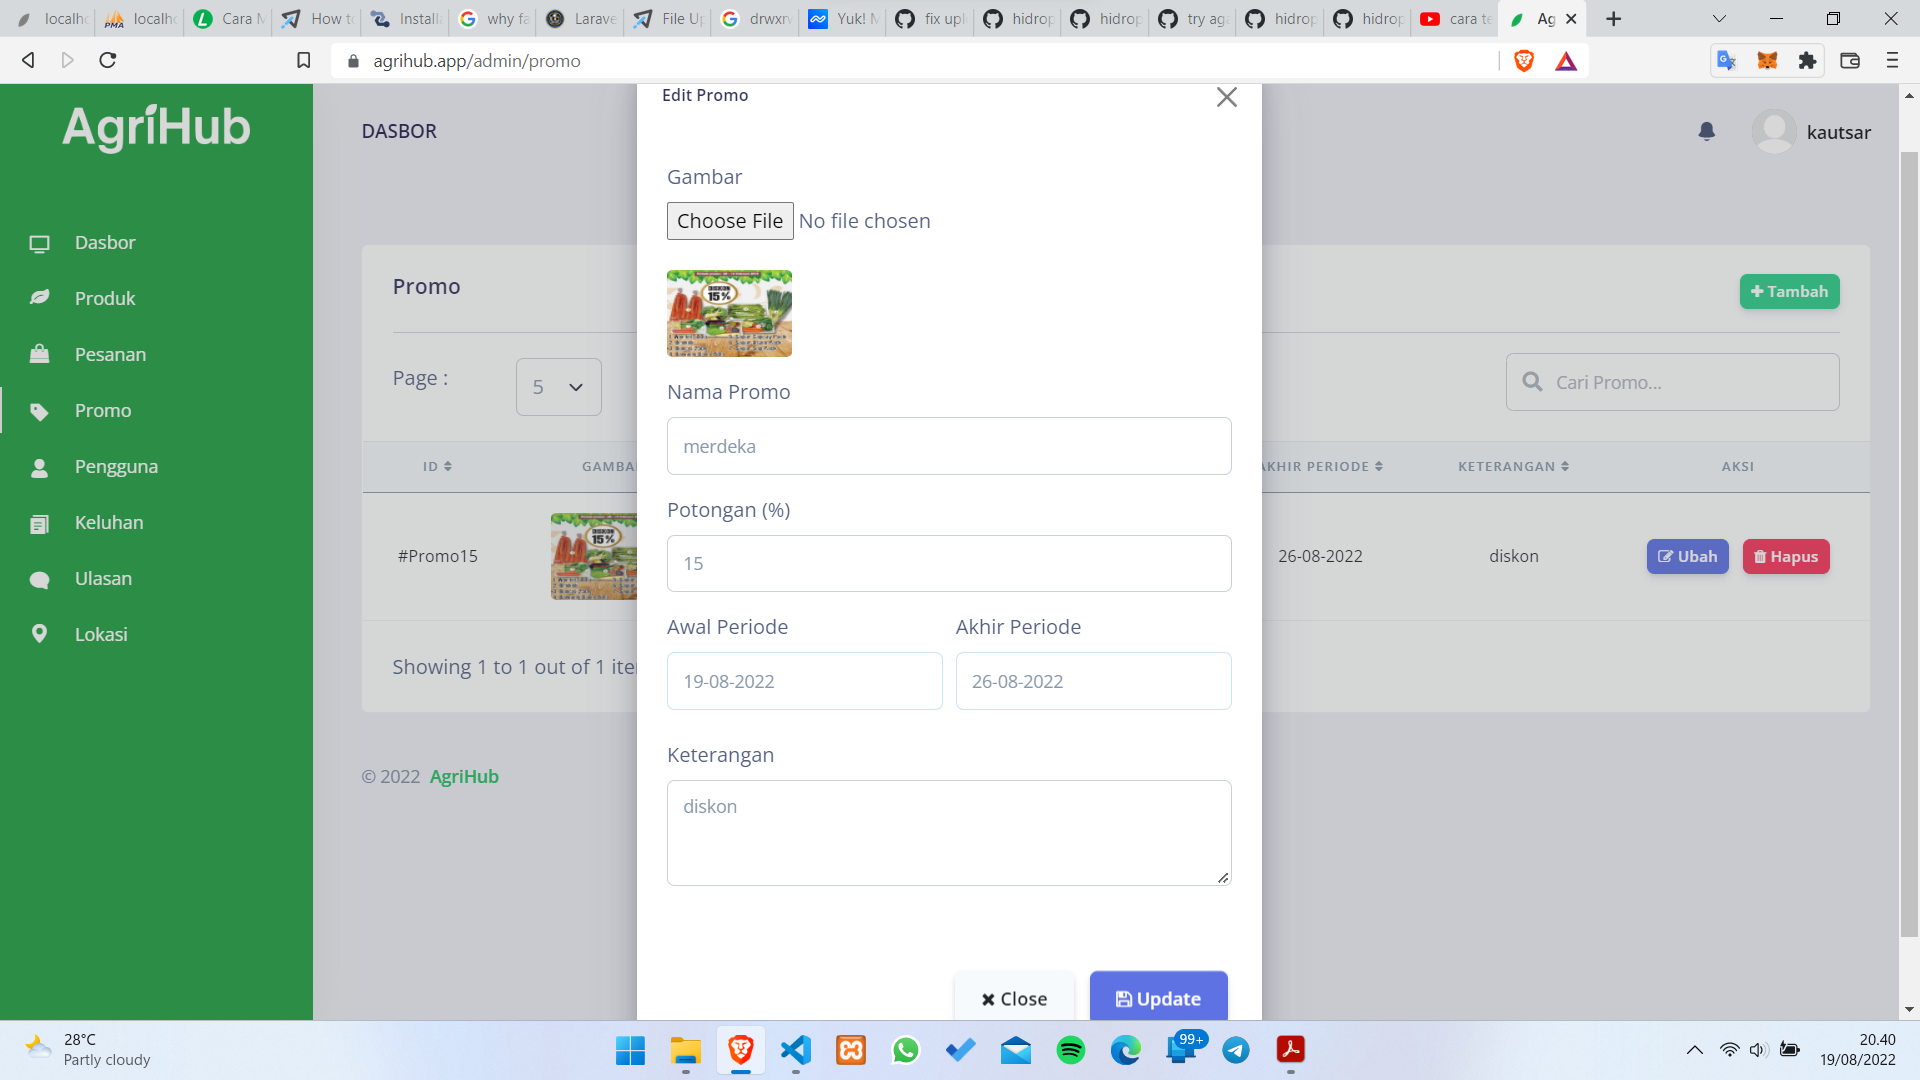
\includegraphics [width = 14.3cm, height= 9cm]{gambar/admin/ubah_promo}}
				\caption{Halaman Ubah Promo}
				\label{ubah_promo}
			\end{figure}

			\par Pada halaman pengguna ini admin data melihat semua data pengguna yang sudah terdaftar diaplikasi AgriHub ini baik itu admin, penjual maupun pembeli, serta dapat memblokir penjual atau pembeli yang melanggar. Juga dapat menambahkan penjual baru disini.

			\begin{figure}[H]
				\centering
				{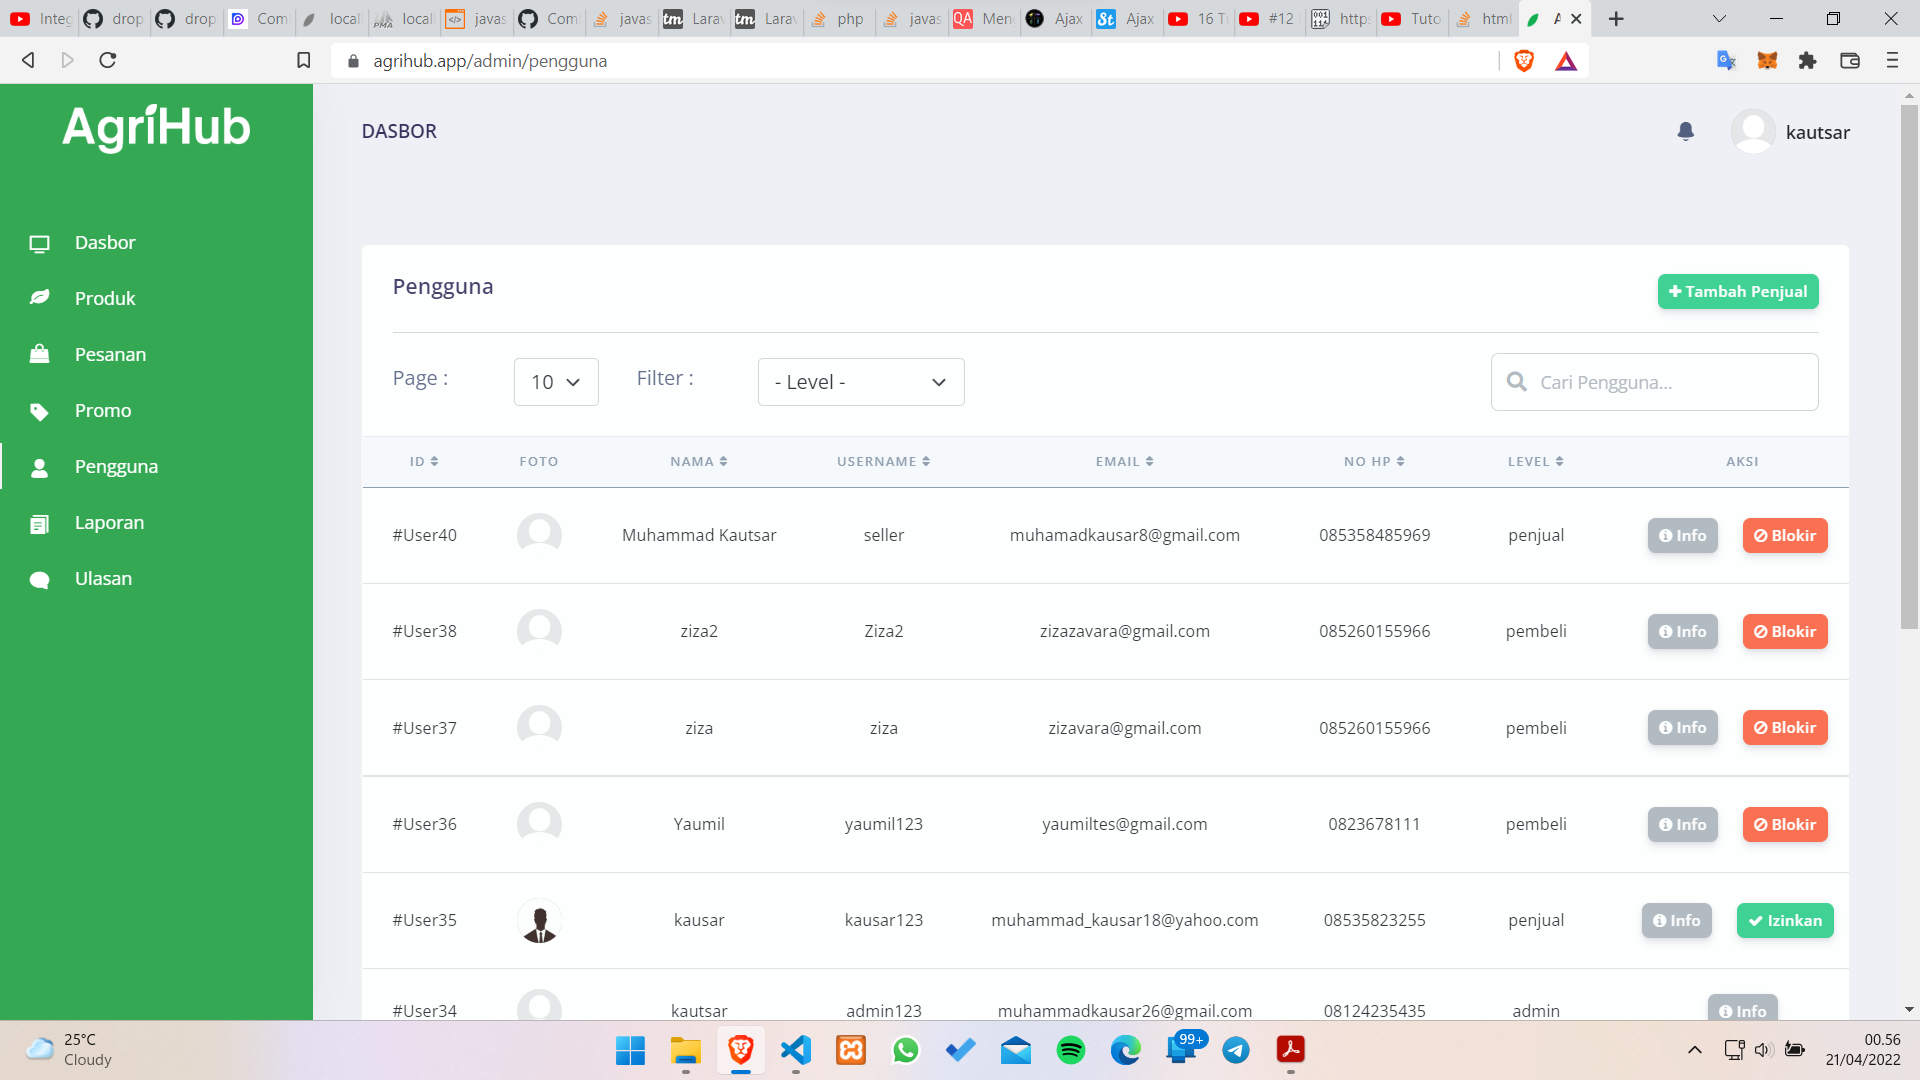
\includegraphics [width = 14.3cm, height= 9cm]{gambar/admin/pengguna}}
				\caption{Halaman Pengguna}
				\label{pengguna}
			\end{figure}

			\begin{figure}[H]
				\centering
				{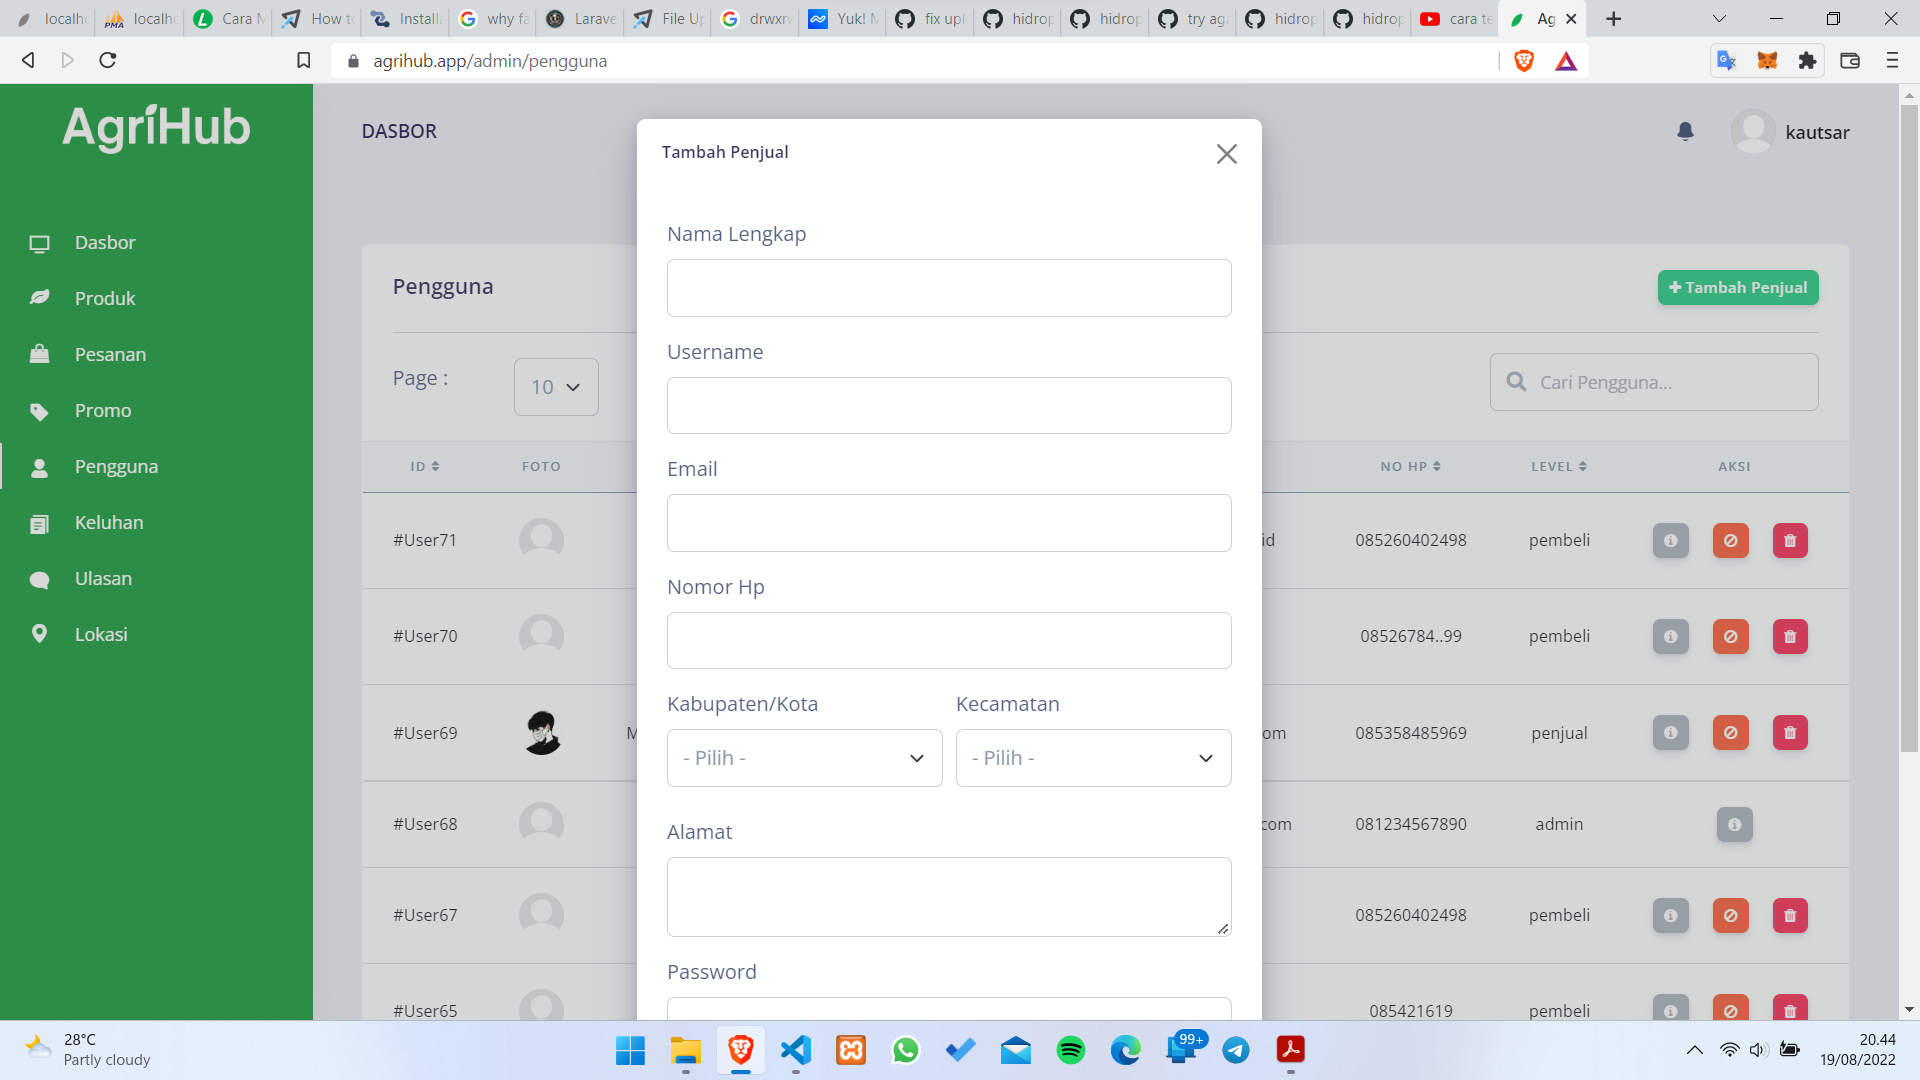
\includegraphics [width = 14.3cm, height= 9cm]{gambar/admin/tambah_pengguna}}
				\caption{Halaman Tambah Pengguna}
				\label{tambah_pengguna}
			\end{figure}

			\begin{figure}[H]
				\centering
				{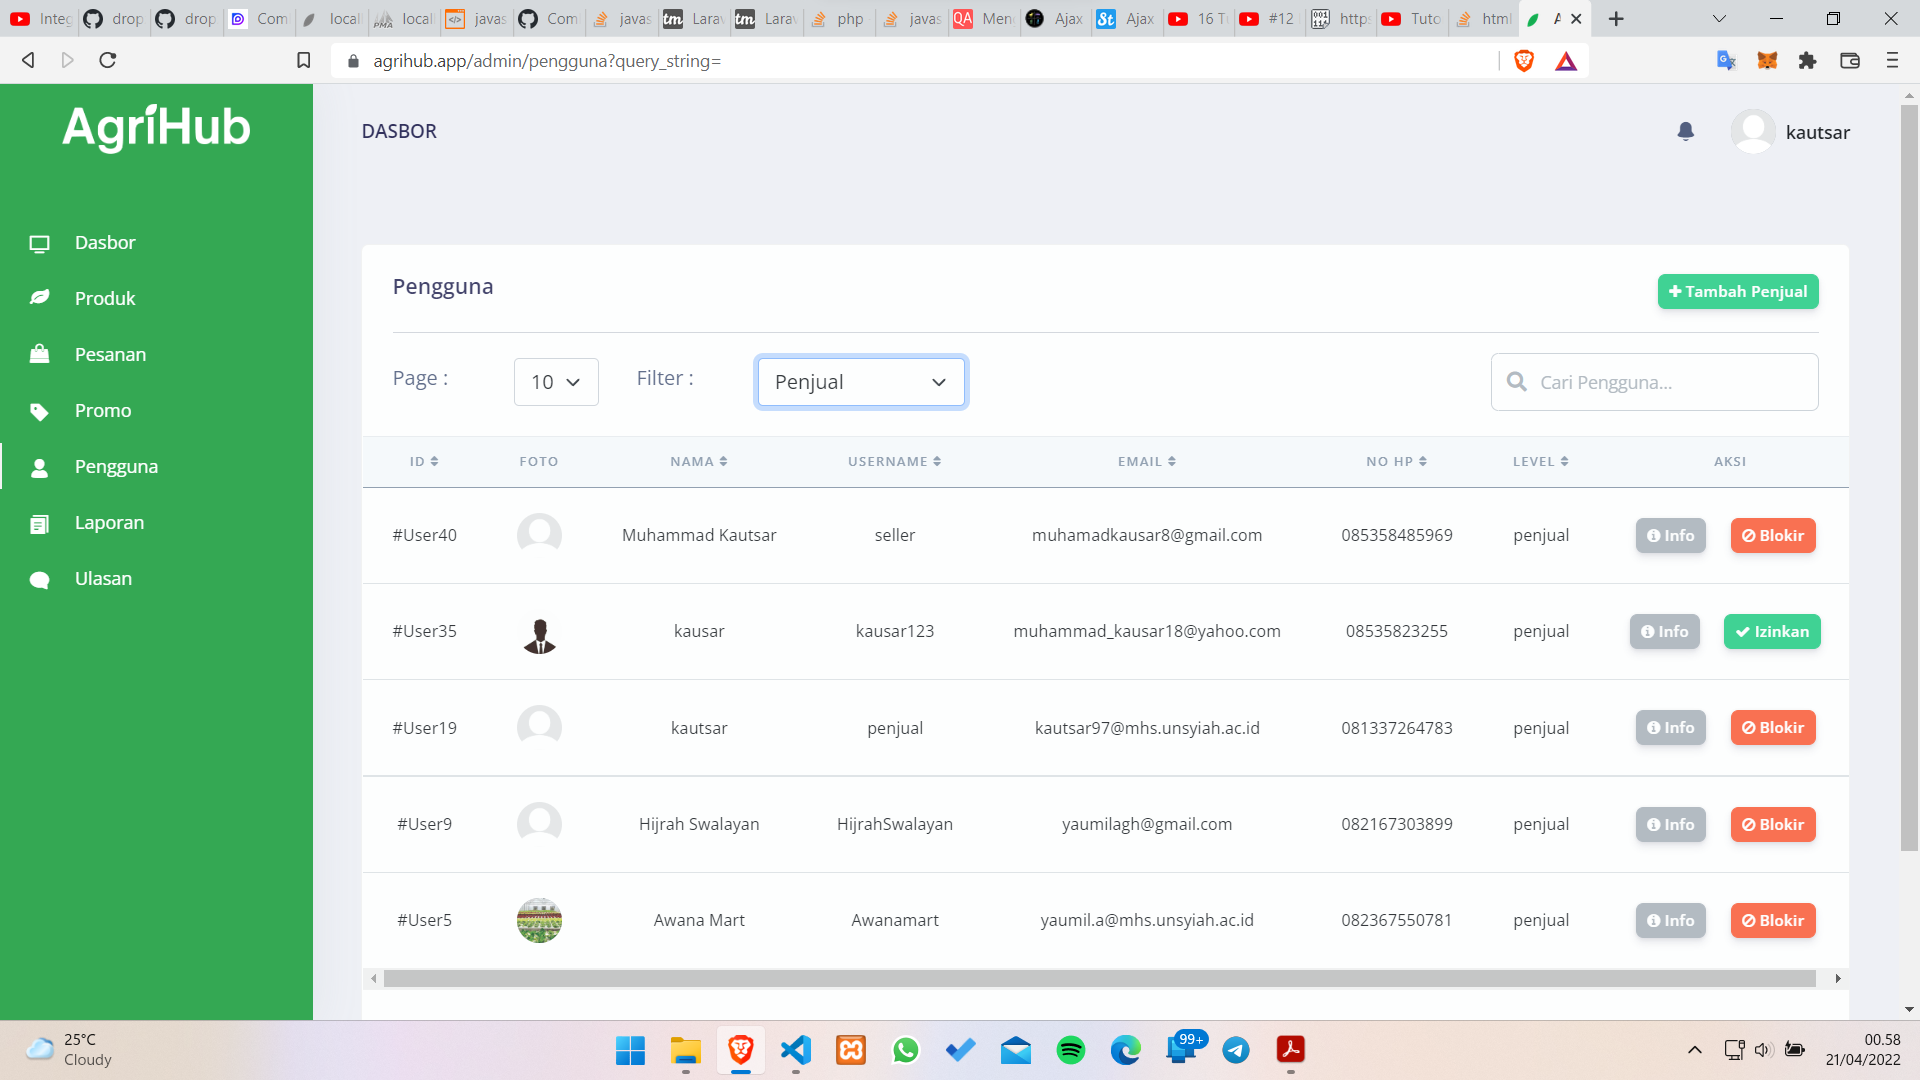
\includegraphics [width = 14.3cm, height= 9cm]{gambar/admin/filter_pengguna}}
				\caption{Halaman Filter Pengguna}
				\label{filter_pengguna}
			\end{figure}

			\par Pada halaman laporan ini admin dapat melihat laporan-laporan yang masuk dari para pembeli terhadap penjual.

			\begin{figure}[H]
				\centering
				{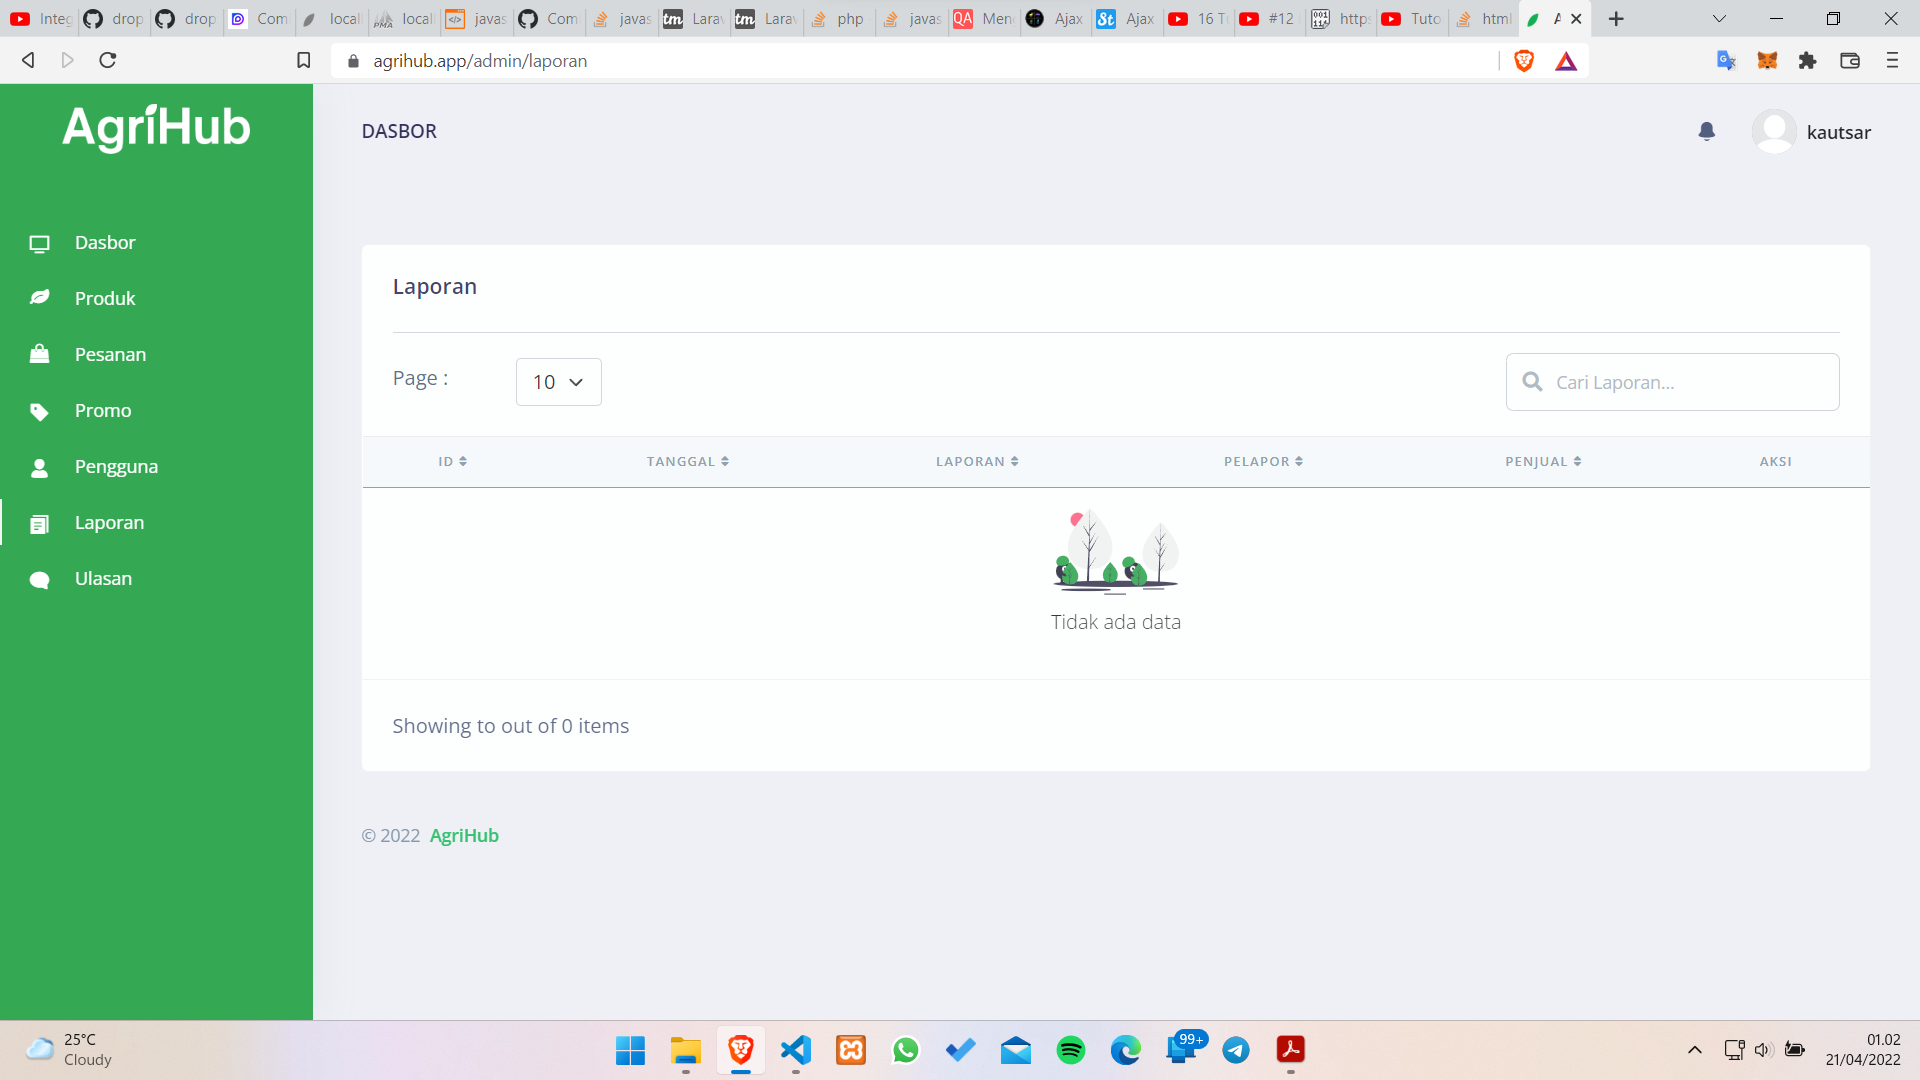
\includegraphics [width = 14.3cm, height= 9cm]{gambar/admin/laporan}}
				\caption{Halaman Laporan}
				\label{laporan}
			\end{figure}

			\par Admin juga dapat melihat semua ulasan dari para pembeli terhadap produk yang ditawarkan penjual melalui halaman ulasan ini.

			\begin{figure}[H]
				\centering
				{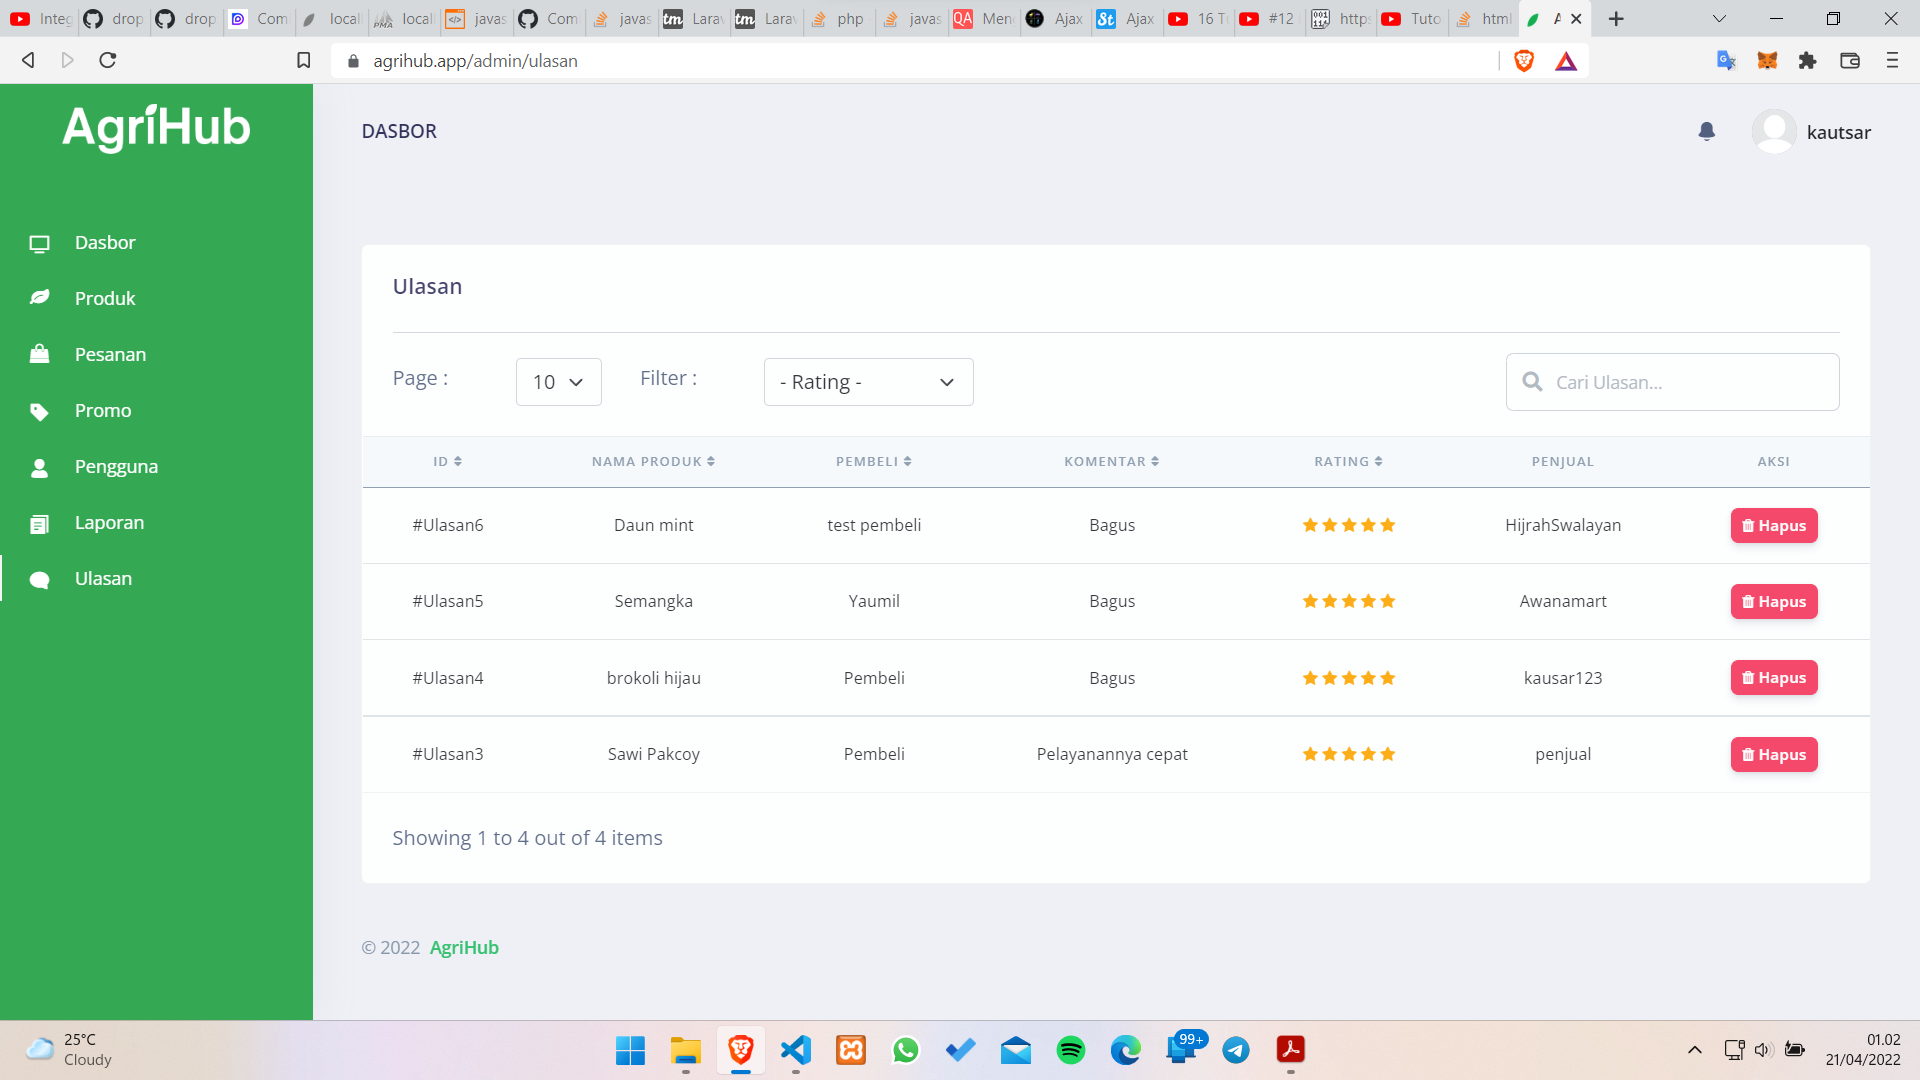
\includegraphics [width = 14.3cm, height= 9cm]{gambar/admin/ulasan_admin}}
				\caption{Halaman Ulasan Admin}
				\label{ulasan_admin}
			\end{figure}

			\begin{figure}[H]
				\centering
				{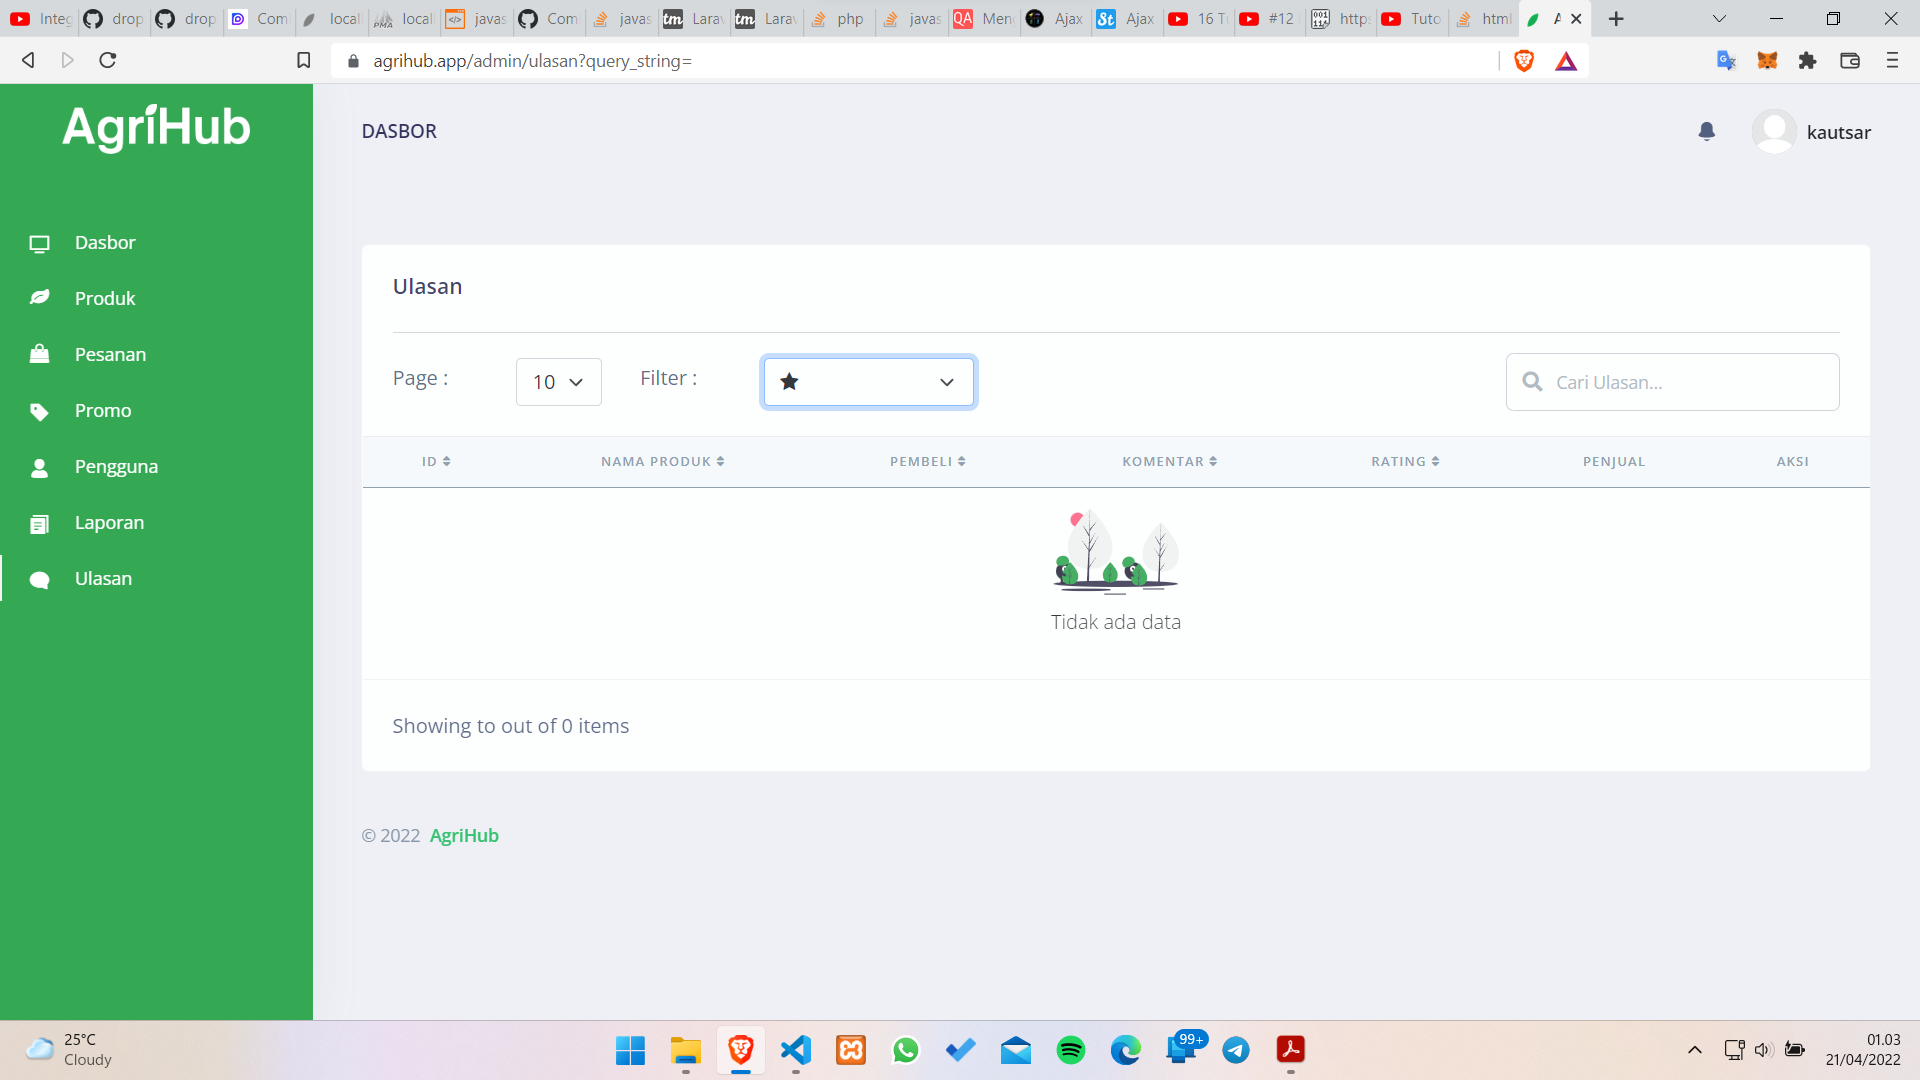
\includegraphics [width = 14.3cm, height= 9cm]{gambar/admin/filter_ulasan}}
				\caption{Halaman Filter Ulasan Admin}
				\label{filter_ulasan}
			\end{figure}

			\item Antarmuka Aplikasi Bagian Penjual
			\par Antarmuka pada bagian penjual pada dasarnya hampir sama seperti antarmuka pada bagian admin hanya saja beberapa menunya saja yang berbeda. Ketika pertama kali mengakses aplikasi, maka
			akan ditampilkan halaman home kemudian apabila si penjual ingin masuk kedalam aplikasi dapat menklik tombol masuk yang ada dipojok kanan atas lalu mengisi email dan password yang sudah terdaftar.

			\begin{figure}[H]
				\centering
				{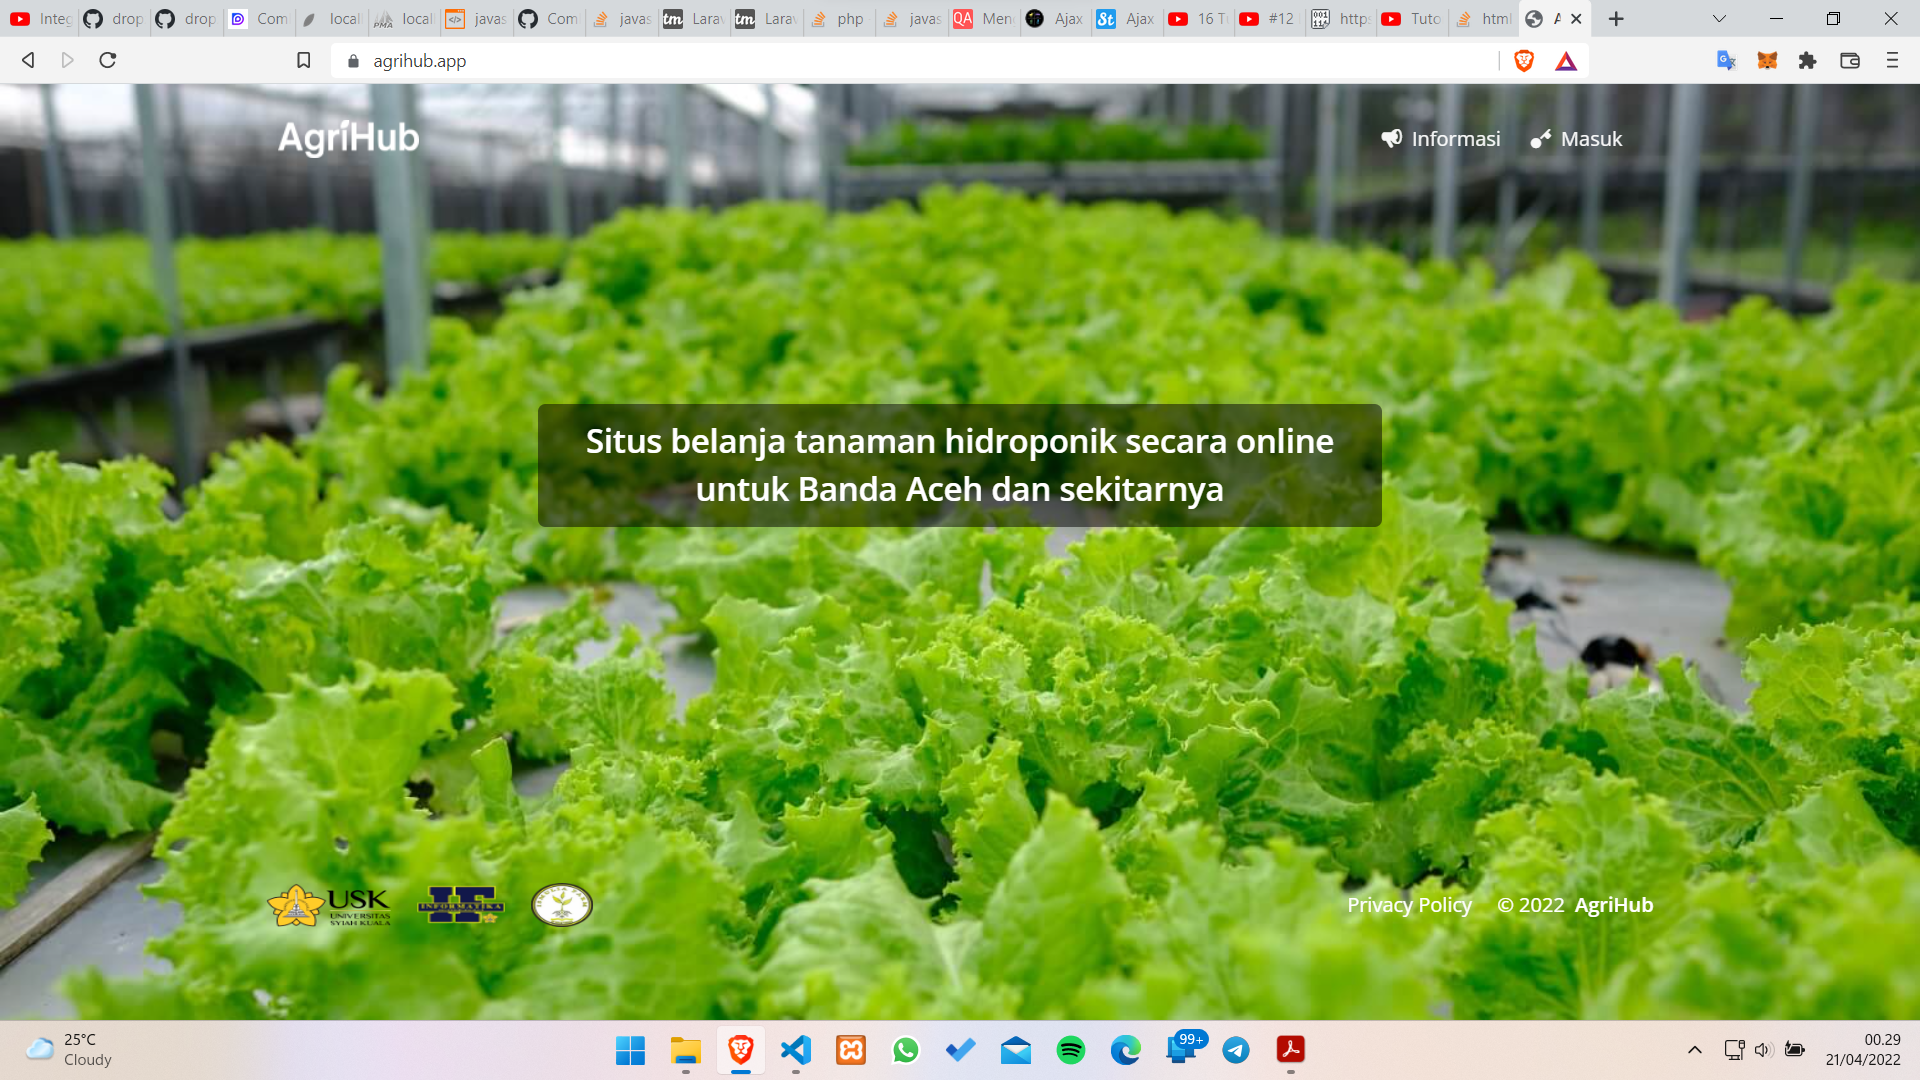
\includegraphics [width = 14.3cm, height= 9cm]{gambar/homepage}}
				\caption{Halaman Home}
				\label{homepage}
			\end{figure}

			\begin{figure}[H]
				\centering
				{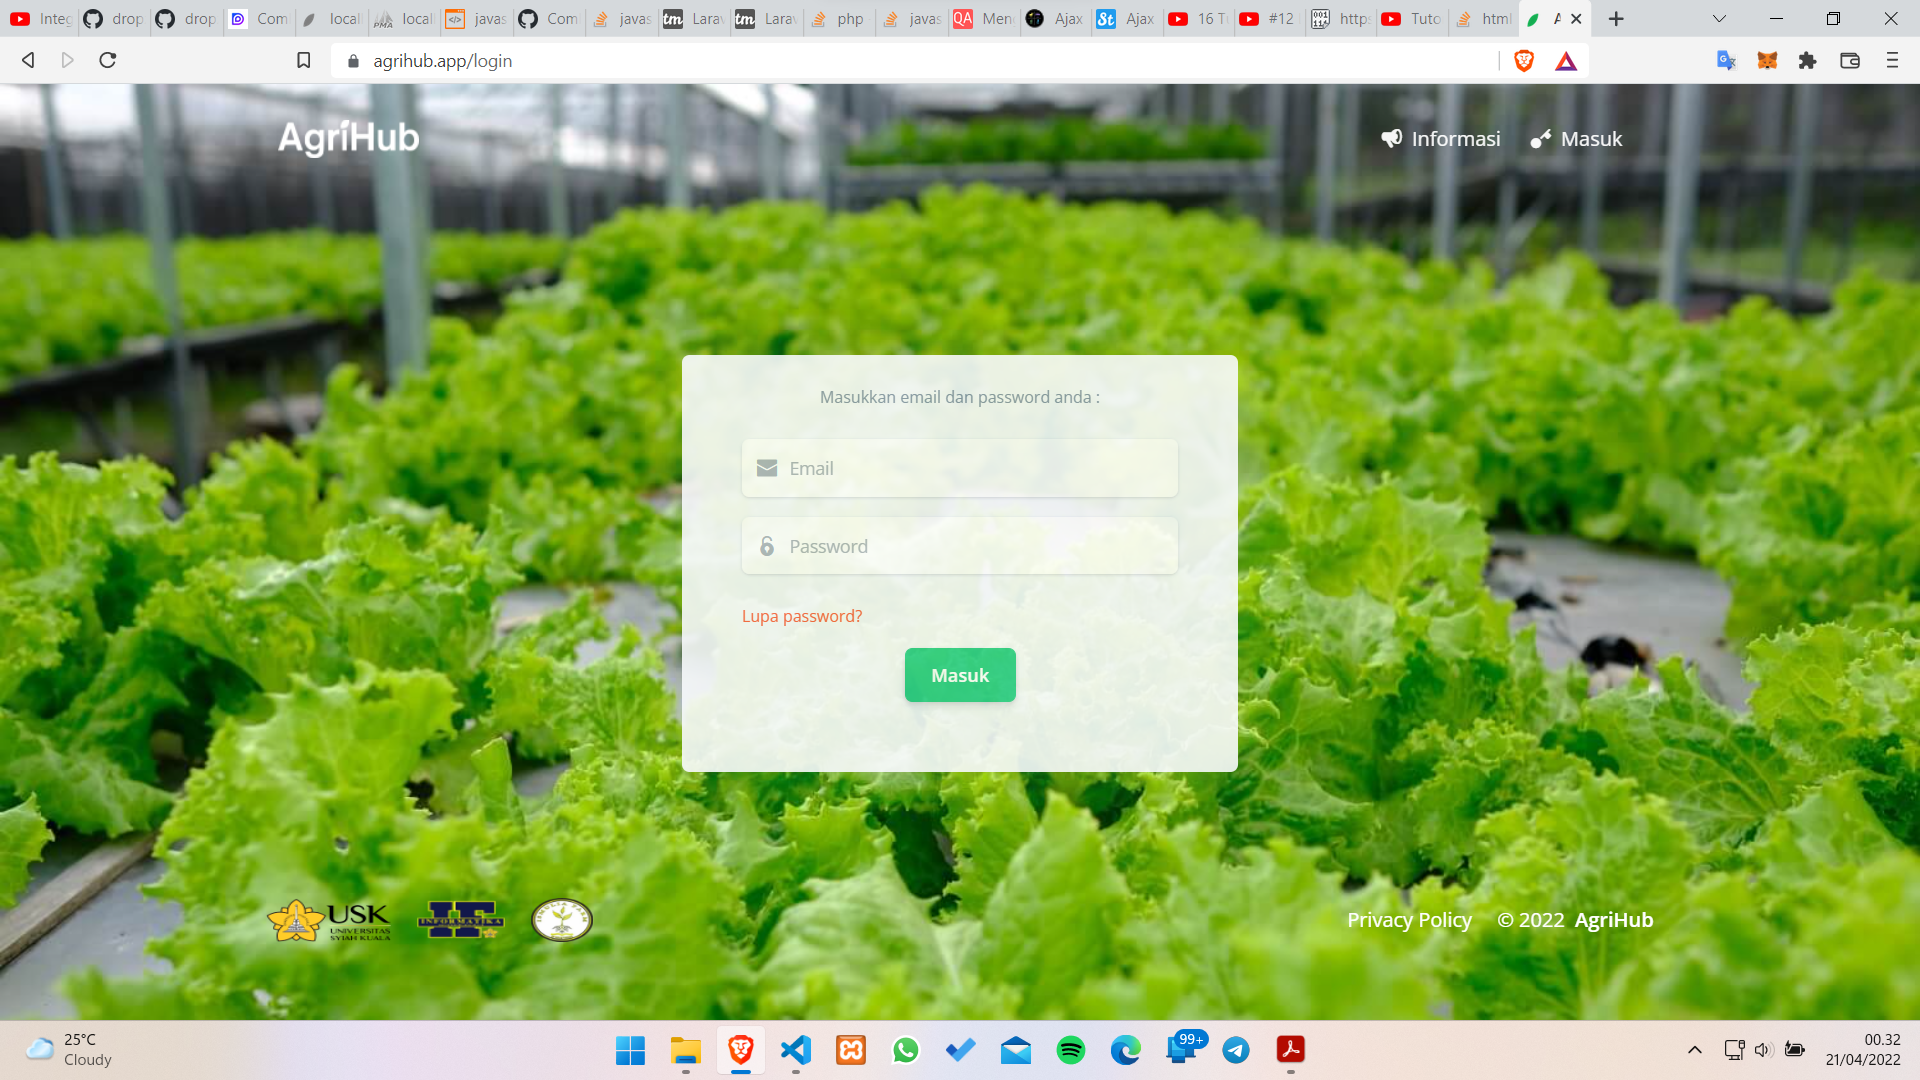
\includegraphics [width = 14.3cm, height= 9cm]{gambar/login}}
				\caption{Halaman Login}
				\label{login}
			\end{figure}

			\par Apabila penjual belum terdaftar diaplikasi dapat menklik tombol informasi yang ada disamping tombol masuk untuk mengetahui tata cara mendaftar sebagai penjual diaplikasi AgriHub ini.

			\begin{figure}[H]
				\centering
				{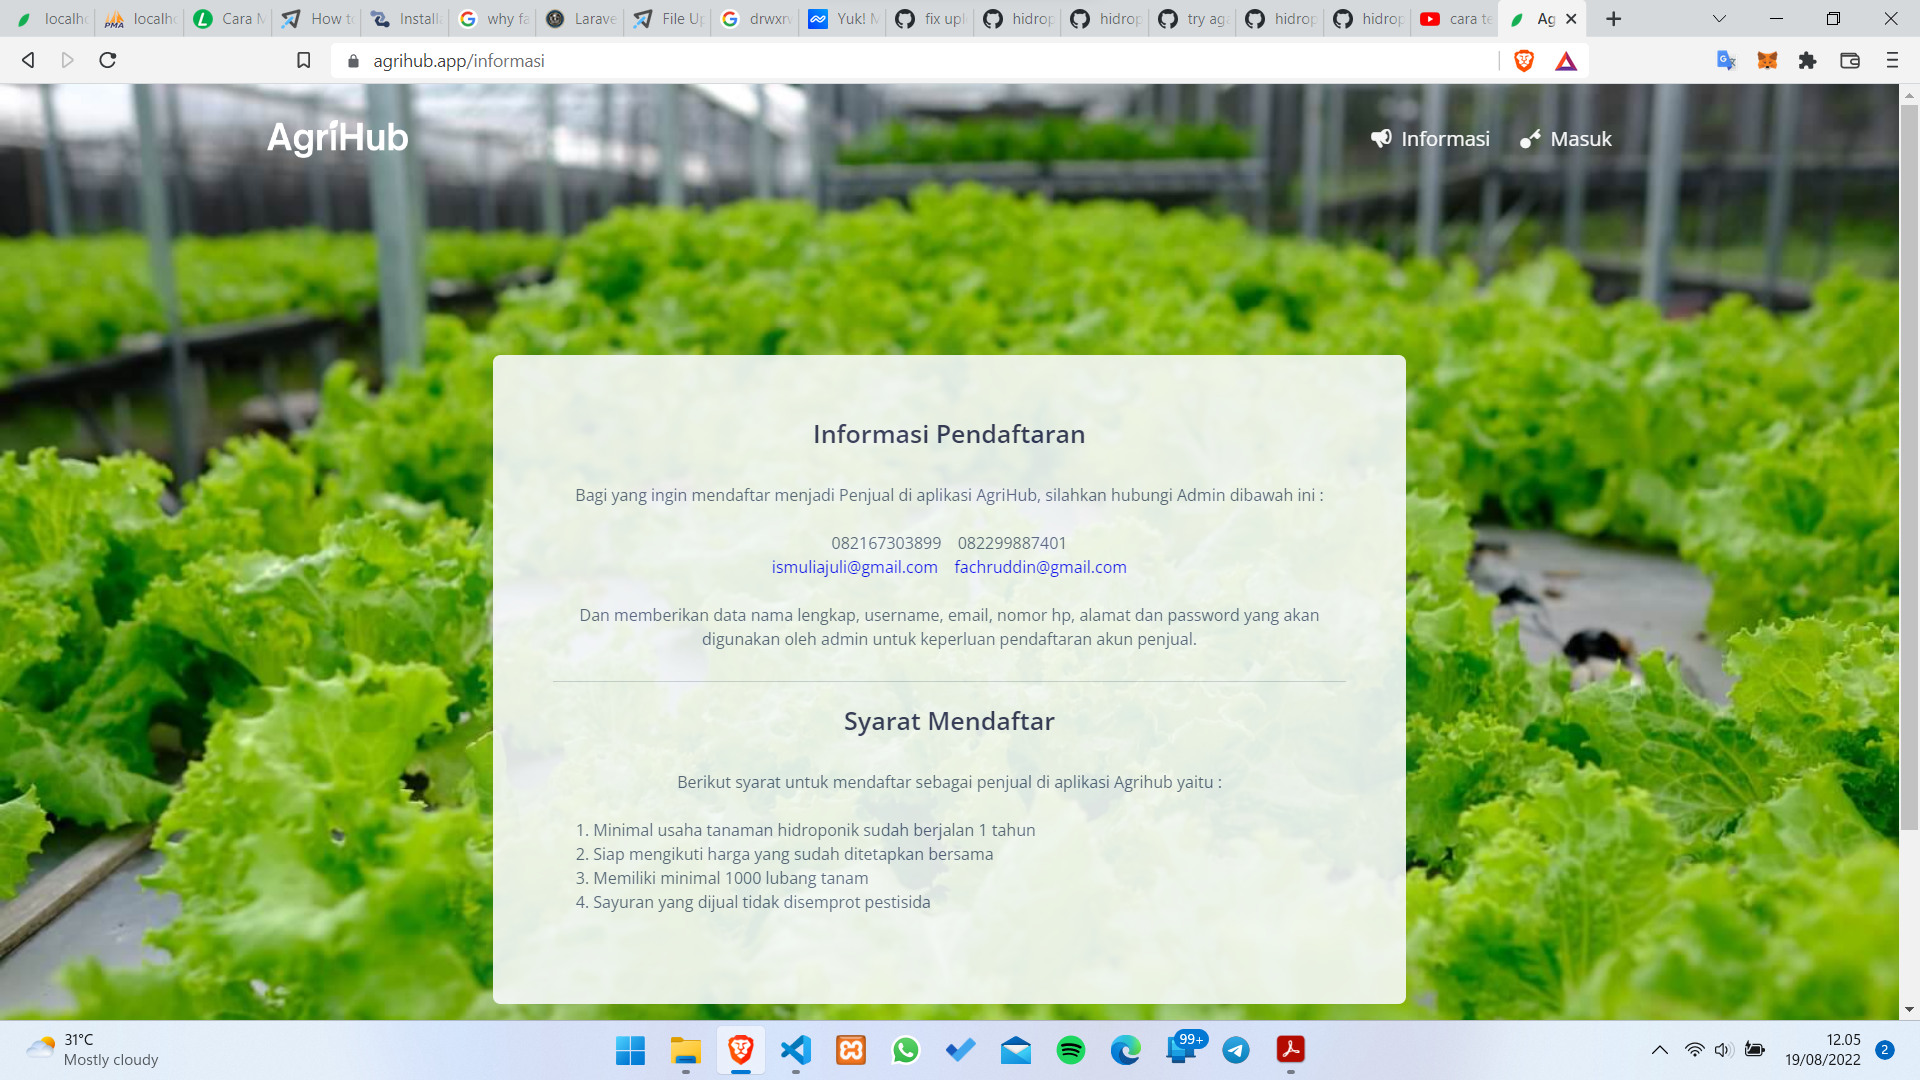
\includegraphics [width = 14.3cm, height= 9cm]{gambar/informasi}}
				\caption{Halaman Informasi}
				\label{informasi}
			\end{figure}

			\par Apabila penjual sudah terdaftar tapi tidak bisa masuk kedalam aplikasi bisa jadi akunnya penjual lagi diblokir oleh admin karna melakukan kesalahan. Supaya akunnya penjual dapat digunakan kembali bisa menghubungi admin terlebih dahulu.

			\begin{figure}[H]
				\centering
				{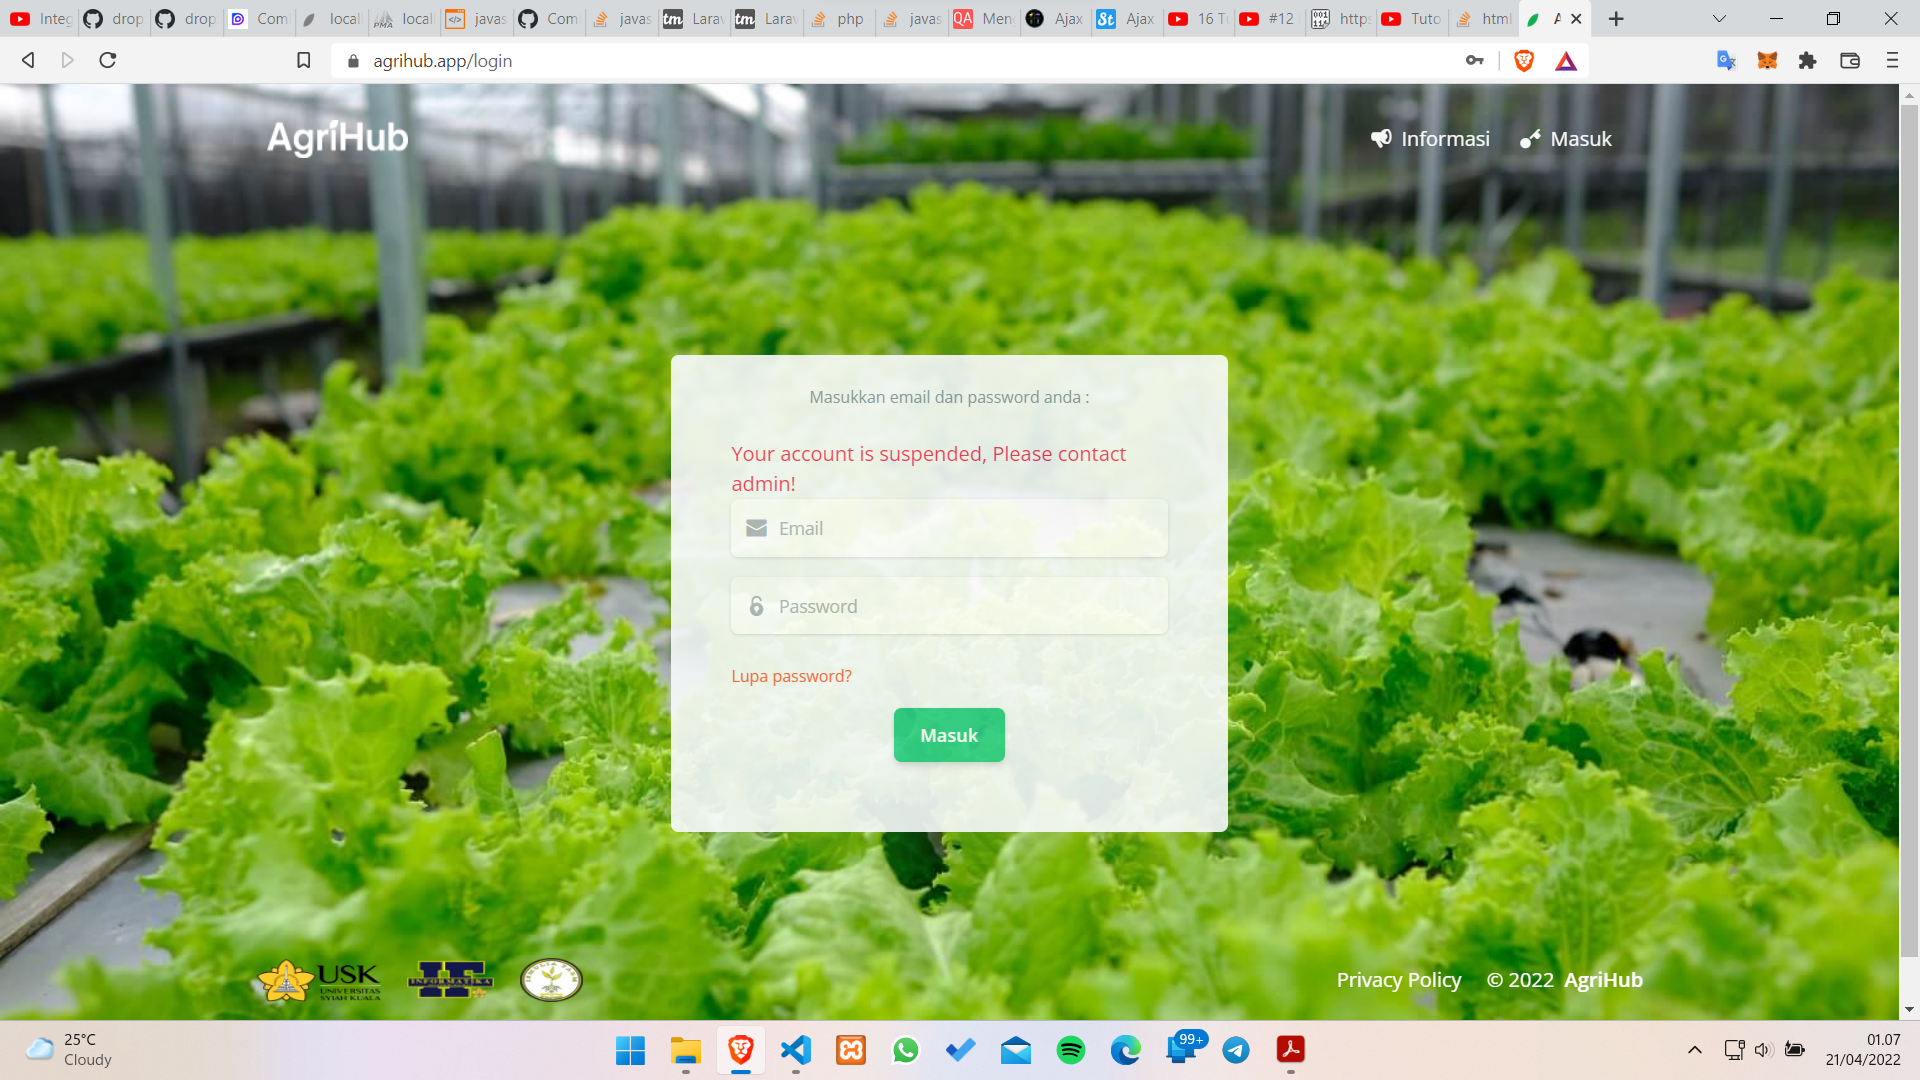
\includegraphics [width = 14.3cm, height= 9cm]{gambar/diblokir}}
				\caption{Halaman Diblokir}
				\label{diblokir}
			\end{figure}

			\par Dan apabila si penjual lupa password akunnya dapat menklik tombol lupa password yang ada dihalaman login kemudian mengisikan emailnya, supaya nanti dikirimkan email reset password ke alamat email terdaftar untuk mengubah passwordnya.

			\begin{figure}[H]
				\centering
				{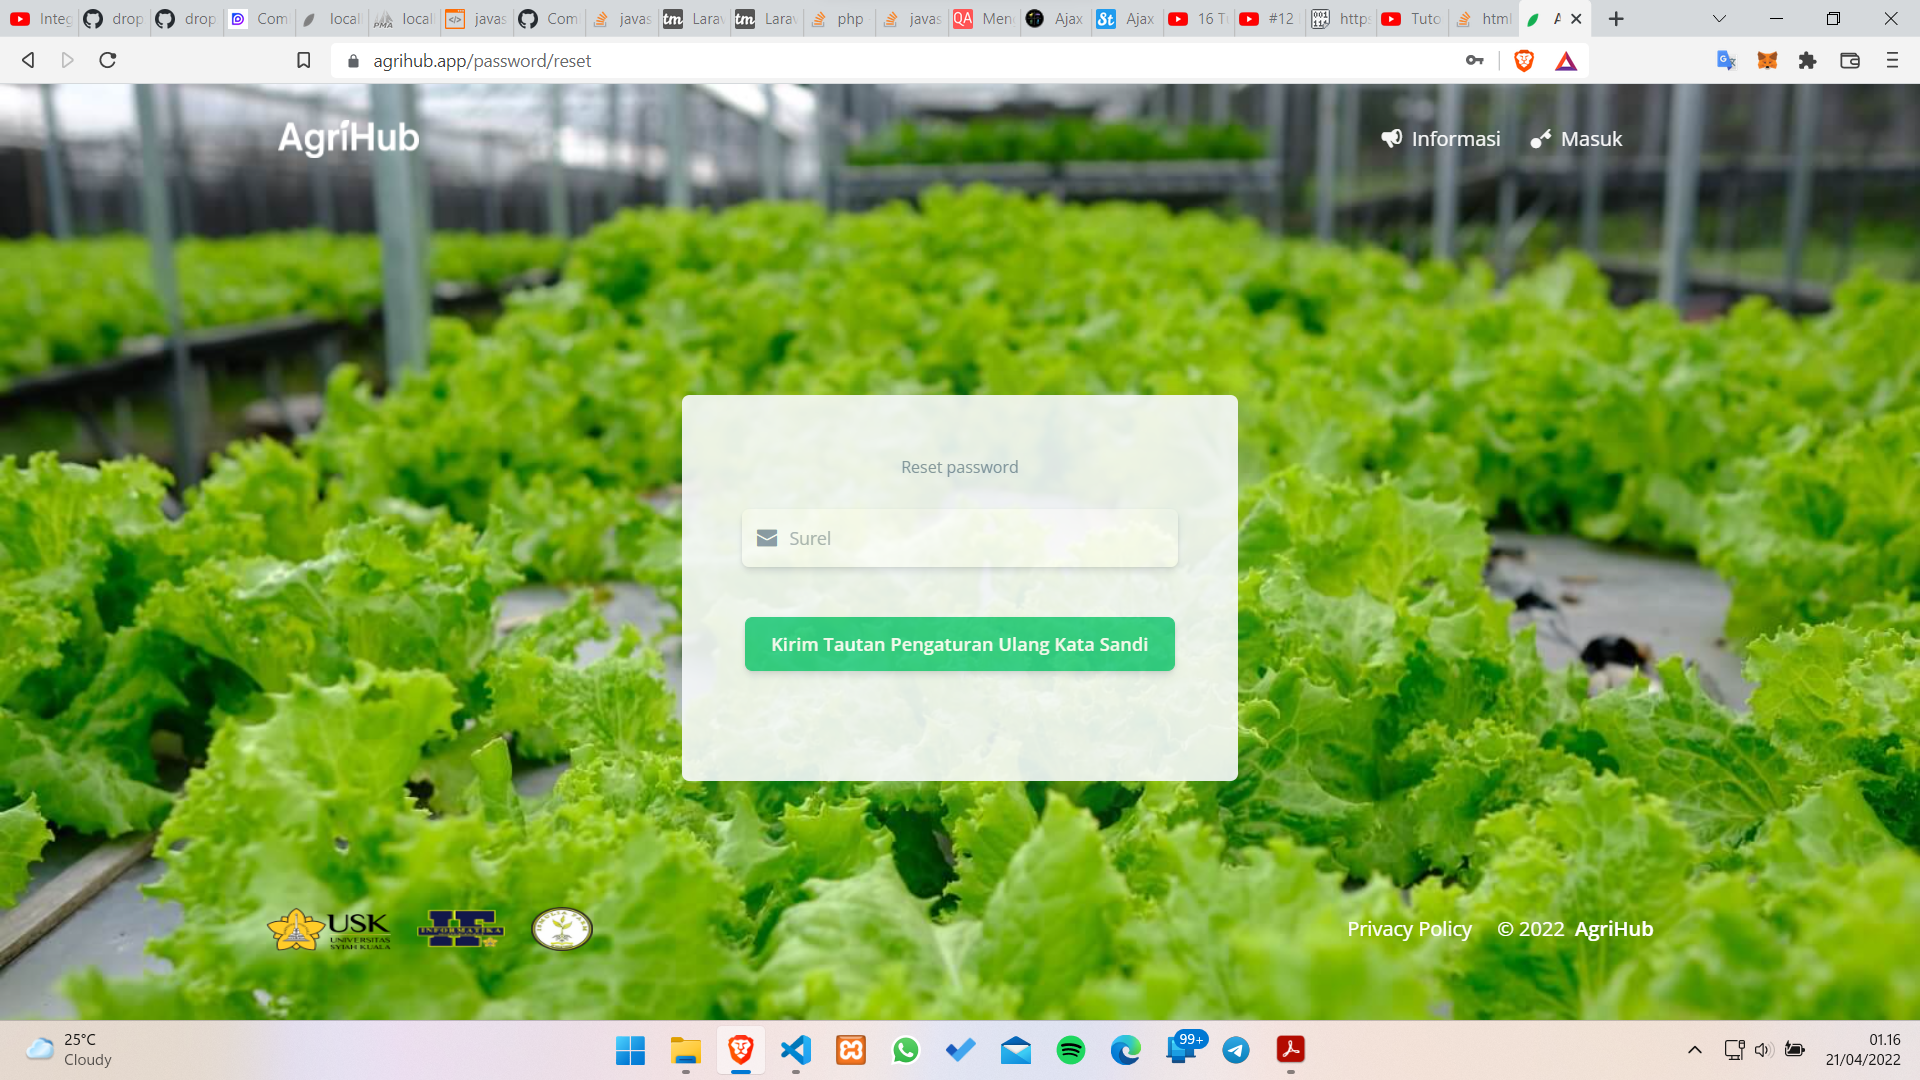
\includegraphics [width = 14.3cm, height= 9cm]{gambar/lupa_password}}
				\caption{Halaman Lupa Password}
				\label{lupa_password}
			\end{figure}

			\par Setelah penjual melakukan login kedalam aplikasi, maka akan tampil halaman dashboard yang berisi keterangan mengenai jumlah order baru yang masuk, lagi diproses, dikirim, yang sudah selesai dan jumlah order yang batal, serta jumlah ulasan yang sudah diberikan oleh pembeli. Juga ada grafik jumlah pendapatan perbulan yang sudah diperoleh oleh penjual beserta dengan jumlah pesanan yang selesai dan batal perbulannya selama 6 bulan terakhir.

			\begin{figure}[H]
				\centering
				{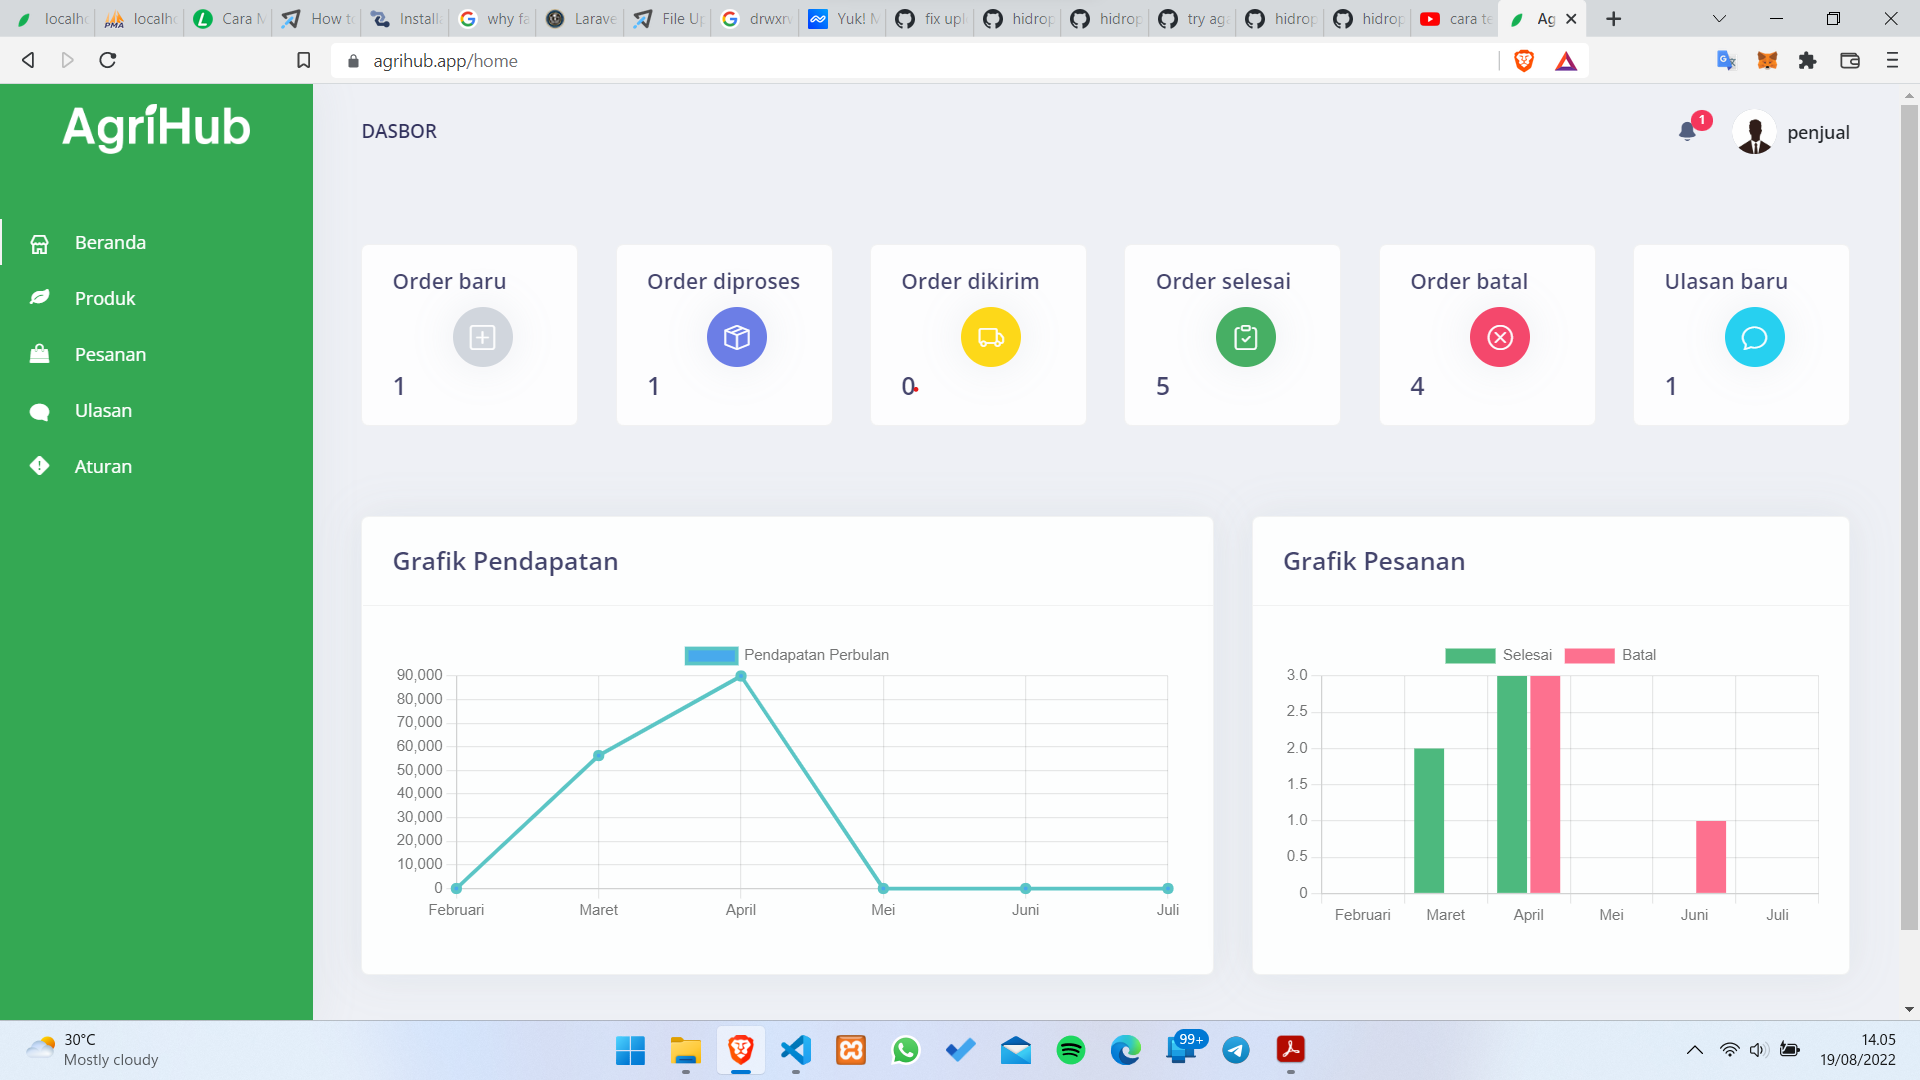
\includegraphics [width = 14.3cm, height= 9cm]{gambar/penjual/dashboard_penjual}}
				\caption{Halaman Dashboard Penjual}
				\label{dashboard_penjual}
			\end{figure}

			\par Pada halaman produk ini penjual dapat mengelola produknya yang ingin dijual seperti menambahkan produk baru, mengubah data produk yang sudah ada dan menghapus produk yang tidak ingin dijual lagi.

			\begin{figure}[H]
				\centering
				{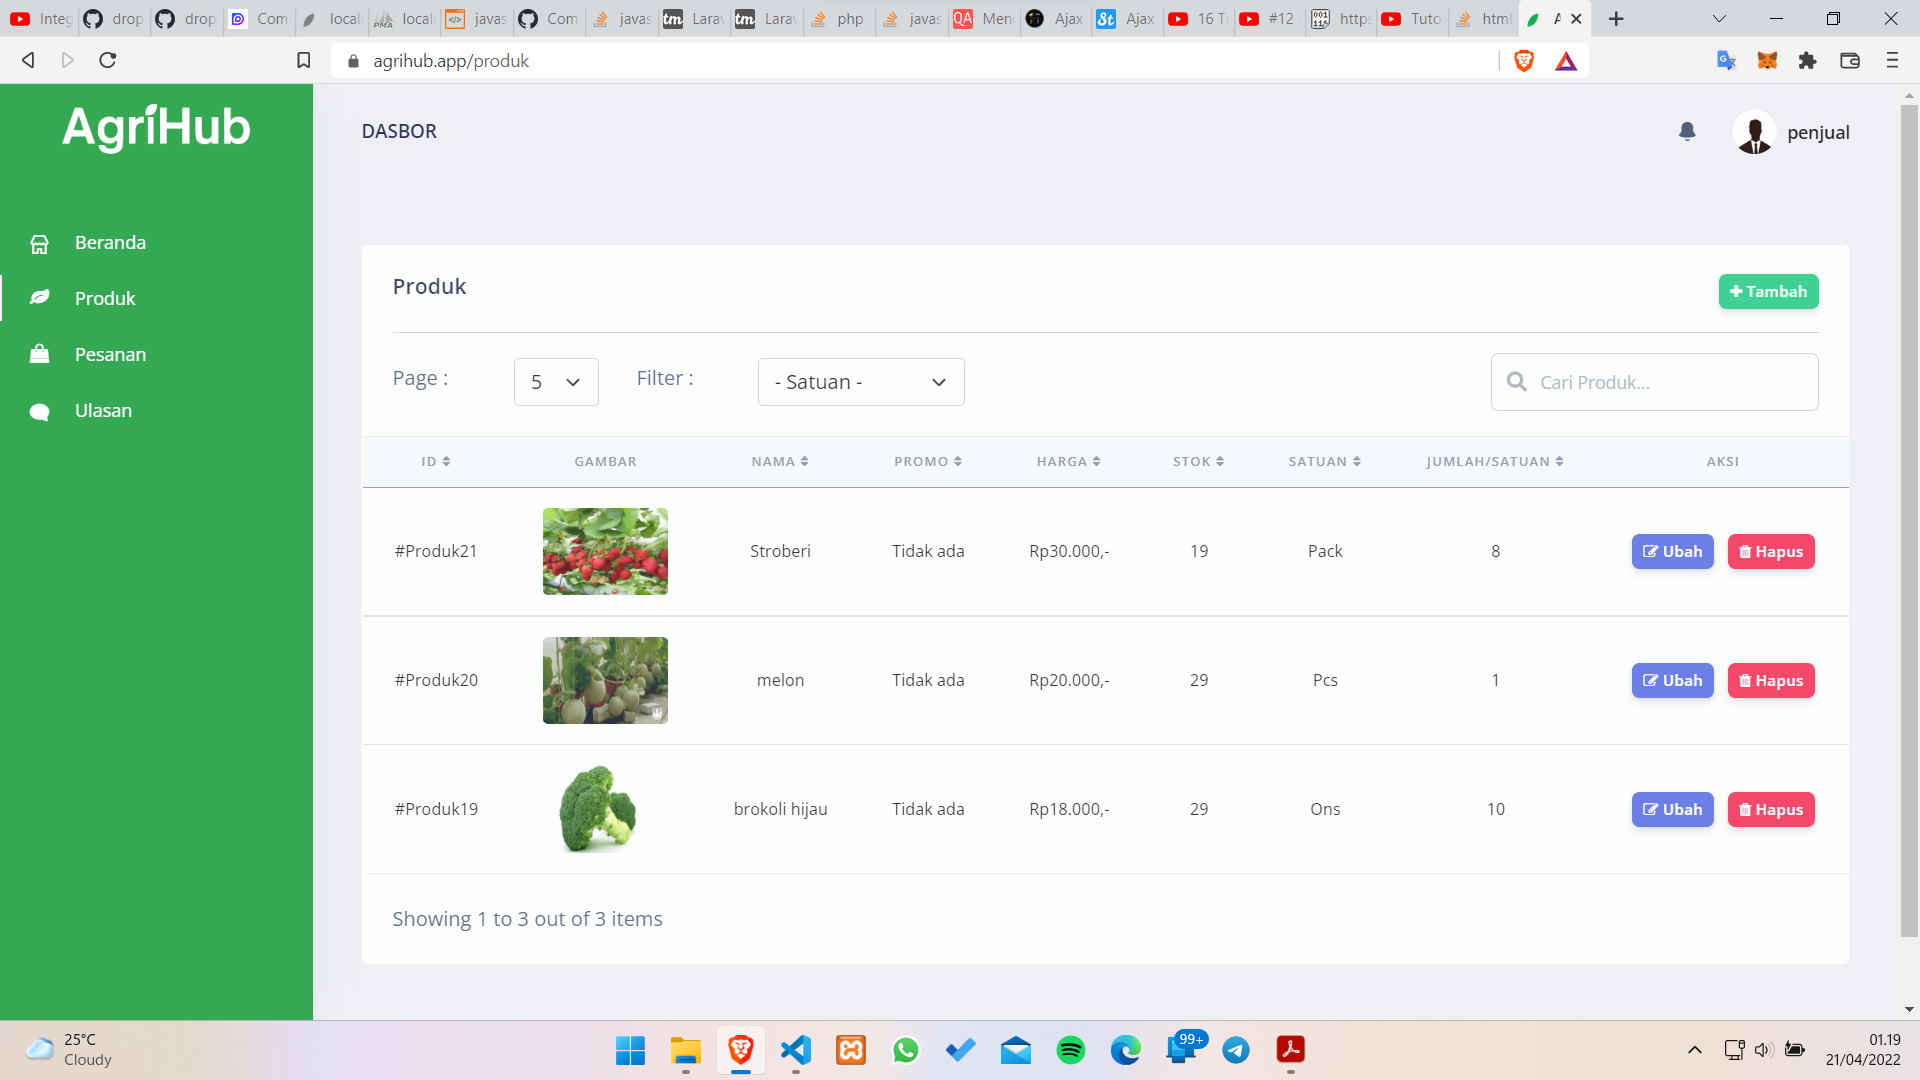
\includegraphics [width = 14.3cm, height= 9cm]{gambar/penjual/produk_penjual}}
				\caption{Halaman Produk Penjual}
				\label{produk_penjual}
			\end{figure}

			\par Pada form tambah produk ini penjual harus mengisi data-data produk seperti gambar, nama, harga, stok, satuan dan jumlah per satuan. Ada juga kolom promo disini penjual bisa memakai promo yang disediakan oleh admin jika berkenan dan ada kolom keterangan yang bersifat opsional untuk diisi.

			\begin{figure}[H]
				\centering
				{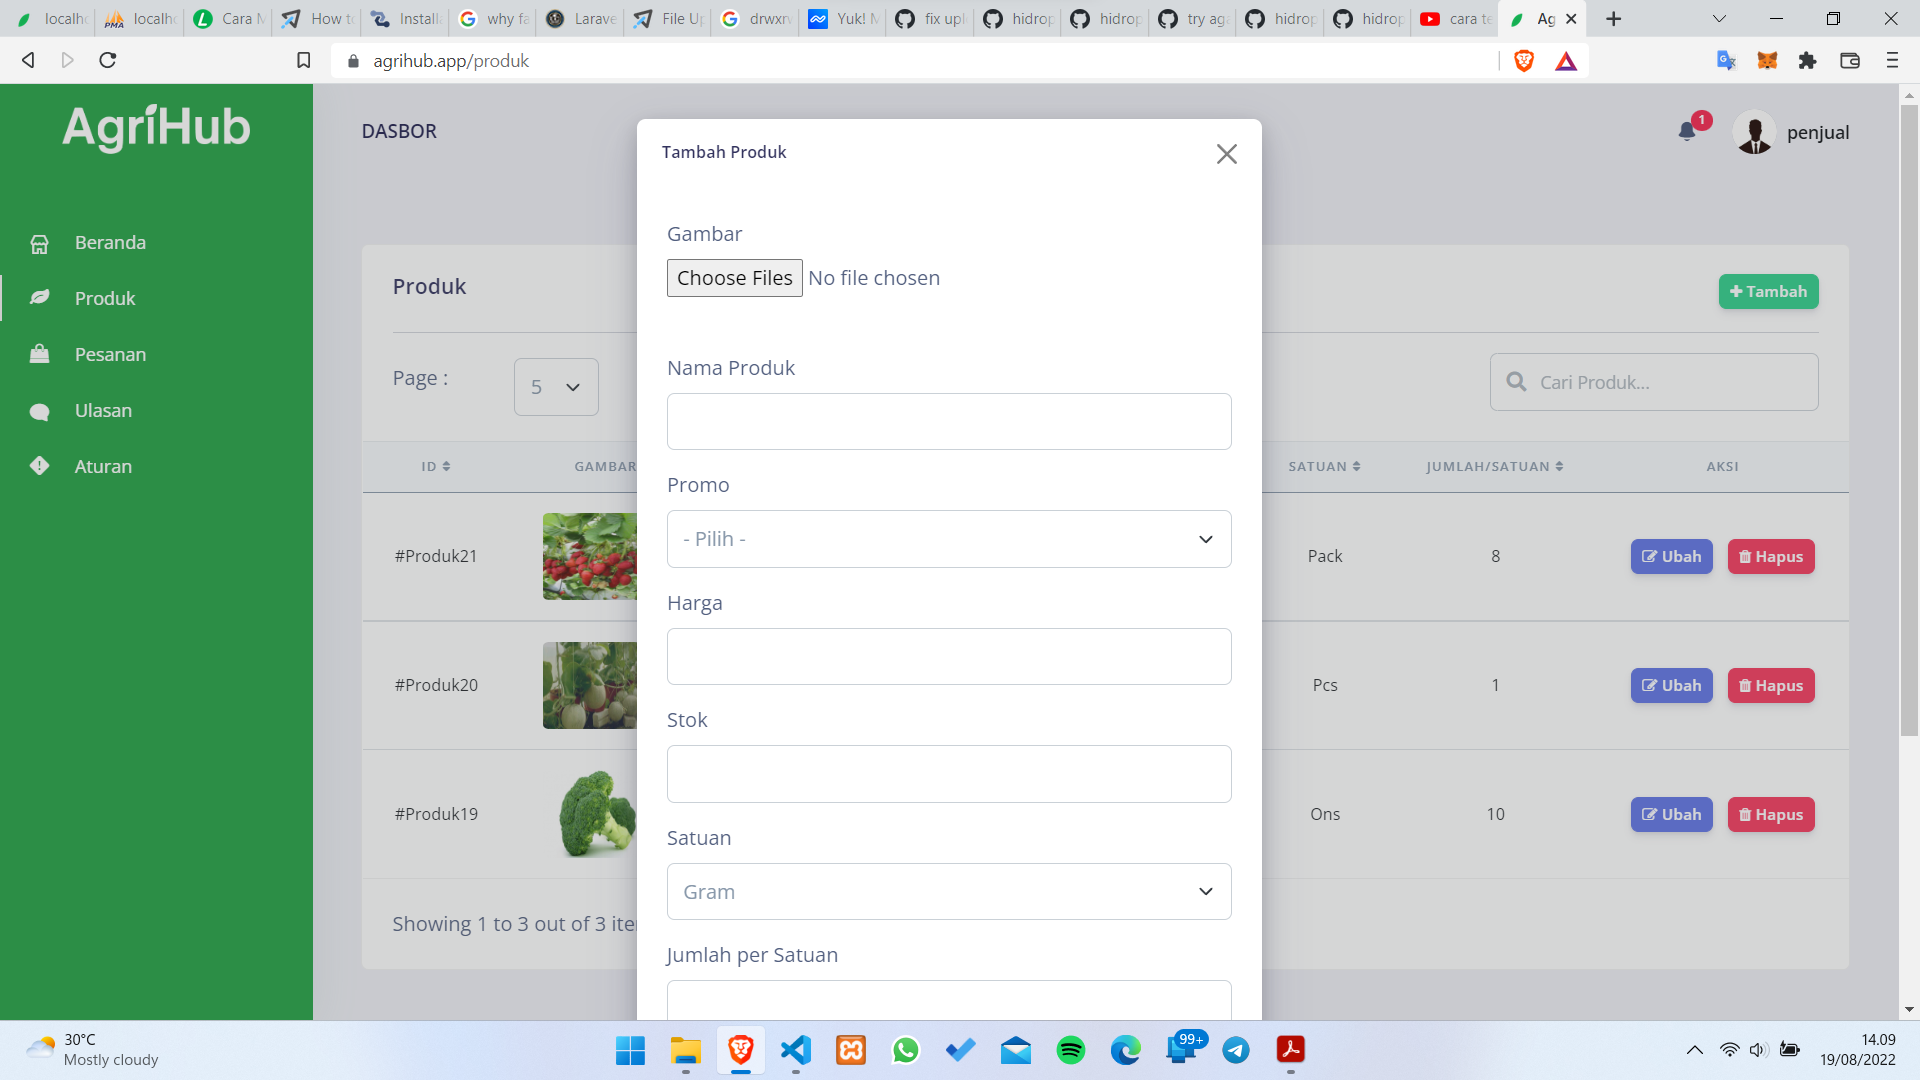
\includegraphics [width = 14.3cm, height= 9cm]{gambar/penjual/tambah_produk}}
				\caption{Halaman Tambah Produk}
				\label{tambah_produk}
			\end{figure}

			\par Penjual juga dapat mengubah detail produk yang ia jual melalui halaman ubah produk ini. Disini penjual dapat menambah atau menghapus gambar produk yang ia jual dan dapat mengubah detail produknya seperti nama, harga, stok, satuan dan lainnya.

			\begin{figure}[H]
				\centering
				{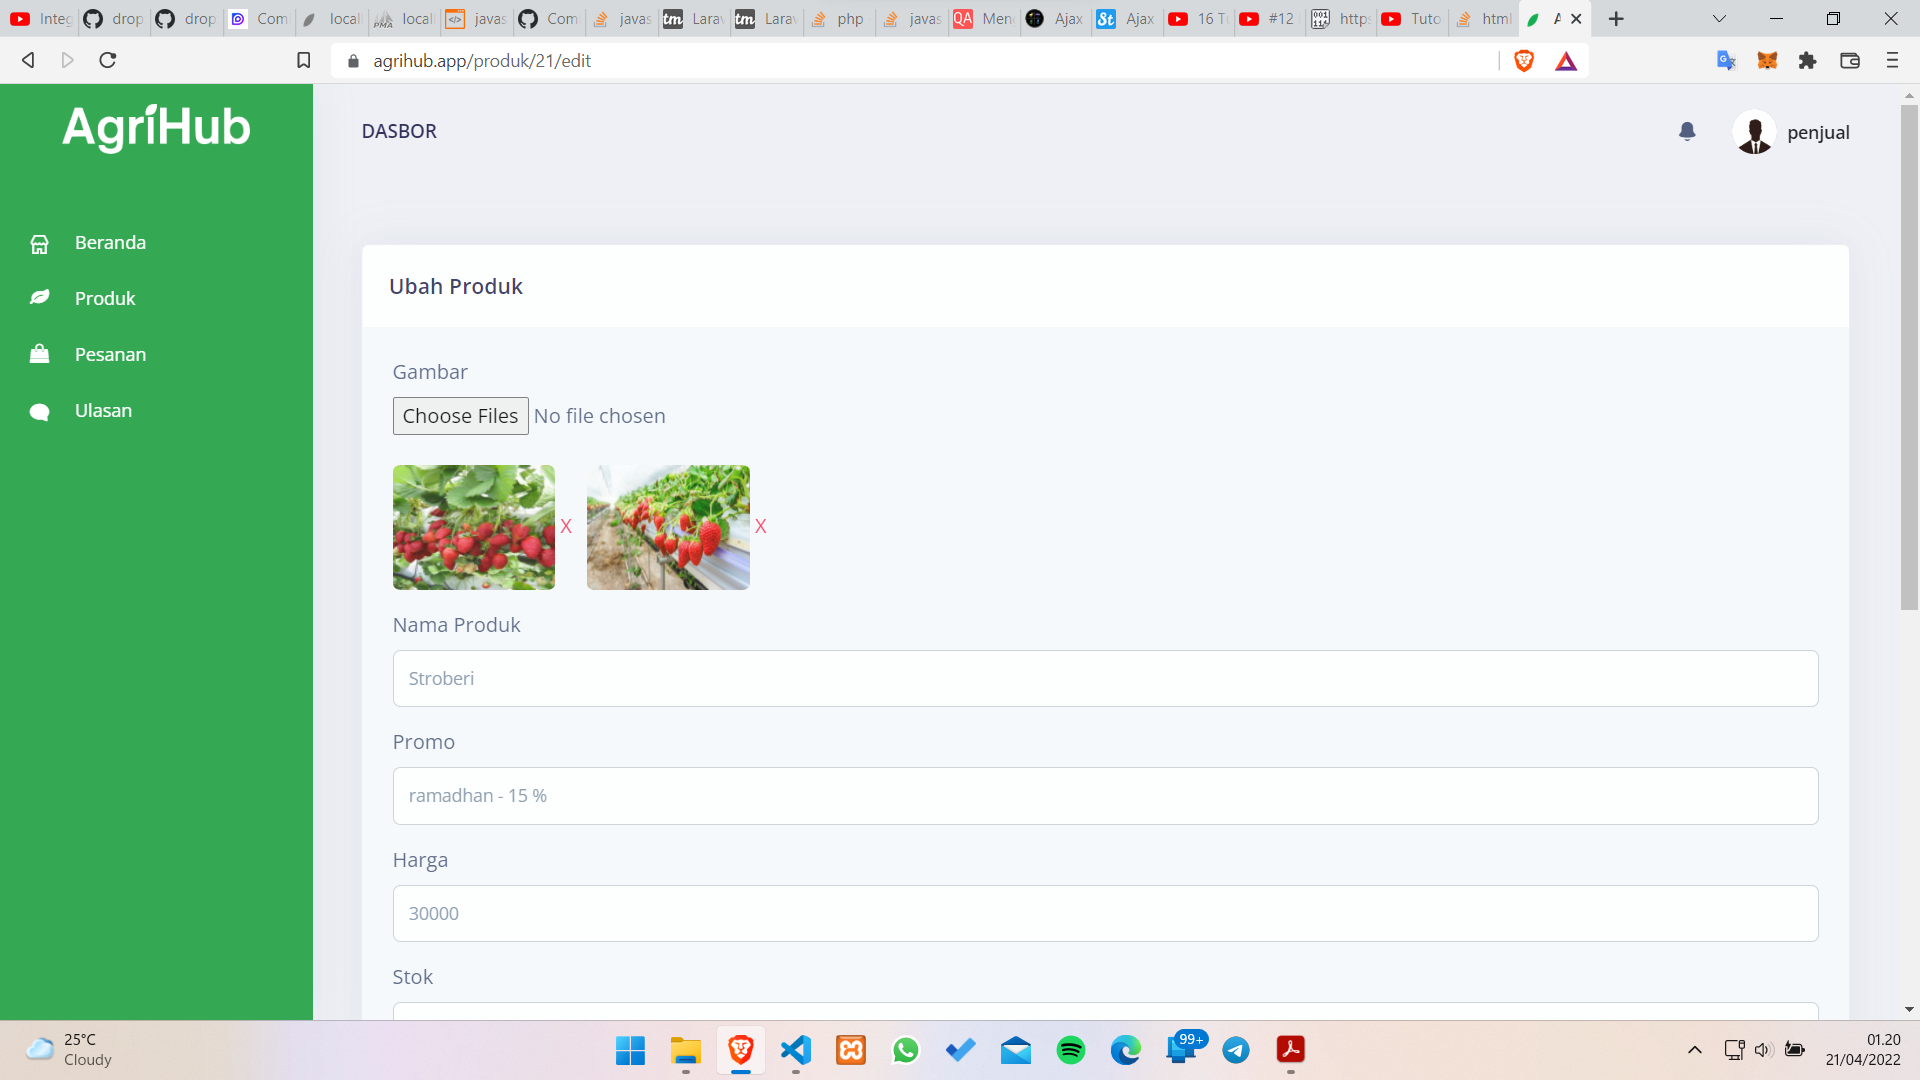
\includegraphics [width = 14.3cm, height= 9cm]{gambar/penjual/ubah_produk}}
				\caption{Halaman Ubah Produk}
				\label{ubah_produk}
			\end{figure}

			\par Apabila penjual ingin menghapus produk yang ia jual dapat menklik tombol hapus yang berwarna merah dan menekan ok untuk konfirmasi.

			\begin{figure}[H]
				\centering
				{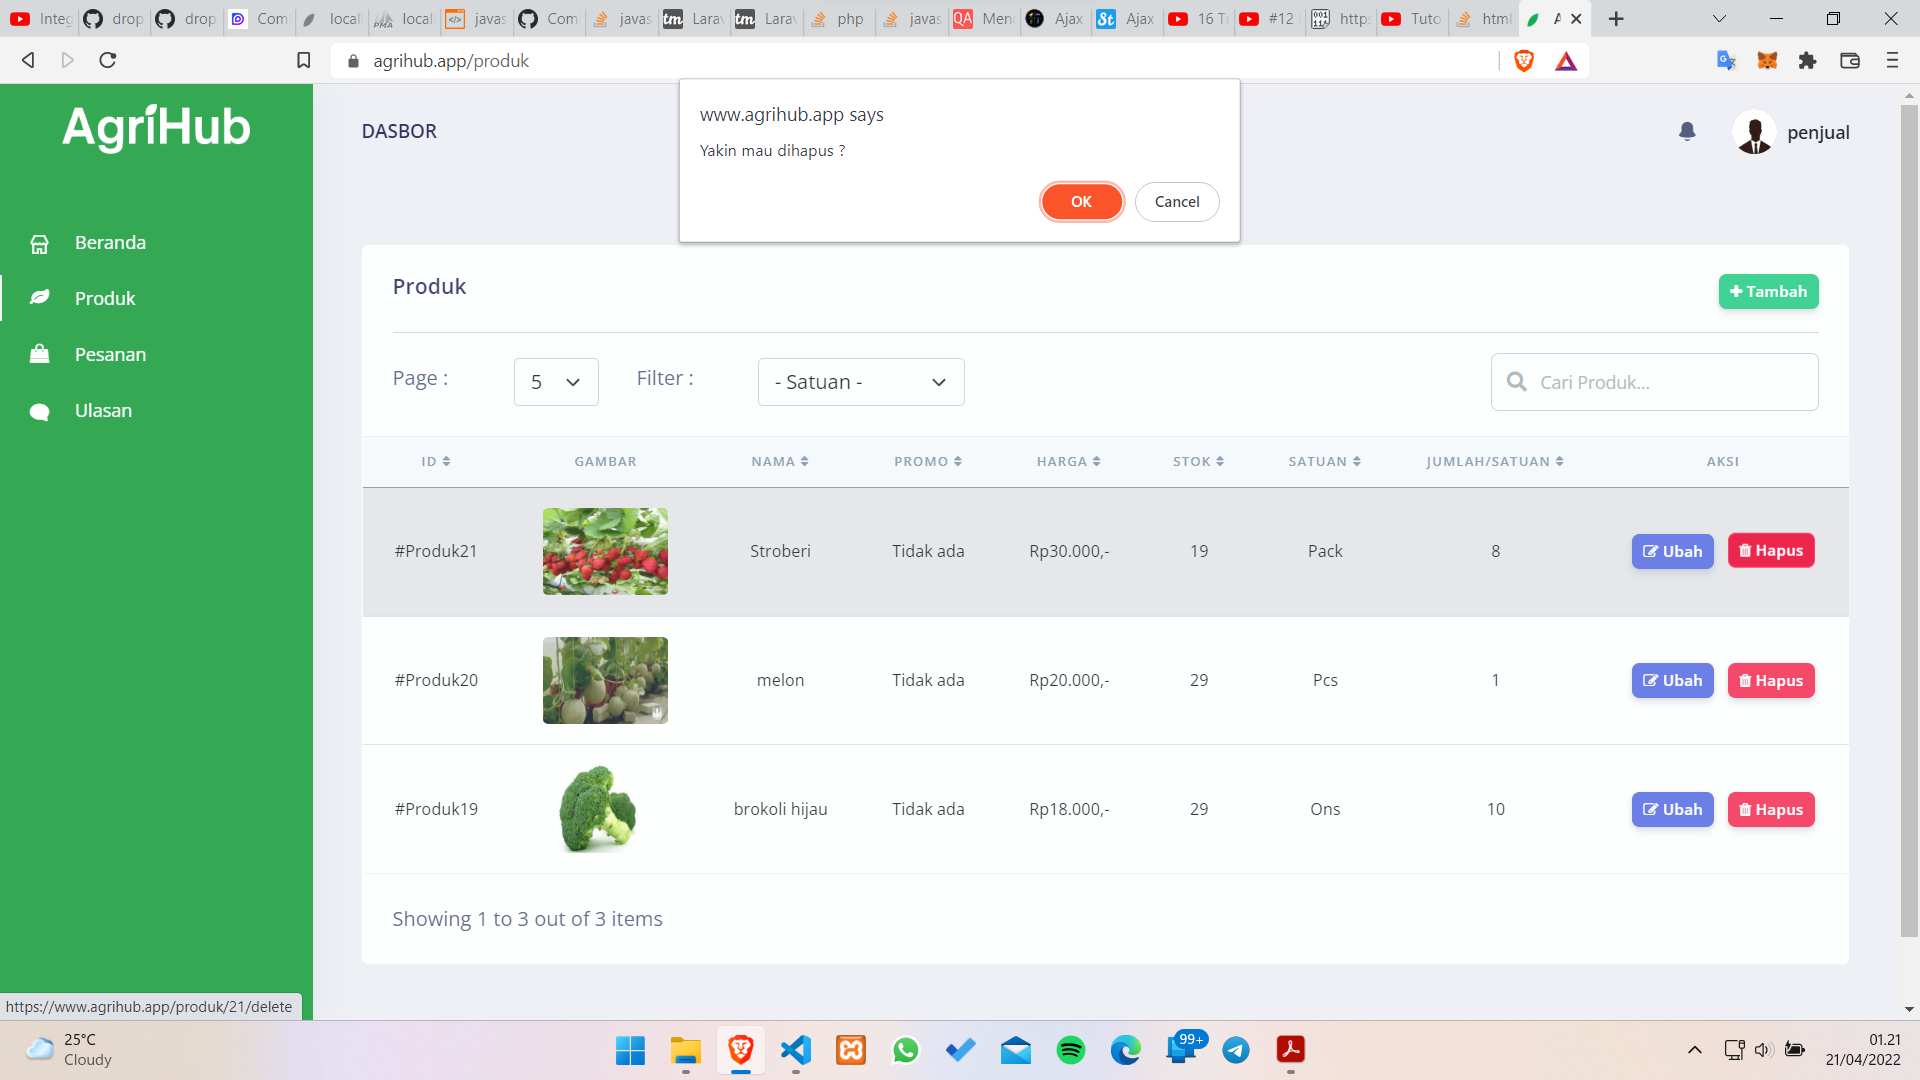
\includegraphics [width = 14.3cm, height= 9cm]{gambar/penjual/hapus_produk}}
				\caption{Halaman Hapus Produk}
				\label{hapus_produk}
			\end{figure}

			\par Selanjutnya ada halaman pesanan, halaman ini merupakan halaman yang paling penting bagi penjual karna pada halaman ini penjual mengelola semua pesanan yang masuk dari pembeli. Penjual dapat informasi mengenai pesanan seperti tanggal, jam, nama pembeli, jumlah item, ongkir dan total harganya beserta status pesanannya.

			\begin{figure}[H]
				\centering
				{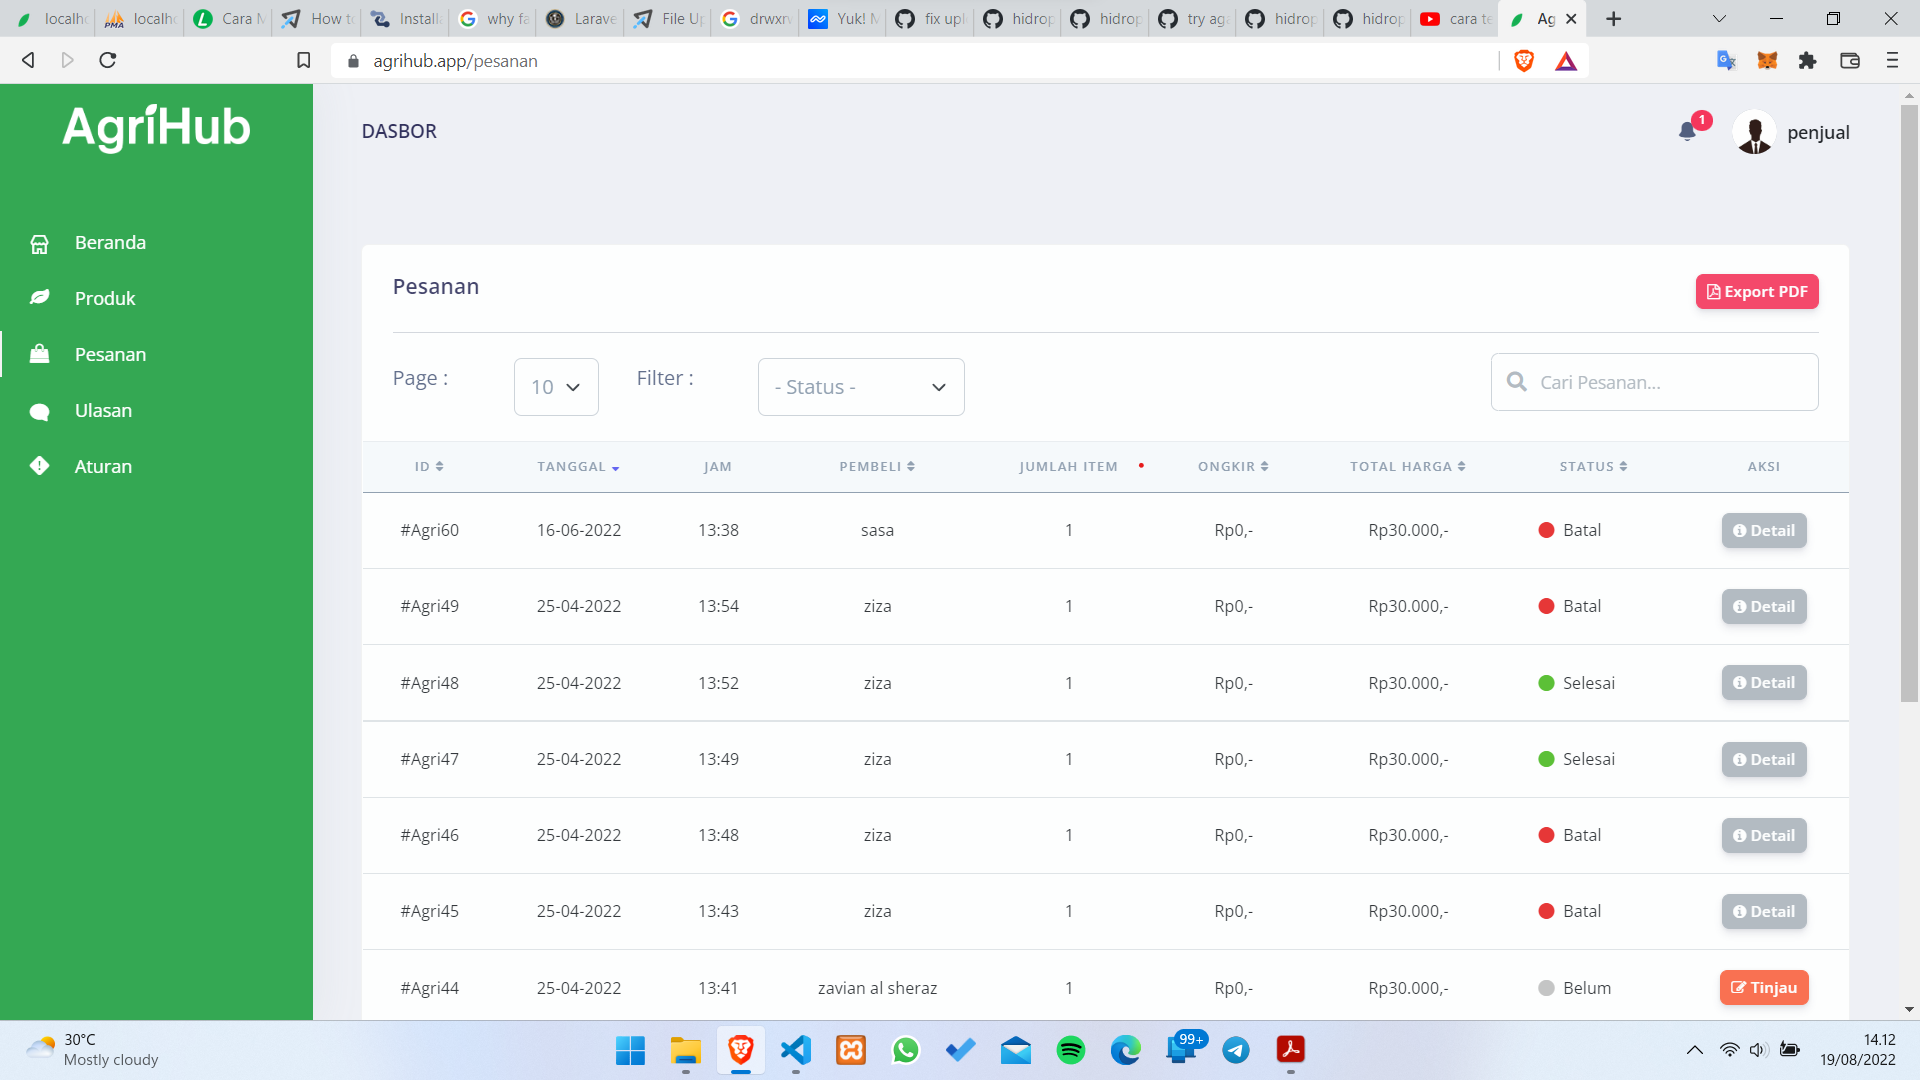
\includegraphics [width = 14.3cm, height= 9cm]{gambar/penjual/pesanan_penjual}}
				\caption{Halaman Pesanan Penjual}
				\label{pesanan_penjual}
			\end{figure}

			\par Jika penjual ingin memproses pesanan dari pembeli maka dapat menekan tombol tinjau yang berwarna orange lalu mengisi harga ongkirnya dan mengubah status pesanannya dari belum menjadi diproses. Penjual dapat menghubungi pembeli disini melalui tombol WhatApps apabila ada yang ingin ditanyakan lebih lanjut kepada pembeli. Dan penjual juga dapat menolak pesanannya dengan mengubah status menjadi batal.

			\begin{figure}[H]
				\centering
				{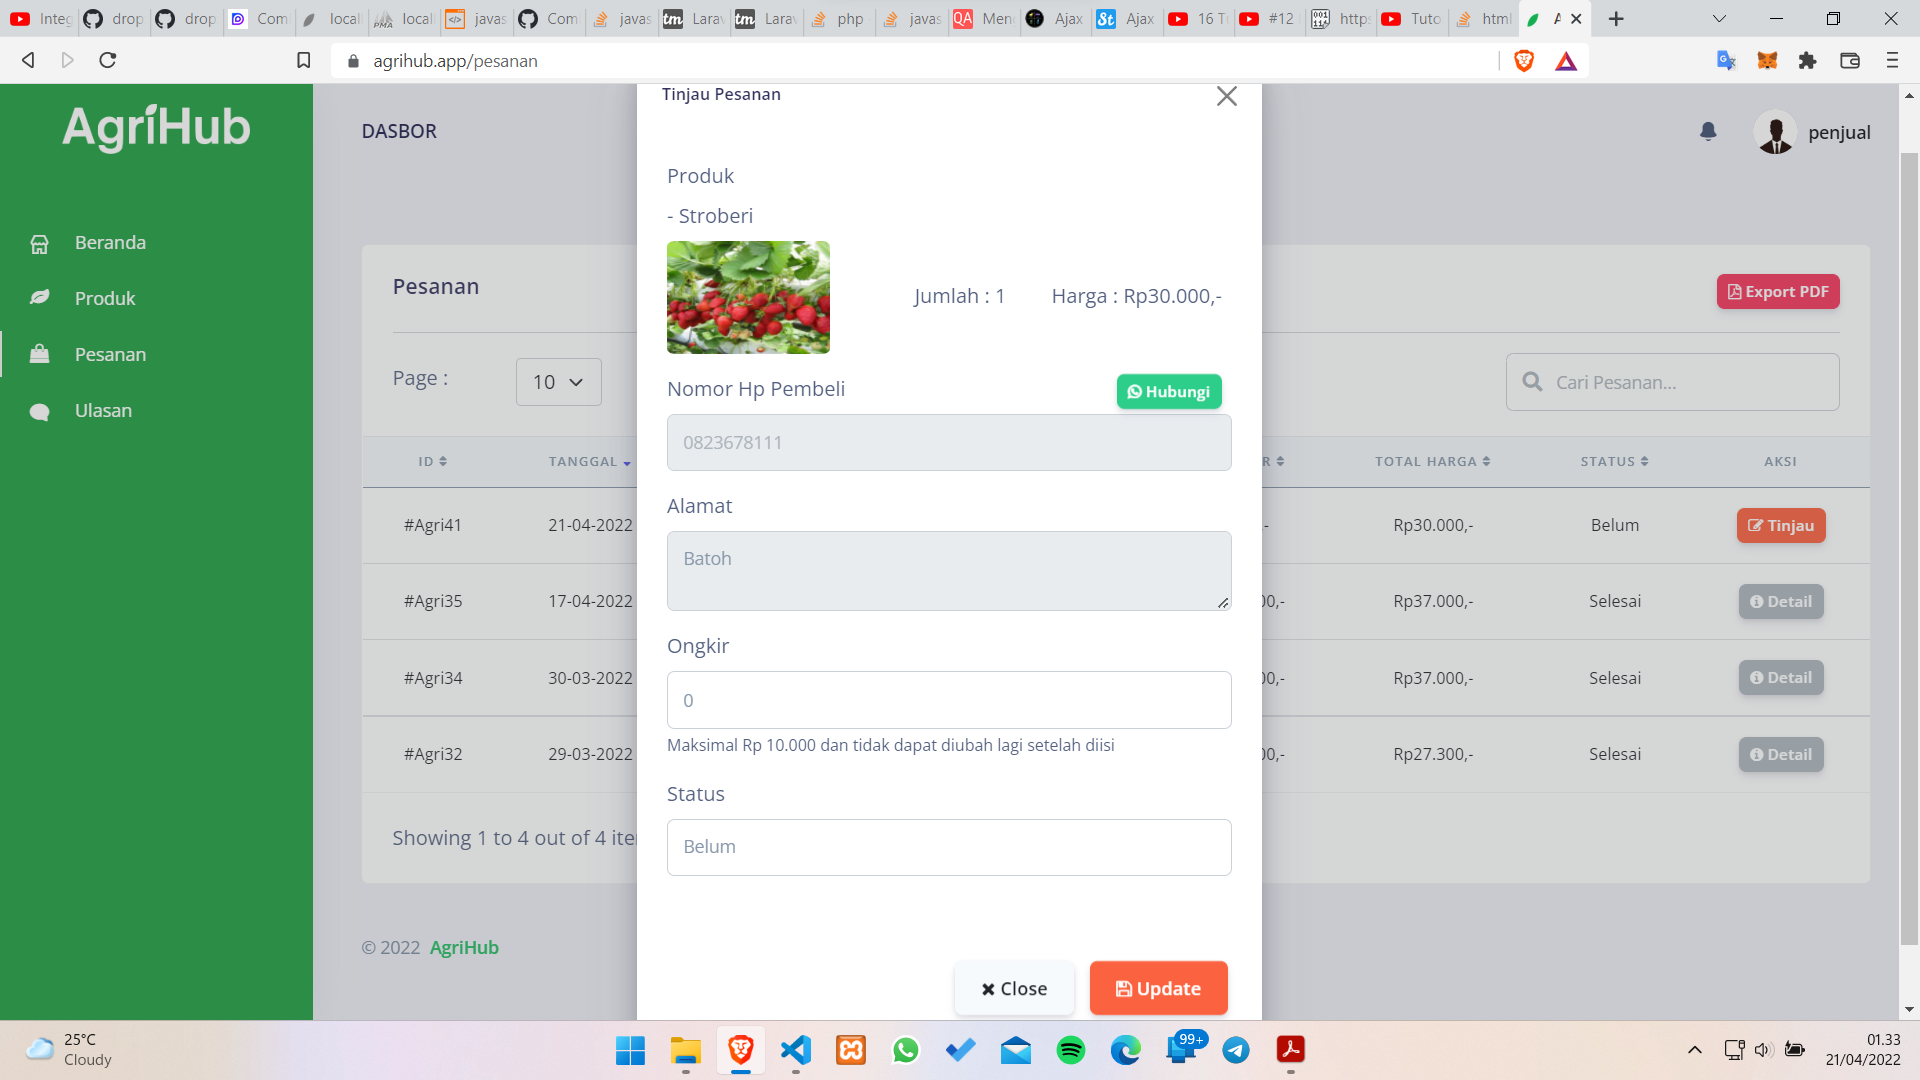
\includegraphics [width = 14.3cm, height= 9cm]{gambar/penjual/tinjau_pesanan}}
				\caption{Halaman Tinjau Pesanan}
				\label{tinjau_pesanan}
			\end{figure}

			\par Penjual juga dapat mengekspor data pesanannya dalam bentuk pdf dengan menklik tombol export pdf yang berwarna merah.

			\begin{figure}[H]
				\centering
				{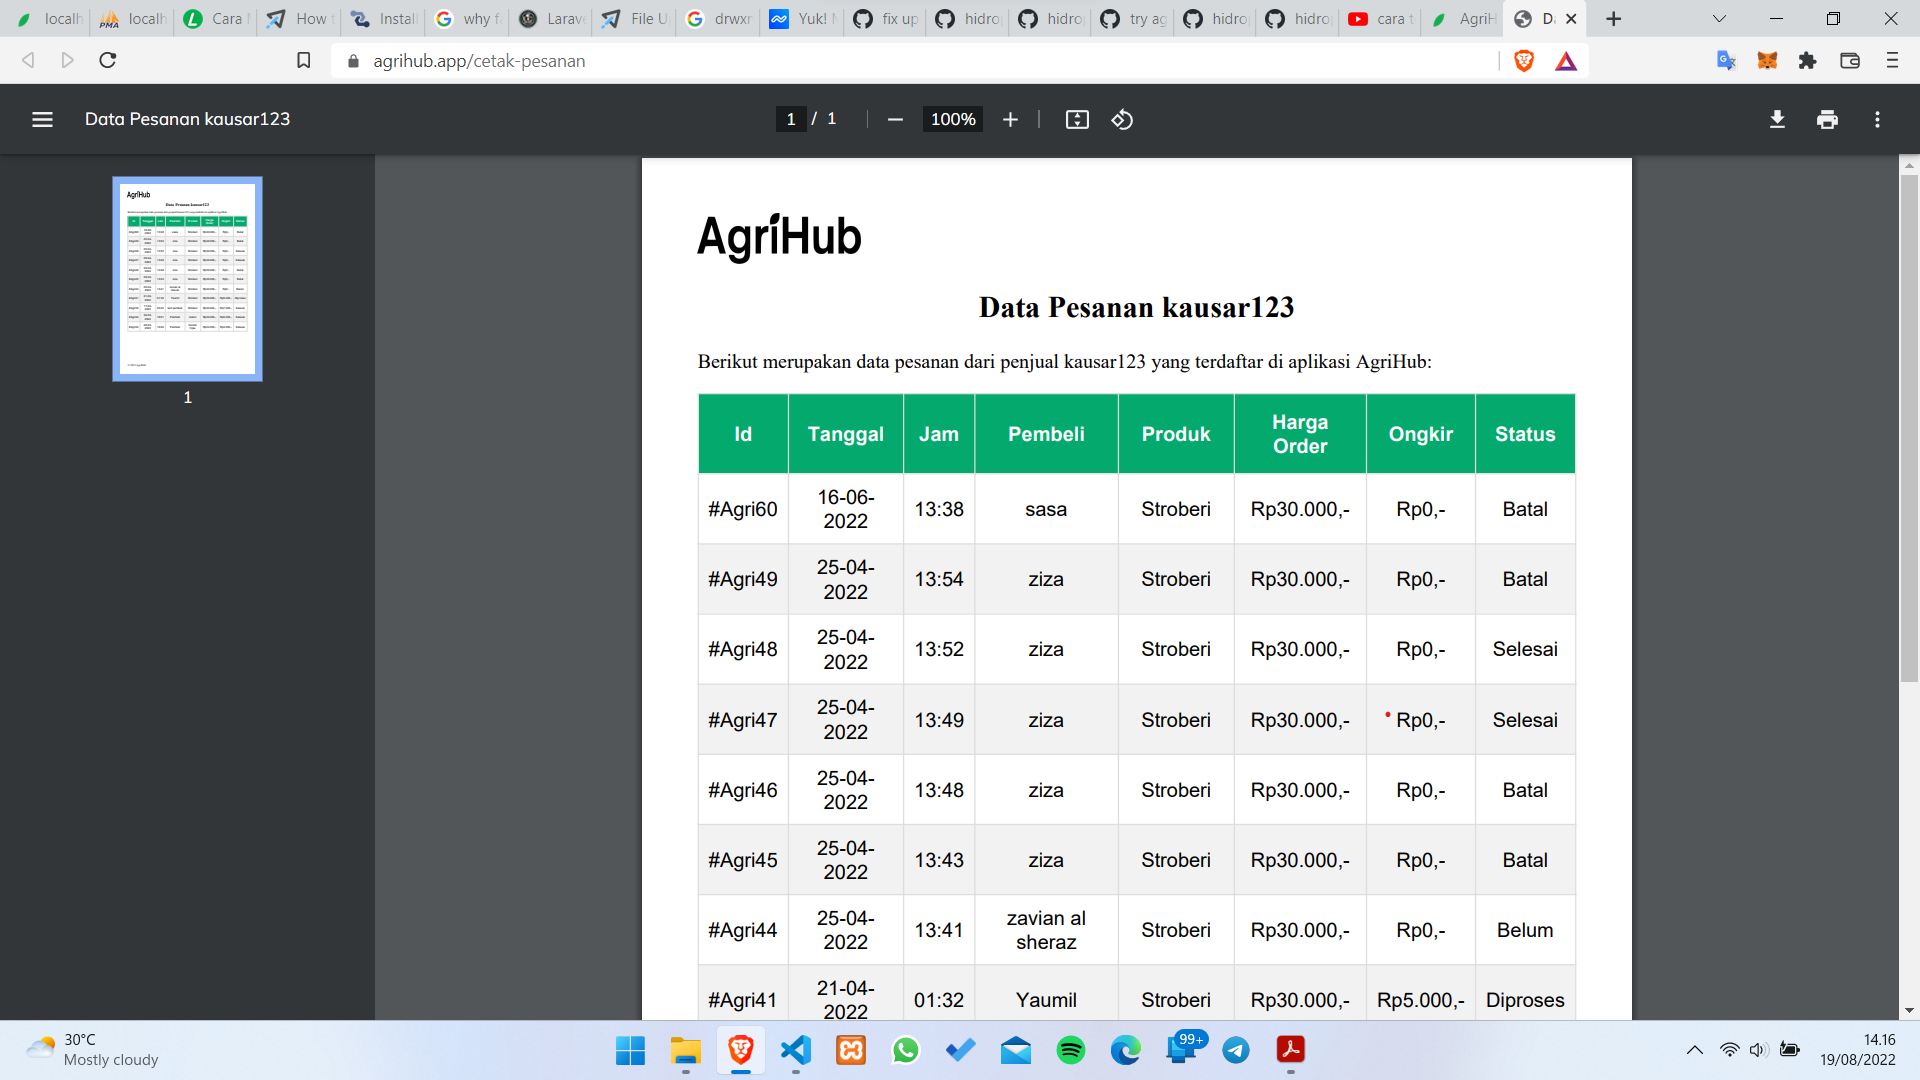
\includegraphics [width = 14.3cm, height= 9cm]{gambar/penjual/pdf_penjual}}
				\caption{Halaman Export Pesanan Penjual}
				\label{pdf_penjual}
			\end{figure}

			\par Menu terakhir ada halaman ulasan, dihalaman ini penjual dapat melihat semua ulasan yang sudah diberikan oleh pembelinya terhadap produk yang ia jual. Dari ulasan ini dapat menjadi masukan bagi penjual untuk meningkatkan lagi kualitas produk yang ia tawarkan. Serta penjual juga dapat menghapus ulasan dari pembeli jika dinilai ulasannya mengandung kata-kata yang tidak pantas.

			\begin{figure}[H]
				\centering
				{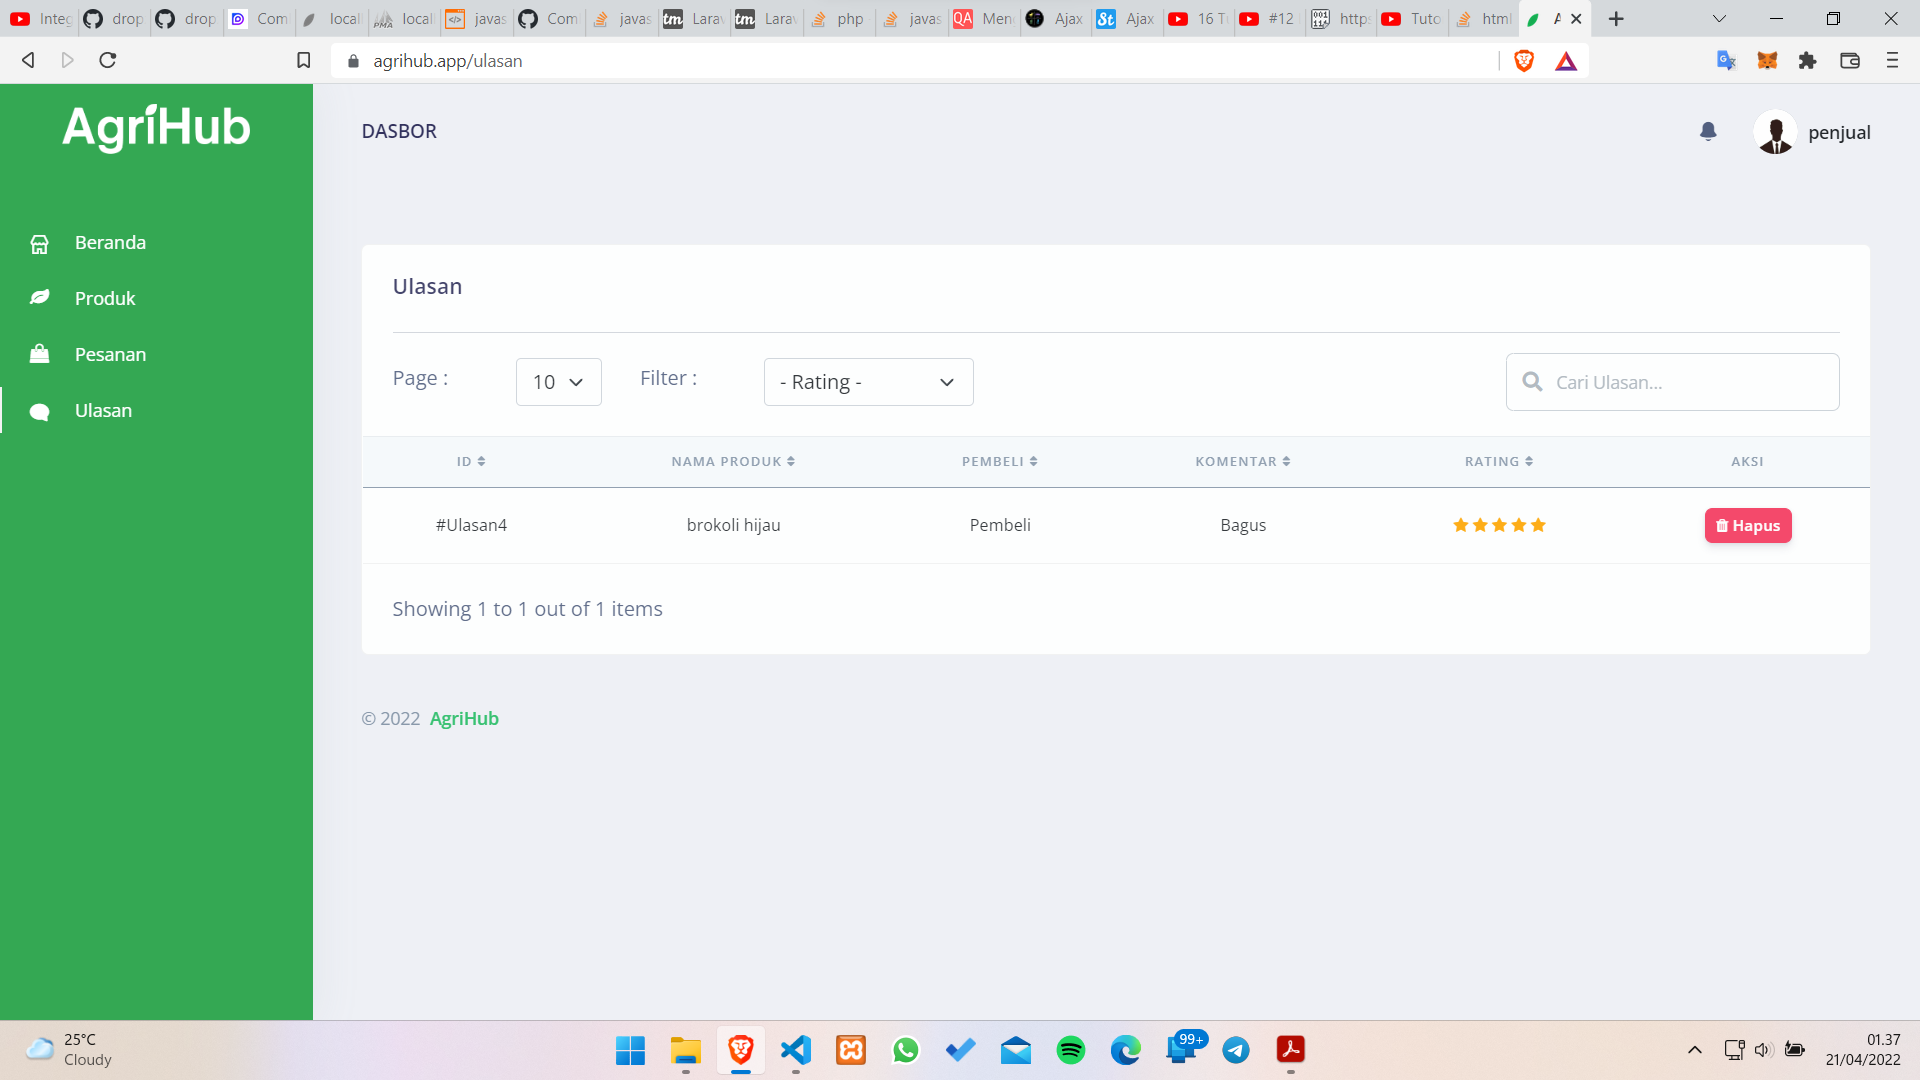
\includegraphics [width = 14.3cm, height= 9cm]{gambar/penjual/ulasan}}
				\caption{Halaman Ulasan Penjual}
				\label{ulasan}
			\end{figure}

			\par Terakhir ada halaman profil yaitu halaman dimana penjual dapat mengubah informasi mengenai dirinya sendiri seperti foto, nama, nomor hp dan alamat serta password akunnya.

			\begin{figure}[H]
				\centering
				{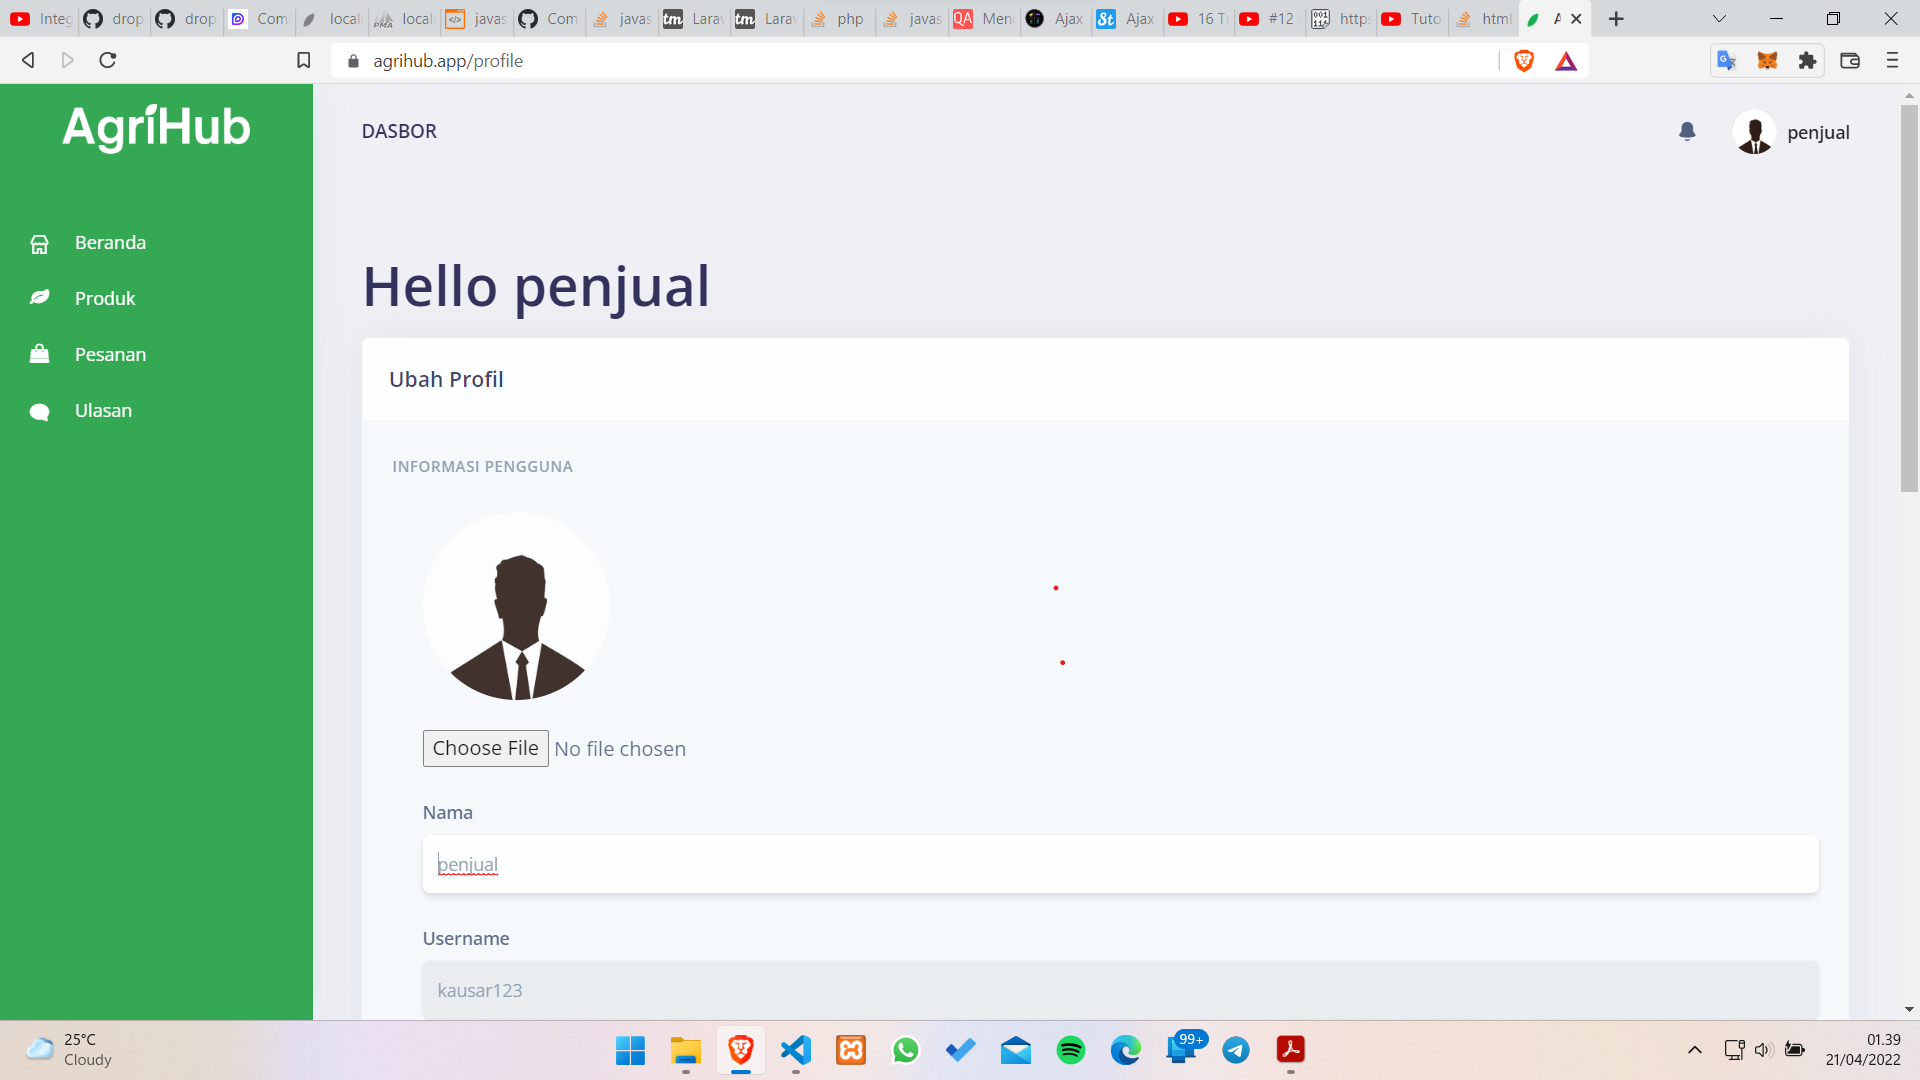
\includegraphics [width = 14.3cm, height= 9cm]{gambar/penjual/profil}}
				\caption{Halaman Profil Penjual}
				\label{profil}
			\end{figure}

		\end{enumerate}
\end{enumerate}

\subsection{\uppercase{Implementasi}}
Aplikasi jual beli tanaman hidroponik berbasis web ini dibangun
menggunakan framework Laravel dan bahasa pemrograman PHP serta database MySQL. Pada aplikasi ini juga dibuatkan API untuk menghubungkan aplikasi android dengan aplikasi web yang akan bertindak sebagai web service untuk digunakan pada aplikasi berbasis android sebagai tempat penyimpanan datanya. Aplikasi jual beli tanaman hidroponik ini juga sudah memiliki sertifikat Hak Kekayaan Intelektual (HKI) dengan nomor EC00202153104 yang dapat dilihat pada lampiran 1.

\par Aplikasi jual beli tanaman hidroponik ini dibangun menggunakan metode scrum. Metode scrum terdiri dari product backlog yang berisi daftar dari fitur yang akan diterapkan ke dalam sistem. Product backlog dibuat berdasarkan user story
yang telah dideskripsikan sesuai dengan kebutuhan sistem. user story akan menjelaskan peran setiap pengguna dalam aplikasi seperti yang terlihat pada tabel 4.1 berikut ini.

\begin{table}[H]
	\begin{center}
	\caption{User Story}
	\label{tab:jadwal}
	% \footnotesize
	\begin{tabular}{|c|l|}
	\hline
	No.&Jenis Kegiatan\\
	\hline
	1&Saya sebagai pengguna ingin melihat detail info dari produk yang dijual\\
	\hline
	2&Penulisan Proposal\\
	\hline
	3&Pengembangan Aplikasi\\
	\hline
	4&Evaluasi Sistem\\
	\hline
	5&Penulisan Laporan Akhir\\
	\hline
	\end{tabular}
	% \normalsize
	\end{center}
\end{table}

\par Setelah mengumpulkan user story, selanjutnya adalah membuat product
baklog dari user story tersebut yang implementasinya akan dibagi dalam beberapa
bagian sprint atau iterasi. Pada penelitian ini, terdapat 4 kali iterasi sprint. Berikut
merupakan pembagian product backlog ke dalam beberapa iterasi :

\begin{enumerate}
	\item Sprint Pertama
	\par Pada sprint pertama, fitur yang difokuskan pada sprint ini merupakan fitur-fitur
	yang dianggap mempunyai prioritas yang lebih tinggi dibandingkan fitur yang lain
	seperti: fitur daftar akun, masuk akun, lihat produk, tambahkan ke keranjang, dan
	proses membeli produk. Adapun untuk daftar product backlog pada sprint yang
	pertama dapat dilihat pada tabel 4.2 berikut ini.

	\begin{table}[H]
		\begin{center}
		\caption{Product Backlog sprint pertama}
		\label{tab:jadwal}
		% \footnotesize
		\begin{tabular}{|c|l|}
		\hline
		No.&Jenis Kegiatan\\
		\hline
		1&Saya sebagai pengguna ingin melihat detail info dari produk yang dijual\\
		\hline
		2&Penulisan Proposal\\
		\hline
		3&Pengembangan Aplikasi\\
		\hline
		4&Evaluasi Sistem\\
		\hline
		5&Penulisan Laporan Akhir\\
		\hline
		\end{tabular}
		% \normalsize
		\end{center}
	\end{table}

	\par Kendala yang dihadapi pada sprint pertama yaitu belum adanya server resmi yang
	disediakan untuk aplikasi jual tanaman hidroponik berbasis web. Sehingga untuk
	beberapa saat, aplikasi jual tanaman hidroponik berbasis web ini menggunakan
	hosting milik pribadi. Hal ini harus dilakukan karena untuk mengimplementasikan
	REST API pada aplikasi berbasis android, maka harus terlebih dahulu melakukan
	deployment aplikasi berbasis web ke server atau hosting.
	Ketika API pada aplikasi berbasis web sudah bisa diakses, selanjutnya untuk
	menghubungkan antara aplikasi berbasis android dengan aplikasi berbasis web
	digunakan REST API dengan metode GET, DELETE, dan POST. Bentuk datanya
	sendiri adalah dalam format json. Berikut ini merupakan gambaran bentuk data
	produk yang digunakan.

	\item Sprint Kedua
	\par Pada sprint kedua ini, dilakukan penyempurnaan dari fitur-fitur yang telah dibuat
	pada sprint pertama seperti penambahan frontend, penambahan beberapa tombol
	yang terhubung dengan API dan halaman (screen) baru. Tingkat prioritas pada
	tahap sprint kedua didominasi oleh tingkatan prioritas sedang. Daftar product
	backlog pada sprint kedua dapat dilihat pada tabel 4.3 berikut ini.

	\begin{table}[H]
		\begin{center}
		\caption{Product Backlog sprint pertama}
		\label{tab:jadwal}
		% \footnotesize
		\begin{tabular}{|c|l|}
		\hline
		No.&Jenis Kegiatan\\
		\hline
		1&Saya sebagai pengguna ingin melihat detail info dari produk yang dijual\\
		\hline
		2&Penulisan Proposal\\
		\hline
		3&Pengembangan Aplikasi\\
		\hline
		4&Evaluasi Sistem\\
		\hline
		5&Penulisan Laporan Akhir\\
		\hline
		\end{tabular}
		% \normalsize
		\end{center}
	\end{table}
\end{enumerate}

\section{\uppercase{Pengujian}}
Pengujian sistem dilakukan dengan melibatkan 2 tipe user yaitu admin dan penjual, untuk jumlah usernya 5 orang admin dan 5 orang penjual, dan untuk adminnya diuji kepada mitra penjual awal yang dianggap sebagai admin nantinya sedangkan untuk penjualnya diuji kepada mitra penjual yang sudah ada dan calon penjual. Pada penelitian ini akan dilakukan 2 pengujian yaitu pengujian fungsionalitas dan pengujian \textit{usability}.

\begin{enumerate}
	\item Pengujian Fungsionalitas Menggunakan Black Box
	\par Pengujian fungsionalitas pada aplikasi jual beli tanaman hidroponik berbasis web dilakukan menggunakan metode black box. Pengujian fungsionalitas pada penelitian ini dilakukan secara manual dengan penguji akan bertindak sebagai pengguna aplikasi. Metode black box hanya akan berfokus pada apa yang menjadi nilai masukkan dan keluaran dari aplikasi sehingga tidak perlu untuk memahami struktur code di dalam aplikasi. Metode black box ini dapat digunakan untuk mengetahui apakah aplikasi jual beli tanaman hidroponik berbasis android dapat berfungsi dengan baik atau tidak.

	\begin{table}[H]
		\begin{center}
		\caption{Tabel Black Box}
		\label{tab:jadwal}
		% \footnotesize
		\begin{tabular}{|c|c|c|c|c|}
		\hline
		No.&Nama Pengujian&Skenario&tampilan&Kesimpulan\\
		\hline
		\multirow{2}{*}{1}&\multirow{2}{*}{Melihat produk yang dijual di dalam sistem}&\multirow{2}{*}{membuka aplikasi dengan internet yang hidup}&\multirow{2}{*}{diarahkan ke beranda}&\multirow{2}{*}{sesuai}\\
		\hline
		\multirow{2}{*}{1}&\multirow{2}{*}{Melihat produk yang dijual di dalam sistem}&\multirow{2}{*}{membuka aplikasi dengan internet yang hidup}&\multirow{2}{*}{diarahkan ke beranda}&\multirow{2}{*}{sesuai}\\
		\hline
		\multirow{2}{*}{1}&\multirow{2}{*}{Melihat produk yang dijual di dalam sistem}&\multirow{2}{*}{membuka aplikasi dengan internet yang hidup}&\multirow{2}{*}{diarahkan ke beranda}&\multirow{2}{*}{sesuai}\\
		\hline
		\multirow{2}{*}{1}&\multirow{2}{*}{Melihat produk yang dijual di dalam sistem}&\multirow{2}{*}{membuka aplikasi dengan internet yang hidup}&\multirow{2}{*}{diarahkan ke beranda}&\multirow{2}{*}{sesuai}\\
		\hline
		\multirow{2}{*}{1}&\multirow{2}{*}{Melihat produk yang dijual di dalam sistem}&\multirow{2}{*}{membuka aplikasi dengan internet yang hidup}&\multirow{2}{*}{diarahkan ke beranda}&\multirow{2}{*}{sesuai}\\
		\hline
		\multirow{2}{*}{1}&\multirow{2}{*}{Melihat produk yang dijual di dalam sistem}&\multirow{2}{*}{membuka aplikasi dengan internet yang hidup}&\multirow{2}{*}{diarahkan ke beranda}&\multirow{2}{*}{sesuai}\\
		\hline
		\multirow{2}{*}{1}&\multirow{2}{*}{Melihat produk yang dijual di dalam sistem}&\multirow{2}{*}{membuka aplikasi dengan internet yang hidup}&\multirow{2}{*}{diarahkan ke beranda}&\multirow{2}{*}{sesuai}\\
		\hline
		\multirow{2}{*}{1}&\multirow{2}{*}{Melihat produk yang dijual di dalam sistem}&\multirow{2}{*}{membuka aplikasi dengan internet yang hidup}&\multirow{2}{*}{diarahkan ke beranda}&\multirow{2}{*}{sesuai}\\
		\hline
		\multirow{2}{*}{1}&\multirow{2}{*}{Melihat produk yang dijual di dalam sistem}&\multirow{2}{*}{membuka aplikasi dengan internet yang hidup}&\multirow{2}{*}{diarahkan ke beranda}&\multirow{2}{*}{sesuai}\\
		\hline
		\multirow{2}{*}{1}&\multirow{2}{*}{Melihat produk yang dijual di dalam sistem}&\multirow{2}{*}{membuka aplikasi dengan internet yang hidup}&\multirow{2}{*}{diarahkan ke beranda}&\multirow{2}{*}{sesuai}\\
		\hline
		\end{tabular}
		% \normalsize
		\end{center}
	\end{table}

	\par Berdasarkan data dari tabel 4.7, maka dapat diketahui bahwa aplikasi jual beli tanaman hidroponik berbasis android dapat berjalan dengan baik. Hal ini dapat dilihat
	dari hasil pengujian black box yang telah dilakukan ada setiap fitur di dalam aplikasi memiliki hasil "Sesuai".

	\item Pengujian \textit{Usability} Menggunakan Metode UMUX
	\par Pengujian usability dilakukan dengan tujuan untuk melihat apakah aplikasi dapat secara efisien digunakan oleh pengguna. Pengujian usability secara keseluruhan akan berfokus pada desain dan bagaimana interaksi antara pengguna dan aplikasi. Jika dengan penggunaan aplikasi dapat menjadikan pengguna lebih mudah dalam mencapai tujuannya, maka aplikasi tersebut akan dianggap mempunyai usability yang baik. Pada penelitian ini, pengujian usability akan dilakukan menggunakan metode UMUX. Pengujian UMUX dilakukan dengan memberikan kuesioner kepada 20 responden. Responden dapat menjawab pertanyaan yang ada pada kuesioner. Hasil pengujian akan ditampilkan pada tabel berikut ini.

	\begin{table}[H]
		\begin{center}
		\caption{Tabel UMUX}
		\label{tab:jadwal}
		% \footnotesize
		\begin{tabular}{|c|c|c|c|c|c|}
		\hline
		\multirow{2}{*}{Responden}&\multicolumn{4}{c|}{Kode Pertanyaan}&\multirow{2}{*}{Skor}\\
		\cline{2-5}
		&P1&P2&P3&P4&\\
		\hline
		1&6&1&7&1&95\\
		\hline
		2&6&1&7&1&95\\
		\hline
		3&6&1&7&1&95\\
		\hline
		4&6&1&7&1&95\\
		\hline
		5&6&1&7&1&95\\
		\hline
		6&6&1&7&1&95\\
		\hline
		7&6&1&7&1&95\\
		\hline
		8&6&1&7&1&95\\
		\hline
		9&6&1&7&1&95\\
		\hline
		10&6&1&7&1&95\\
		\hline
		\multicolumn{5}{|c|}{Rata-rata}&89\\
		\hline
		\end{tabular}
		% \normalsize
		\end{center}
	\end{table}

	\par Berdasarkan hasil pengujian pada tabel di atas didapatkan skor rata-rata sebesar 89,58. Skor tersebut menunjukkan bahwa aplikasi ini memiliki nilai dapat diterima.
\end{enumerate}

%-----------------------------------------------------------------------------%

% Baris ini digunakan untuk membantu dalam melakukan sitasi
% Karena diapit dengan comment, maka baris ini akan diabaikan
% oleh compiler LaTeX.
\begin{comment}
\bibliography{daftar-pustaka}
\end{comment}